\documentclass[11pt,twoside,openright]{moddalthesis}

\usepackage{hyperref}

\usepackage[spanish,english]{babel}
%\usepackage[spanish]{babel}
%\usepackage[latin1]{inputenc}
\usepackage[utf8]{inputenc}
\usepackage{CJKutf8}


%-------------------------------------
\usepackage{chronology}
\usepackage{epigraph}

\usepackage{graphicx}
\usepackage{color}

\usepackage[symbols,nogroupskip,nonumberlist,sort=use]{glossaries-extra}


%\usepackage[backend=biber,style=alphabetic,citestyle=authoryear]{biblatex}

%\usepackage{natbib}    % Change bibstyle.

\usepackage{amsmath}
\usepackage{amsfonts}
\usepackage{amssymb}
%\usepackage{subfig}
\usepackage{subfigure} 

\usepackage{amsthm}
\theoremstyle{definition}
\newtheorem{definition}{Definition}[section]


\usepackage{booktabs}
\usepackage{siunitx}
\sisetup{math-micro=\text{µ},text-micro=µ}

%--------
\usepackage[many]{tcolorbox}
\usepackage{marginnote}
\usepackage{kantlipsum}
\tcbuselibrary{skins,breakable}
\newtcolorbox{story}[1][]{
    width=\textwidth,
    colback=magenta!20,
    colframe=red!75!black,
    colbacktitle=blue!85!black,
    fonttitle=\bfseries,
    left=0ex,
    right=0ex,
    top=0pt,
    arc=0pt,
    outer arc=0pt,
    leftrule=0pt,
    rightrule=0pt,
    toprule=0pt,
    bottomrule=0pt,
    breakable,
    enhanced jigsaw,
    title= #1}
\hypersetup{hidelinks=true}    
\usepackage{eso-pic}
\newcommand\AlCentroPagina[1]{% 
\AddToShipoutPicture*{\AtPageCenter{% 
\makebox(0,0){\hspace*{3cm}\includegraphics% 
[width=0.9\paperwidth]{#1}}}}}    
%-------

\newcommand{\blankpage}{
\newpage
\thispagestyle{empty}
\mbox{}
\newpage
}

\makenoidxglossaries

\glsxtrnewsymbol[description={Signal Segment Size}]{w}{\ensuremath{w}}
\glsxtrnewsymbol[description={Sample points}]{N}{\ensuremath{N}}
\glsxtrnewsymbol[description={Number of available channels}]{C}{\ensuremath{C}}
\glsxtrnewsymbol[description={Signal Span}]{lambda}{\ensuremath{\lambda}}
\glsxtrnewsymbol[description={Sampling Frequency}]{Fs}{\ensuremath{F_s}}
\glsxtrnewsymbol[description={Pixels in unit scale}]{Deltas}{\ensuremath{\Delta_s}}
\glsxtrnewsymbol[description={Peak-to-peak Amplitude}]{DeltamuV}{\ensuremath{\Delta \mu V}}
\glsxtrnewsymbol[description={Signal Amplitude Scale Factor}]{gamma}{\ensuremath{\gamma}}
\glsxtrnewsymbol[description={Time Scale Factor}]{gammat}{\ensuremath{\gamma_t}}
\glsxtrnewsymbol[description={Image Height}]{Hy}{\ensuremath{H_y}}
\glsxtrnewsymbol[description={Image Width}]{Wx}{\ensuremath{W_x}}
\glsxtrnewsymbol[description={Horizontal Patch Scale}]{St}{\ensuremath{S_t}}
\glsxtrnewsymbol[description={Vertical Patch Scale}]{Sv}{\ensuremath{S_v}}
\glsxtrnewsymbol[description={Patch Height}]{Sy}{\ensuremath{\mathbf{S}_y}}
\glsxtrnewsymbol[description={Patch Width}]{Sx}{\ensuremath{\mathbf{S}_x}}
\glsxtrnewsymbol[description={Keypoint}]{kp}{\ensuremath{\mathbf{kp}}}
\glsxtrnewsymbol[description={Pixel}]{P}{\ensuremath{\mathbf{p}}}
\glsxtrnewsymbol[description={Descriptor}]{d}{\ensuremath{\mathbf{d}}}
\glsxtrnewsymbol[description={Keypoint Density}]{kpd}{\ensuremath{\mathbf{kp_d}}}
\glsxtrnewsymbol[description={Intensification Sequences Repetitions}]{ka}{\ensuremath{k_a}}
\glsxtrnewsymbol[description={Best Performing Channel}]{bpc}{\ensuremath{bpc}}


%$\gls{N}$, $\gls{\lambda}$, $\gls{F_s}$, $\gls{\Delta_s}$, $\gls{\Delta \mu V}$.

%\includeonly{FrontBackmatter/Contents,Chapters/Chapter03,Chapters/Chapter04,Chapters/Chapter05,Chapters/Chapter06,Chapters/Chapter0A,FrontBackmatter/Bibliography}

%\includeonly{Chapters/Chapter01,Chapters/Chapter02}

%-------------------------------------

%\addbibresource{Bibliography.bib}    % Use with biblatex

\begin{document}

\AlCentroPagina{images/itbalogoshaded}

\title{\textbf{Histogram of Gradient Orientations of EEG Signal Plots for Brain Computer Interfaces}}
\author{Rodrigo Ramele}
\dept{Doctorado}
\faculty{Escuela de Ingeniería en Informática}
\university{Instituto Tecnológico de Buenos Aires}
\address{Buenos Aires, Argentina}

\submitdate{30 de Noviembre, 2018}
\defencedate{Mes Día, 2018}
\copyrightyear{2018}
\convocation{Mes}{Año}

%\phd
\degree{Doctor en Ingeniería Informatica}
\degreeinitial{Doctor en Ingeniería Informatica}

\supervisor{Dr. Juan Miguel Santos}
\supervisor{Dra. Ana Julia Villar}

\firstreader{Dra. Jurado}
\secondreader{Dr. Jurado}
\thirdreader{Dr. Jurado}


%%% ZONA PARA LA PRIMERA PAGINA EN SP
%\title{\textbf{Titulo en Espanol}}
%\dept{Ingenier\'ia en Inform\'atica}
%\faculty{Ingenier\'ia}
%\university{Instituto Tecnol\'ogico de Buenos Aires}
%\address{Buenos Aires, Argentina}
%%
%\submitdate{Month Day, Year}
%\defencedate{Month Day, Year}
%\copyrightyear{Year}
%\convocation{Month}{Year}
% FINNNNN


\dedicate{\begin{CJK}{UTF8}{min}希望がある所に道もあります\end{CJK}}

%\nodedicationpage
%\notableofcontents
\nolistoftables
\nolistoffigures

%{
%\typeout{:?000000000} % Don't bother with over/under-full boxes
\beforepreface
%\typeout{:?111111111} % Process All Errors from Here on
%}

%\begin{abstract}
%Brain Computer Interface (BCI) or Brain Machine Interfaces (BMI), has proved the feasibility of a distinct non-biological communication channel to transmit information from the Central Nervous System (CNS) to a computer device.  Promising success has been achieved with invasive BCI, though biocompatibilities issues and the complexity and risks of surgical procedures are the main drive to enhance current non-invasive technologies.
%
%Electroencephalography (EEG) is the most widespread method to gather information from the CNS in a non-invasive way.  Clinical EEG has traditionally focused on temporal waveforms, but signal analysis methods which follow this path has been overshadow in BCI research. 
%
%This thesis propose a method and framework to analyze the waveform, the shape of the EEG signal, using the histogram of gradient orientations, a fruitful technique from Computer Vision which is used to depict image local characteristics. This method generates a feature, a 128-dimension descriptor, that  is used to to analyze the underlying cognitive phenomena. Inspiration comes from what traditionally electroencephalographers have been doing for almost a century: visually inspecting raw EEG signal plots. 
%
%The validity of the method is verified by identifying Visual Occipital Alpha Waves and Motor Imagery Rolandinc Mu rhythms. It is also applied on P300 ERP detection and used to implement a P300-Based Visual Speller application. Experimental protocols to produce these cognitive patterns were designed and own datasets produced and published using both commercial-grade and research-grade EEG devices.  Obtained results on public and own datasets are outlined, and comparisons performed against similar procedures.
%
%The benefits of the approach presented here are twofold, (1) it has a universal applicability because the same basic methodology can be applied to detect different patterns in EEG signals with applications to BCI and (2) it has the potential to foster close collaboration with physicians and electroencephalograph technicians because this direction of work follows the established procedure of the clinical EEG community of analyzing waveforms by their shapes.
%\end{abstract}


\begin{abstract}

Brain Computer Interface (BCI) or Brain Machine Interfaces (BMI), has proved the feasibility of a distinct non-biological communication channel to transmit information from the Central Nervous System (CNS) to a computer device.  Promising success has been achieved with invasive BCI, though biocompatibilities issues and the complexity and risks of surgical procedures are the main drive to enhance current non-invasive technologies.  

Electroencephalography (EEG) is the most widespread method to gather information from the CNS in a non-invasive way.  Clinical EEG has traditionally focused on temporal waveforms, but signal analysis methods which follow this path has been overshadow in BCI research. 

This thesis propose a method and framework to analyze the waveform, the shape of the EEG signal, using the histogram of gradient orientations, a fruitful technique from Computer Vision which is used to characterize image local features. Inspiration comes from what traditionally electroencephalographers have been doing for almost a century: visually inspecting raw EEG signal plots. 

This technique can be outlined in five steps, (1) signal preprocessing, (2) signal segmentation, (3) transformation on a channel by channel basis of each signal segment into a binary image of a signal plot, (4) assignment of keypoint location on a position over the newly created image depending on the physiological phenomena under study and finally (5) the calculation of the histogram of gradient orientations using finite differences from the image around this keypoint. This method generates a feature, a normalized 128-dimension descriptor. This feature is used to compare the signal segments that were used to generate them, hence to analyze the underlying cognitive phenomena. 

The validity of the method is verified by studying three cognitive patterns.  First, Visual Occipital Alpha Waves are analyzed.  An experimental protocol is designed and a dataset is produced using a commercial-grade EEG device.  Additionally, the ability of the method to capture oscillatory processes is verified by analyzing a public dataset. Moreover, this methodology is extended to study a related oscillatory process: Motor Imagery Rolandic Mu rhythms.  The performance of the method to discriminate right vs left motor imagery against a public dataset of healthy subjects, is verified.  Results are informed and reported. 

Finally, the method is modified to capture transient events, particularly the P300 Event Related Potential (ERP).  A description on how to extract the ERP from the EEG segment is offered, and a detailed depiction of how to implement a P300-Based BCI Speller application is outlined.  Its performance is verified by processing a public dataset of Amiotrophic Lateral Sclerosis (ALS) patients and contrasted against an own dataset produced in-house replicating the same experimental conditions.  Results are compared against other methods referenced in the bibliography

The benefits of the approach presented here are twofold, (1) it has a universal applicability because the same basic methodology can be applied to detect different patterns in EEG signals with applications to BCI and (2) it has the potential to foster close collaboration with physicians and electroencephalograph technicians because this direction of work follows the established procedure of the clinical EEG community of analyzing waveforms by their shapes.


%In recent years, the idea of a direct interface between the human brain and an artificial system, called Brain Computer Interface (BCI) or Brain Machine Interfaces (BMI), has proved the feasibility of a distinct non-biological communication channel to transmit information from the Central Nervous System (CNS) to a computer device. Its most important application is for people affected by neuro-degenerative diseases.
%
%Promising success has been achieved with invasive BCI, i.e. with surgically implanted electrodes, from the total reproduction of arm movement to the remote control of a manipulator by a macaque, using brainwave information. However, biocompatibilities issues and the complexity and risks of surgical procedures are the main drive to enhance current non-invasive technologies. 
%
%By estimates from the 2016 BCI Award, around 71.2$\%$ of noninvasive BCI research is based on non-invasive brain imaging modality, particularly Electroencephalography (EEG), which is the most widespread method to gather information from the CNS in a non-invasive way. EEG has been used in various working prototypes, as assisting devices, wheelchairs and speller applications. There have been many algorithms developed for processing EEG signals, based on time, frequency, spatial domains or combinations. However, the exploration of alternative procedures is ongoing, because non-invasive BCI still lacks the required performance to be used in real-time environments and to be ready for mainstream production.
%
%Although mature clinical EEG has traditionally focused on temporal waveforms, signal analysis methods which follow this path has been overshadow in BCI research. Hence, where are the waveforms ?
%
%%Few works have investigated the idea of exploiting signal waveforms to analyze the EEG signal on BCI applications. The seminal work of Bandt-Pompe Permutation Entropy [3] explores succinctly this concept and in [4] an approach based on Slope Horizontal Chain Code is presented. A similar methodology is implemented in [5] based on Mathematical Morphological Analysis. 
%
%This thesis propose a method and framework to analyze the waveform, the shape of the EEG signal, using the histogram of gradient orientations, a fruitful technique from Computer Vision which is used to characterize image local features. Inspiration comes from what traditionally electroencephalographers have been doing for almost a century: visually inspecting raw EEG signal plots. 
%
%%The validity of the method is verified by identifying and detecting Visual Occipital Alpha Waves and Motor Imagery Rolandinc Mu rhythms. It is also applied on P300 ERP detection and used to implement a P300-Based Visual Speller application.  Obtained results on public and own datasets are outlined and described. 
%
%This technique can be outlined in five steps, (1) signal preprocessing, (2) signal segmentation, (3) transformation on a channel by channel basis of each signal segment into a binary image of a signal plot, (4) assignment of keypoint location on a position over the newly created image depending on the physiological phenomena under study and finally (5) the calculation of the histogram of gradient orientations using finite differences from the image around this keypoint. This method generates a feature, a normalized 128-dimension descriptor. This feature is used to compare the signal segments that were used to generate them, hence to analyze the underlying cognitive phenomena. 
%
%The validity of the method was first verified studying three cognitive patterns.  First, Visual Occipital Alpha Waves are analyzed.  An experimental protocol is designed and a dataset is produced using a commercial-grade EEG device.  Additionally, the ability of the method to capture oscillatory processes is verified by analyzing a public dataset.
%
%Moreover, this methodology is extended to study a related oscillatory process: Motor Imagery Rolandic Mu rhythms.  The performance of the method to discriminate right vs left motor imagery against a public dataset of healthy subjects is verified.  Results are informed and reported.
%
%Finally, the method is modified to capture transient events, particularly the P300 Event Related Potential.  A detailed description on how to extract the ERP from the EEG segment is offered, and a detailed description of how to implement a P300-Based BCI Speller application is outlined.  It's performance is verified by processing a public dataset of ALS patients and contrasted against an own dataset produced in house replicating the same experimental conditions.
%
%%This novel procedure is biomimetically based on how the visual cortex works by detecting orientations, and ironically, is used here to detect information about how the brain works. 
%
%The benefits of the approach presented here are twofold, (1) it has a universal applicability because the same basic methodology can be applied to detect different patterns in EEG signals with applications to BCI and (2) it has the potential to foster close collaboration with physicians and electroencephalograph technicians because this direction of work follows the established procedure of the clinical EEG community of analyzing waveforms by their shapes.
%
%%Material, Methods and Results: The histogram of gradient orientations is a popular and powerful tool used in Computer Vision to characterize local features from images and is the basis of the feature generation algorithm in Lowe's SIFT Descriptor [7]. This technique can be applied to identify components in EEG signals in five steps, (1) signal preprocessing, (2) signal segmentation, (3) transformation on a channel by channel basis of each signal segment into a binary image of a signal plot, (4) assignment of keypoint location on the newly created image depending on the physiological phenomena under study and finally (5) calculation of the histogram of gradient orientations using finite differences from the image around the keypoint (Figure 1). This method generates a feature, a normalized 128-dimension SIFT descriptor, which can be used to compare the signal segments that were used to generate the plots, thus they can be used to analyze the underlying cognitive phenomena. 

%This method was used to identify and detect Visual Occipital Alpha Waves, Motor Imagery Rolandinc Mu rhythms [6] with results above chance level. It was also tested on P300 detection for Visual P300 Speller Matrix on ALS public dataset and for an own dataset of healthy subjects as well as identifying K-Complexes in sleep EEG (unpublished, under review). 
%
%Discussion: A procedure which is biomimetically based on how the visual cortex works by detecting orientations, ironically, is used precisely to detect information from the brain. Although we found that it is possible to decode with accuracy above chance level and to differentiate patterns with cognitive correlations, the stability of the signature of the component is a key and challenging aspect. The method was also applied to patterns which are more frequently studied by their spectral characteristics. 
%
%Significance: A method to analyze EEG signals which is based on the waveform characterization is presented. The benefits of the proposed approach are twofold, (1) it has a universal applicability because the same basic methodology can be applied to detect different patterns in EEG signals with applications to BCI and (2) it has the potential to foster close collaboration with physicians and electroencephalograph technicians because the approach follows the established procedure of the clinical EEG community of analyzing waveforms by their shapes.


%This thesis is a proposal of a new method to analyze and classify EEG (Electroencephalography) signals based on the extraction of characteristics based on the signal's waveform structure obtained from images of signal plots.  
%This procedure has the advantage that the features which are used to classify are visually relevant and meaningful to a human observer, particularly to a physician, improving close collaboration and clinical adoption.  
%Moreover, this may allow to tackle this demanding technology from a different perspective and improve the prospects of the BNCI, Brain Neural Computer Interaction field. 


%A very remarkable aspect of this communication channel is the ability to transmit some general cognitive state, like alertness, drowsiness, boredom, and so on, which can very helpful particularly in rehabilitation procedures.

%CNS's biosignals, like EEG, have a high variability between different subjects and even between different moments for the same subject. This inherent complexity is a real challenge when it is required to feasily extract information from raw EEG signals.
%
%Due to this inner complexity, it is often necessary to implement many distinct and specialized algorithmic methods, to filter the signal, classify it, and try to determine some meaning out of it.
%
%Outstanding success has been achieved with invasive BCI, i.e. with surgically implanted electrodes, from the total reproduction of arm movement to the remote control of a manipulator by a macaque using brainwave information. However, Biocompatibilities issues and the pervasive complexity and risks of surgical procedures are the main drive to enhance current non-invasive technologies. Above all, Electroencephalography (EEG), is the most widespread method to gather information from the CNS in a non-invasive way. It measures the summed activity of post-synaptic potentials from electrodes positioned over the scalp. EEG has been used in various working prototypes, as assisting devices, mainly wheelchairs. In order to derive information out of the subject's volition, different mental paradigms have been discovered and applied. There have been many algorithms developed so far for processing EEG signals, based on time, frequency, spatial domains or combinations. However, the exploration of alternative paths is ongoing, because non-invasive BCI still lacks the required performance to be used in real-time environments and to be ready for mainstream production.
%
%Those devices that not only restrict themselves to use CNSs signals, but they also include any kind of biological signal (EMG, EKG, EOG, GSR, etc) combined with sensor fussion algorithms are often called Hybrid BCIs or the BCI term is generalized to BNCI: Brain Neuronal Computer Interaction. Additionally, when the controlling device is not restricted to a computer, the term BMI, Brain Machine Interface, could be also used.

\end{abstract}

\newpage
\mbox{}
\newpage


\selectlanguage{spanish}%

\begin{abstract}

Las interfaces BCI (Brain Computer Interfaces, interfaces cerebro computadora) o BMI (Brain Machine Interfaces, interfaces cerebro máquina) han surgido como un nuevo canal de comunicación entre el cerebro y las computadoras, máquinas o robots, distinto de los canales biológicos estándar. Se han obtenido resultados prometedores en el empleo de la variante invasiva de BCI pero, además de los problemas de biocompatibilidad, los procedimientos quirúrgicos requeridos son complejos y riesgosos. Estas razones, han impulsado las mejoras de las tecnologías no invasivas.

La electroencefalografía (EEG) es el método más difundido para obtener información del sistema nervioso central de manera no invasiva.  La electroencefalografía clínica se ha enfocado tradicionalmente en el estudio de las formas de ondas temporales, pero los métodos de procesamiento de señales que exploren esta metodología han sido ignorados en las investigaciones sobre BCI.

Esta tesis propone un método y un marco para analizar las formas de las señales de EEG utilizando los histogramas de gradientes orientados, una técnica de visión por computadora que es utilizada para identificar y clasificar características locales en regiones de una imagen.  Este procedimiento está inspirado en lo que tradicionalmente los técnicos electroencefalógrafos han realizado por casi un siglo: inspeccionar visualmente los registros electroencefalográficos.

El método propuesto puede resumirse en 5 pasos, (1) preprocesamiento de la señal cruda, (2) segmentación de la señal, (3) obtención de una gráfica blanco y negro de la señal canal por canal, (4) asignación de una localización dentro de la imagen para posicionar un parche de un determinado tamaño y escala dependiendo del fenómeno cognitivo en estudio, y (5) cálculo del histograma de los gradientes orientados de la intensidades de los pixeles usando diferencias finitas.  Este mecanismo genera un vector de 128 dimensiones, que se utiliza para comparar los segmentos de señales entre sí, y que permite entonces analizar el fenómeno cognitivo subyacente.

La validez del método se verifica estudiando tres patrones cognitivos.  Primero se analizan las ondas alfa de la corteza visual occipital sobre dos conjuntos de registros: uno obtenido a partir de la aplicación de un protocolo experimental y mediante la utilización de un dispositivo electroencefalográfico digital de uso comercial, y otro obtenido de una base de datos pública de registros electroencefalográficos. Segundo, se analiza otro tipo de onda oscilatoria conocida como ritmo Mu correspondiente a la corteza motora que puede ser también activada si el sujeto imagina una actividad motora.  Se reporta la efectividad del método para discriminar entre la actividad de la corteza motora derecha e izquierda en base al estudio de otro conjunto de registros públicos de pacientes sanos.  Los resultados son reportados y publicados.

Finalmente, el método propuesto se utiliza para estudiar eventos transitorios, particularmente, el potencial evocado P300.  La eficiencia del sistema es verificada mediante el procesamiento de un conjunto de registros públicos de pacientes con esclerosis lateral amiotrófica, y corroborada contra un conjunto de registros de sujetos sanos obtenidos de manera experimental, replicando el mismo protocolo. Para ambos conjuntos de registros, se realiza una descripción detallada de cómo extraer este potencial de la señal de EEG, y se implementa un procesador de texto basado en P300 para comparar el desempeño del método propuesto respecto de otros citados en la bibliografía.

Los beneficios de esta propuesta se resumen en, (1) tiene una aplicación potencialmente universal, debido  que el mismo tipo de metodología puede ser aplicada para detectar cualquier tipo de patrón obtenido en la señal de EEG con potenciales aplicaciones a BCI, y (2) ofrece la posibilidad de incentivar la colaboración y utilización de estas técnicas en la clínica médica especializada en electroencefalografía ya que esta perspectiva basada en el estudio de las formas de onda de las señales, es un procedimiento conocido y ya establecido por esa comunidad.

\end{abstract}

\selectlanguage{english} %

\begin{listofpubs}
%Lo reportado en las siguientes publicaciones conforma la base de la presente tesis.
The following publications are the basis of this thesis

\begin{itemize}
\item Ramele, R., A.J.Villar, and J.M.Santos."A Brain Computer Interface Classification Method Based on SIFT Descriptors." VI Latin American Congress on Biomedical Engineering CLAIB 2014, Paraná, Argentina 29,30,31 October 2014. Springer International Publishing, 2015.
\item Ramele, R., A. J. Villar, and J. M. Santos. "A Brain Computer Interface Classification Method Based on Signal Plots." 4th Winter Conference on Brain Computer Interfaces, Yongpyong, Korea, February 2016. IEEE Signal and Processing, 2016. 
\end{itemize}
\end{listofpubs}


\begin{acknowledgements}
Es un falacia creer que existe alguna actividad en nuestra vida que la hacemos solos.  Todos nosotros tenemos una interminable lista de personas a quienes le debemos agradecimiento, desde el primer segundo respirado hasta el último, y especialmente por aquellos actos ciclópeos que nos demandan todo lo que tenemos.
\end{acknowledgements}



\include{Chapters/Chapter_acronyms}
\addcontentsline{toc}{chapter}{List of Acronyms}

\listoftables
\addcontentsline{toc}{chapter}{List of Tables}

\listoffigures
\addcontentsline{toc}{chapter}{List of Figures}

\printnoidxglossary[type=symbols,style=long,title={List of Symbols}]
%$\gls{F}$, $\gls{t}$, $\gls{x}$, $\gls{v}$, $\gls{a}$.

\afterpreface
\linespread{1.5}
% ------------------------------------------------------------------------

%AQUI CHAPTERS

% \chapter[Introduction]{Introduction}
% ...
% \chapter[Future Work]{Future Work}

%\chapter*{Guia para mi - BORRAR}
%\addcontentsline{toc}{chapter}{Guia para mi} 
%
%Las tesis se tienen que escribir para alguno de estos tres:
%
%\begin{itemize}
%\item Neofito de BCI:  tesis larga, bastante completa y extendida.
%\item Para Wolpaw: 30 páginas aproximadamente, sólo con la propuesta.
%\item Para el Jurado: Focalizada
%\end{itemize}
%
%Esta tesis está escrita para el jurado con lo cual esta focalizada en el tema.  Sin embargo, tiene apéndices donde está información para un neofito de BCI  de Argentina.
%
%Esta tesis está estructurada de la siguiente forma
%
%\begin{itemize}
%\item Titulo
%\item Abstract: Español e Ingles
%\item Introduccion al propio manuscrito de la tesis
%\item State of the ART for BCI
%\begin{itemize}
%\item BCI
%\item EEG
%\item Abordaje BCI / EEG Basado en las waveforms
%\end{itemize}
%\item Histogram of oriented gradients of signal plots applied to bci
%\item Alpha Waves
%\item Motor Imagery
%\item P300
%\item Conclussions
%\item References
%\item Appendices
%\begin{itemize}
%\item Historia de BCI en Argentina (en castellano)
%\item SIFT
%\item Walkthrough de BCI
%\end{itemize}
%\end{itemize}
%
%Juliana's Tips:
%
%\begin{itemize}
%\item Por que este parrafo esta aca
%\item Ordenada
%\item Oraciones cortas
%\item Tiempo presente
%\item Items y descripciones una a una.
%\end{itemize}



%\chapter*{Introduction}
\addcontentsline{toc}{chapter}{Introduction}  

%\textit{The cognitive computational process of agency does not reside exclusively on the internal physiological mechanism that sustain it, it requires a fluid active interaction with the environment in which it is located.  The limits of the mind are not determined by the material border, they extend across the environment, across the bubble which is feasible to be sensed, where the agent is physically located.  When this interaction is interrupted, it must be restored and enhanced when it is possible.}

%\quotation{ \textit{...the brain is not a passive decoder of information but a dynamic and distributed modeler of a reality comprised of a multitude of feedback, local, modulatory, and feedforward neural pathways conjuring a vast and elaborate organic spatiotemporal grid \cite{nicolelis2011beyond}} } \\

The brain is a machine with the sole purpose to respond appropriately to external and internal events, and to spread its own presence into the environment where it belongs~\footnote{The sensorimotor Hipothesis \cite{young1970,WolpawJonathanR2012} and The Extended Mind Thesis \cite{clark2008}}.  Hence, the brain needs to communicate and it posses mainly two natural ways to do it: hormonal or neuromuscular.  When those natural channels are interrupted, they are not available or when it needs to increase or enhance the communication alternatives, a new artificial communication channel which is not based on them, is needed. It is based, instead, on a new technology feat that decode the information from the CNS and transmit it directly to a computer or machine.

Brain Computer Interface, BCI, is a system that measures brainwaves and converts them into artificial output that replaces, restores, enhances, supplements or improves natural CNS output and changes the ongoing interactions between the Central Nervous System (CNS) and its external or internal environment \cite{WolpawJonathanR2012}. Brain Machine Interface (BMI) generally refers to invasive devices. Brain Neural Computer Interfaces (BNCI) may refer to devices that do not exclusively use information from the CNS, they also may use any kind of biological signal that can be harnessed with the purpose of volitionally transmit information. Above all, every kind of BCI system is after all a communication device.

%\marginpar{Above all, BCIs are communication devices.}

There are five motives behind BCI: the \textbf{first} is the Aging of Societies: estimated for 2025, 800 millions people will be over 65 years old, and $2/3$ of them on developing countries \cite{LloydSherlock2000}.  This may lead to an increased tendency to develop diseases that affect motor pathways and require some form of assistance from technology.  The \textbf{second} reason is the digital world that calls for more methods of interactions. This digital society demands more mechanisms to interpret the surrounding world and to translate human intentions through digital gadgets.  Additionally, the advancement of smart wearable devices that can be used over the skin is also pushing the frontiers to go deeper into the body to find there useful information.  The \textbf{third} motive is the impulse of Neuroscience Research and the advances that this discipline is having worldwide.  The \textbf{fourth} reason is the potentialities of BCI as a clinical tool which can help to diagnose diseases, as aid in the field of neurorehabilitation,  or to provide neurofeedback.  The \textbf{fifth}, final and most important motive, the reason behind Brain Computer Interfaces, is the still unfulfilled societal promise of social inclusion of people with disabilities.  It is known that the ability to walk and live independently is a key indicator of psychological and physical health, and we have to do all we can to provide the technological tools to achieve this goal~\cite{Rao2013,Clerc2016,WolpawJonathanR2012,Huggins2015}. 

In line with the aforementioned motives, there are several applications currently under development for BCI.  People affected by any kind of neurodegenerative diseases, particularly those affected by advanced stages of amyotrophic lateral sclerosis (ALS) with locked-in syndrome may find in BCIs the only remaining alternative to communicate. Other applications targeted for the general population include alertness monitoring, telepresence, gaming, education, art, human augmentation~\cite{Yuste2017} biometric identification, virtual reality avatar, assistive robotics and education.  Novel niches where this new communication channel can be useful are found routinely~\cite{Nam2018}. In spite of all this hype~\cite{GartnerHype2016}, there is still a long way ahead.  This area advanced rapidly but the complexity of brain signals in all their forms is still a big problem to tackle.  

%If you are a newcomer to this discipline a word of warning: there is still a long way ahead. 

%There are two types of BCIs.  Invasive and Noninvasive.  The first one involves 

%The traditional clinical approach consisted in analyzing the paper strip that was generated by the plot of the signal obtained from the device.  Expert technician and physicians analyzed visually the plots looking for specific patterns that may give a hint of the underlying cognitive process or pathology.   Atlases and guidelines were created in order to help in the recognition of these complex patterns.   Even Video-electroencephalography scalp recordings are routinely used as a diagnostic tools \cite{Giagante2003} .  The clinical EEG research has also focused on temporal waveforms, and a whole branch of electrophenomenology has arisen around EEG \textit{graphoelements} \cite{Schomer2010}.  

Electroencephalography (EEG) is the most widespread device to capture electrical brain information in a non-invasive and portable way, and it is the most used device in BCI research and applications.  The clinical and historical tactic to analyze EEG signals were based on detecting visual patterns out of the EEG trace or polygraph\cite{Hartman2005}: multichannel signals were extracted and continuously plotted over a piece of paper. Electroencephalographers or Electroencephalography technician have decoded and detected patterns along the signals by visually inspecting them \cite{Schomer2010}.   Nowadays clinical EEG still entails a visually interpreted test \cite{Hartman2005}.

In contrast, automatic processing, or quantitative EEG, was based first on analog electronic devices and later on computerized digital processing methods \cite{Jansen1991}.  They implemented mathematically and algorithmically complex procedures to decode the information with good results \cite{Yuste2017}.  The best materialization of the automatic processing of EEG signals rests precisely in the BCI discipline, where around $71.2\%$ is based on noninvasive EEG \cite{Guger2017}.  

%rich clinical literature

Hence, the traditional strategy of analyzing the electroencephalography by signal shapes on plots, was mainly overshadow in BCI research, and the waveform of the EEG was replaced by procedures that were difficult to link to existing clinical EEG knowledge.  

%What if we could develop an automatic processing procedure which mimic how human beings interpret waveforms and analyze EEG in that same manner ?

On the other hand, the Histogram of Gradient Orientations is a method from Computer Vision useful to image recognition that aims to mimetically reproduce how the Visual Cortex discriminate shapes.

This thesis tries to unravel the following question:  is it possible to analyze and discriminate Electroencephalographic signals by automatic processing the shape of the waveforms using the Histogram of Gradient Orientations ?

To do that, I humbly ask the reader to join me in this brief journey:  Chapter  \ref{chapter:one} gives details of what is Brain Computer Interfaces and the particularities of the first window of the electric mind: the EEG. It also covers the state of the art in the methods that explore the waveform automatically.  The Chapter \ref{chapter:two} provides an overview on the procedure to construct a plot representing the signal. Chapter \ref{chapter:three} is the core of this thesis and describes the Histogram of Gradient Orientations and how it can be used to process one-dimensional signals.
Next, results and experimental procedures are described for the experimented EEG signals and  BCI paradigms:  Alpha Waves are covered in Chapter \ref{chapter:four} and Motor Imagery in Chapter \ref{chapter:five}. The P300 Wave is studied in Chapter \ref{chapter:six}.  Future Work and Conclusions are addressed in \ref{chapter:seven}.  Finally, appendixes provide extra additional information regarding the state-of-the-art of this discipline in Argentina, and also outlines particularities of the SIFT method and the theory behind the Histogram of Gradient Orientations of Signal Plots.

\section{Significance}

This thesis propose

\begin{itemize}
\item A procedure to construct analyzable 2D-images based on one-dimensional signals.
\item A mapping procedure to link time-series characteristics based on feature of the 2D-image representation.
\item A feature extraction method for EEG signals that can be used objectively to construct a representation of the waveform.
\item A classification algorithm that can be used effectively with these features.
\end{itemize}

\section{Summary}

\begin{itemize}
\item What is this all about?: a method to analyze EEG signals based on extracting local feature from their 2D image representation.
\item What you won't find in this thesis?: yet another description of BCI.
\item What you will find in this thesis?: a point of view that emphasizes the importance of providing mechanisms that help to understand signals based on how they look like on plots.
\item Does it work?: It works when the waveform contains the discriminative information.  If a person is able to discriminate the signals, this method would also do that.
\item Can I use it?:  Yes you can.  The software to use it is open-source and you can use out-of-the-box.  It is particular useful when you need to have an explanation of the classification procedure.
\item Why I do not use something else?: If you need to emphasize the shape of the waveform, this is what you are looking for.
\end{itemize}


\chapter{The Brain, The Computer and The Interface}
\label{chapter:one}
\epigraph{Deus ex machina!}{Aeschylus}

%\quotation{ \textit{...the brain is not a passive decoder of information but a dynamic and distributed modeler of a reality comprised of a multitude of feedback, local, modulatory, and feedforward neural pathways conjuring a vast and elaborate organic spatiotemporal grid \cite{nicolelis2011beyond}} } 

\vspace{10px}

%De 15 a 30 referencias

%La idea es sacar info del libro de bci el manual ultimo y del paper de wolpaw de nature.

%La relación entre la senial ruido obtenida en el experimento de LIGO y la que se obtiene en EEG.

With Vidal's work in 1970s, Brain-Computer Interfaces started as a technological amusement, and it steadely moved toward a mature and highly researched area of work.  Outstanding success has been achieved with invasive BCI, i.e. with surgically implanted electrodes. Success stories has been made public like Braingate's implant on Jan Scheuermann, Cathy Hutchinson and Dennis Degray \cite{Pandarinath2017}.  Other works include the total reproduction of arm movement \cite{c27}, the restoration of reaching and grasping movements through a brain-controlled muscle stimulation device on a person with tetraplegia \cite{Ajiboye2017} and the remote control of a manipulator by a macaque using brainwave information \cite{c29} albeit of persistent biocompatibilities issues and the pervasive complexity and risks of surgical procedures. One noteworthy aspect of this novel communication channel is the ability to transmit information from the Central Nervous System (CNS) to a computer device and from there use that information to control a wheelchair~\cite{Carlson2013}, as input to a speller application~\cite{Guger2009a}, in a Virtual Reality environment~\cite{Lotte2013} or as aiding tool in a rehabilitation procedure~\cite{Jure2016}.  Other novel applications include the real-time control of flight simulators \cite{Nourmohammadi2018} and the implementation of neuroadaptive interfaces where the computer detects the correctedness of a given command based on brainwave analysis \cite{Zander2016}.

Overall, the holly grail of BCI is to implement a new complete and alternative pathway to restore lost locomotion~\cite{WolpawJonathanR2012}.

\begin{chronology}[5]{1966}{2014}{90ex}[\textwidth]
\event{1966}{Kamiya, Neurofeedback for $\alpha$ waves}
\event{1969}{Fetz, Operand Conditioning}
\event{1973}{Vidal, first use of BCI word}
\event{1987}{Donchin \textbf{P300}}
\event{1989}{Hiraiwa, Bereitschaftspotentials}
\event{1991}{Wolpaw $\mu$ \textbf{Wadsworth BCI}}
\event{1993}{Pfurtscheller SMR \textbf{Graz BCI}}
\event{1995}{Jane Huggins invasive BrainGate}
\event{1997}{Anderson, Mental Tasks}
\event{1999}{Birmahuer SCP}
\event{2001}{Nicolelis, invasive BCI on primates}
\event{2003}{Middendorf, SSVEP}
\event{2006}{Millan, ErrP}
\event{2008}{Blankertz, adaptive \textbf{Berlin BCI}}
\event{2010}{Schalk, ECoG BCI}
\event{2012}{Zander, Passive BCI \textbf{pBCI}}
%\event{\decimaldate{25}{12}{2001}}{three}
\label{fig:story}
\end{chronology}

Figure \ref{fig:story} shows a brief chronology of the main events in BCI history, starting from the early works on Neurofeedback in the 70s and walking throught the different paradigms.  In recent years, this discipline has gained mainstream public awareness with worldwide challenge competitions like Cybathlon~\cite{Riener2014,cybathlon2} and even been broadcasted during the inauguration ceremony of the 2014 Soccer World Cup.  New developments are approaching the out-of-the-lab high-bar and they are starting to be used in real world environments~\cite{Guger2017,Huggins2016}.  Moreover, BCI research had rampantly been advanced accomplishing a BCI Society, a BCI Journal, BCI Award, annual conference meetings, practical applications, myriads of startups companies and even included in the Gartner list of Hype technologies \cite{GartnerHype2016}. 

From its root as assistive technology it has now expanded to include several application niches like Temporal induced disability, Neuroergonomy, early detection of human error, affective computing, biometric authentication, teleprescence (improvement of haptic interface), cyberinfrastructure and assistive robotics.  Intensive care units (ICU) and disorders of consciousness (DoC) \cite{Annen2018} (detection of remaining brain activity in comatose patients) are recent disciplines where BCI is showing tremendous prospects and possible applications.  

Their adoption as a clinical tool is still years ahead.  Stroke Rehabilitation is the only area where clinical trials for BCI are being conducted. It is understood that the neurofeedback provided by a BCI interface improves the prognosis of motor rehabilitation \cite{Ang2011}.

\vspace{10px}

\begin{story}[BCI Definition (circa 2018)]
\theoremstyle{definition}
\begin{definition}{}
\label{def:BCI}
\textit{A system that measures central nervous system activity and converts it into artificial output that replaces, restores, enhances, supplements, or improves natural CNS output and thereby changes the ongoing interactions between the CNS and its external and internal environment \cite{WolpawJonathanR2012}.}
\end{definition}
\end{story}

Despite all this, its primary objective, its core motive of moving into real applications for disabled people has yet to come \cite{Brunner2014,Jeunet2014,Toward2013}. They still lack the necessary robustness, and its performance is well behind any other method of human computer interaction, including any kind of detection of residual muscular movement~\cite{Clerc}. Among the many and current challenges of BCI \cite{Brunner2014} one which is still perennial is precisely their inability to be used and applied outside the BNCI community and specifically in clinical context.  

%BCIs are currently in a plateau.  BCNI Horizon, what the people is saying.  OpenBCI and the Wearables movement.
% The convergence of invasive BCI and noninvasive BCI into a huge community and the appearance of myriad of comapnies that are exploring the technology.
Quoting experts in the field,

\vspace{10px}

\textit{"We yet have an impractical and inaccessible exotica for very specific user groups" (Allison 2010)}

\vspace{10px}

\textit{"Effectiveness of non-invasive BCI systems remain limited…" (Wolpaw 2011)}

\vspace{10px}

\textit{"…to ponder if BCIs are really promising and helpful, or if they are simple a passing rod, reinforced by their sci-fi side..." (Lotte 2016)}

\vspace{10px}

The feasibility of the system has been proved but there are several challenges in BCI that need to be tackled. They can be summarizing as 
increasing the ITR, the pervasive low signal-to-noise ratio of brainwaves, particularly of noninvasive signals \cite{Lotte2018}, the reliability of the system, its portability, and the usability of the system \cite{Wang2018}, and at the same time decreasing the setup, the training and,calibration time and the subject's inter/intra variability. The search for practical, relevant, and invariant \textit{features} that convey good-enough information about the underlying cognitive process is still a goal to be achieved \cite{Perdikis2014}.  Ethical aspects of BCI \cite{Yuste2017} must also be considered and handled: cybersecurity threats and privacy concerns,  agency and identity issues that might be occurring by deleterious plasticity with BCI users and the strict peg to the \textit{Primun non vocere}~\footnote{\textit{First, do not harm}, in reference to the Hippocratic Oath} mandate.


\section{Brain Computer Interface Model and Architecture}

The draft architecture of a BCI system can be summarized in Fig \ref{fig:bciblockdiagram}.  A volitional control, a will to transmit information, is exerted by a user. A brain imaging device captures his/her signals using a measurement modality.  A signal acquisition module obtains the brainwaves and the information is digitalized and transmited to a computer device.  Signal preprocessing is applied to eliminate nuisances and artifacts and to enhance the Signal to Noise Ratio (SNR), or to apply spatial or frequency filters.  In the next step, a \textit{feature} is carefully constructed in order to differentiate at least between two different mental states.  Finally a classification step is applied to derive the actual information bit out of the system.   An Application System uses this information to affect some external device.  By visual or any other sensory means, the feedback is fed back to the user and a loop is finally closed.

The central point of this system is called the \textit{Brain Machine Dilemma} \cite{WolpawJonathanR2012}.  The underlying idea is that the BCI system adapts to the user's thinking patterns but at the same time the brain is adapting to what the system is doing, and changing their own signals in the process.  This is the reason why it is often called, a \textit{co-adaptive system}, where two different intelligent devices, one biological and the other electronic, try to adapt to each other.

\begin{figure}[]
\centering
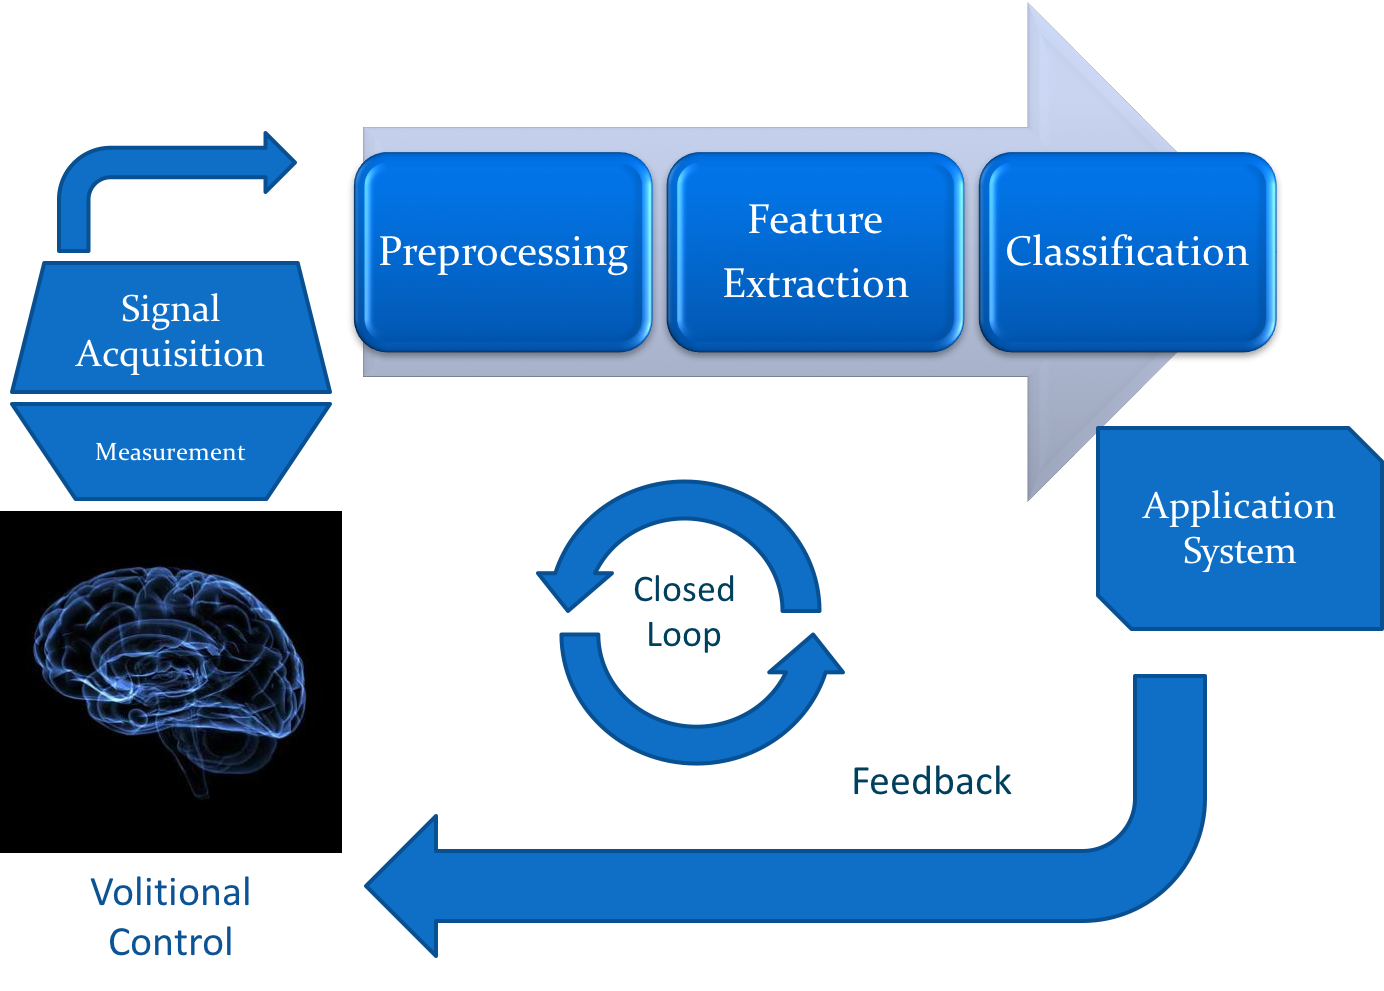
\includegraphics[scale=0.5]{images/bcichart.png}
\caption[BCI Block Diagram]{General components of a BCI system.}
\label{fig:bciblockdiagram}
\end{figure}

The basic model of any BCI is to take a multichannel digital signal $\mathbf{x}(n)$, and transform it to an output control signal $y(n)$ which can be a scalar or binary function.  The BCI system can be modeled as the transformation $T$.

\begin{equation}
y(n) = T\left[\mathbf{x}(n)\right]
\label{eq:bcimodel}
\end{equation}

What a BCI system must do, is to take at least a single bit of information out of $y(n)$ and use that information to derive some action. 

\section{Signal Processing}

From this signal processing point of view, BCIs are:

\begin{itemize}
\item Causal:  $ y(n) = f( \mathbf{v}(m) ) $, where $ m \leq n $.  The action of a BCI system depends on the history of the captured brainwaves.
\item Dynamic: $ y(n) = f( \mathbf{v}(m),  \mathbf{\dot{v}}(m),\mathbf{\ddot{v}}(m),...) $.  A BCI system is dynamic, where the output function do not depend only on the current value being observed, it does depend on its dynamic interactions.
\item Time invariant: $ y(n) = T\left[ \mathbf{v}(n) \right] \Rightarrow y(n-k) = T\left[ \mathbf{v}(n-k) \right] $.  The output of a BCI system does not depend on the particular time frame where it is being used.  However, Adaptive BCI, which do adapt to the user behavior are in general time variant.
\item Nonlinear: a system is linear when $T\left[ a_1 \mathbf{v}(n) + a_2 \mathbf{v}(n) \right]  = a_1 T \left[ \mathbf{v}(n) \right] + a_2 T \left[ \mathbf{v}(n) \right] $. Due to brainwave complexity, BCI systems are not linear.
\item Multirate or broadband \cite{Miller2010}:  The energy of brainwave spectrum is not confined to a certain band, and almost all frequency channels convey some information.
\end{itemize}

There are several filters that can be applied to the system to eliminate artifacts, enhance the signal, and to ease the detection of the discriminative information.

\textbf{Static Filters} like square or logartihmic were traditionally used in analog signal processing and are currently already embedded in the measuring device.  Wiener and Kallman Filters are usually applied to invasive techniques~\cite{NeuralEngineeringBookBinHe}.  The filter, particularly when it is linear, can be viewed as the matrix $M$ in:

\begin{equation}
y(n) = M T\left[\mathbf{x}(n)\right]
\label{eq:filters}
\end{equation}

\textbf{Spatial filters} are carefully adapted to the arrangement of sensors around or within the head and they emphasize the spatial structure of the information that is being captured. Derived from neuroscience research, locations on the head are structured according to neuroanatomical planes or axes and normally the brain, or the head, are divided in different anatomical regions (Figure \ref{fig:neuroanatomy}).   

\textbf{Spectral Filters}, on the other hand, do consider brainwaves as another digital signal, and they perform different transformations based on the spectral information contained within the signal $\mathbf{x}(n)$.  They can be combined and aggregated creating  \textit{Filter Banks} to enhance signal quality. 


\begin{figure}[htb]
\centering
\subfigure[Neuronal Planes]{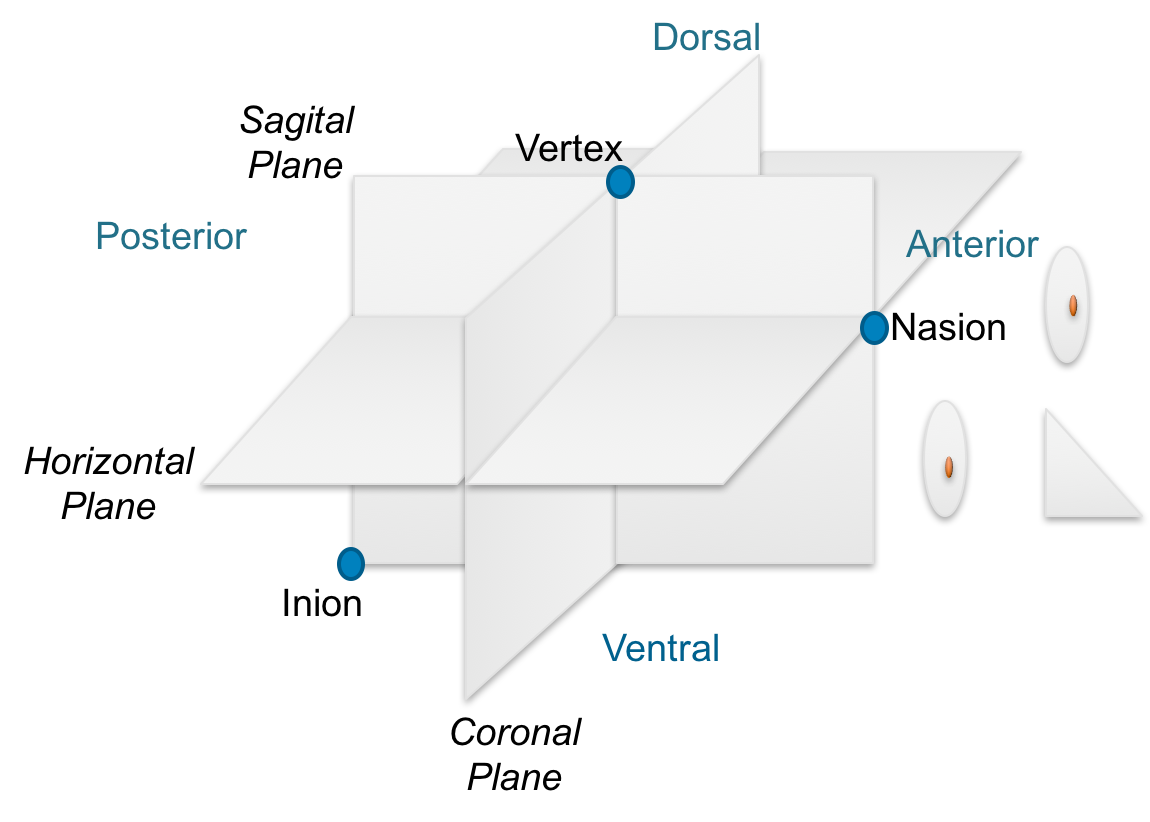
\includegraphics[scale=0.4]{images/neuralplanes.png}}
\subfigure[Neuroanatomical regions of the brain.]{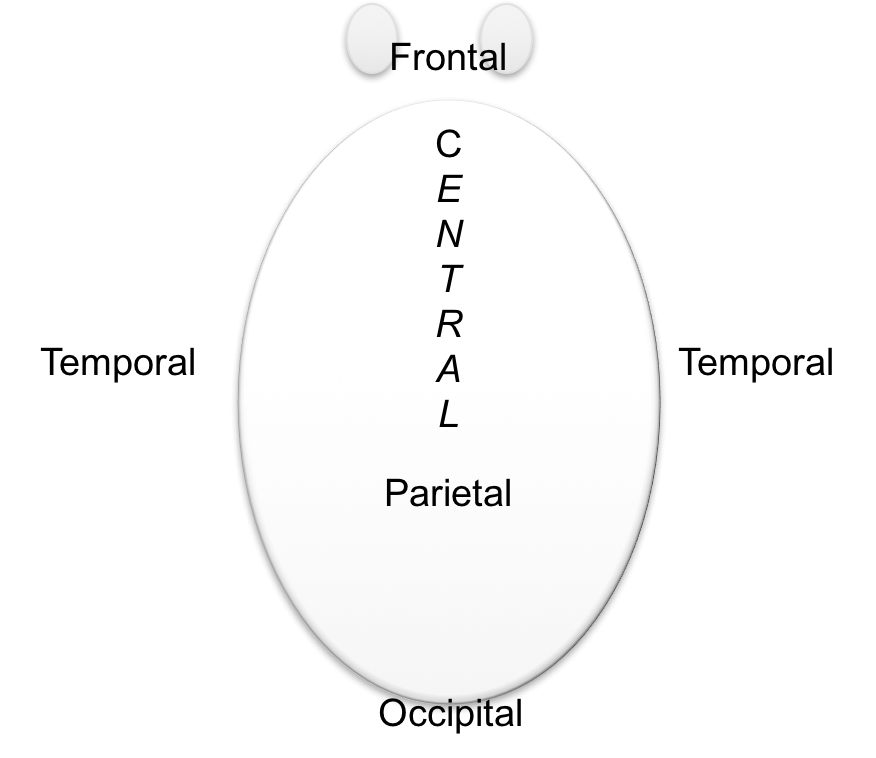
\includegraphics[scale=0.4]{images/neuroanatomy.png}}
\caption[Neuroanatomical structures of the brain]{Neuronal Planes regularly used in neuroscience research.  In BCI they are used to understand electrode location and spatial filters.}
\label{fig:neuroanatomy}
\end{figure}

%\begin{figure}[]
%\centering
%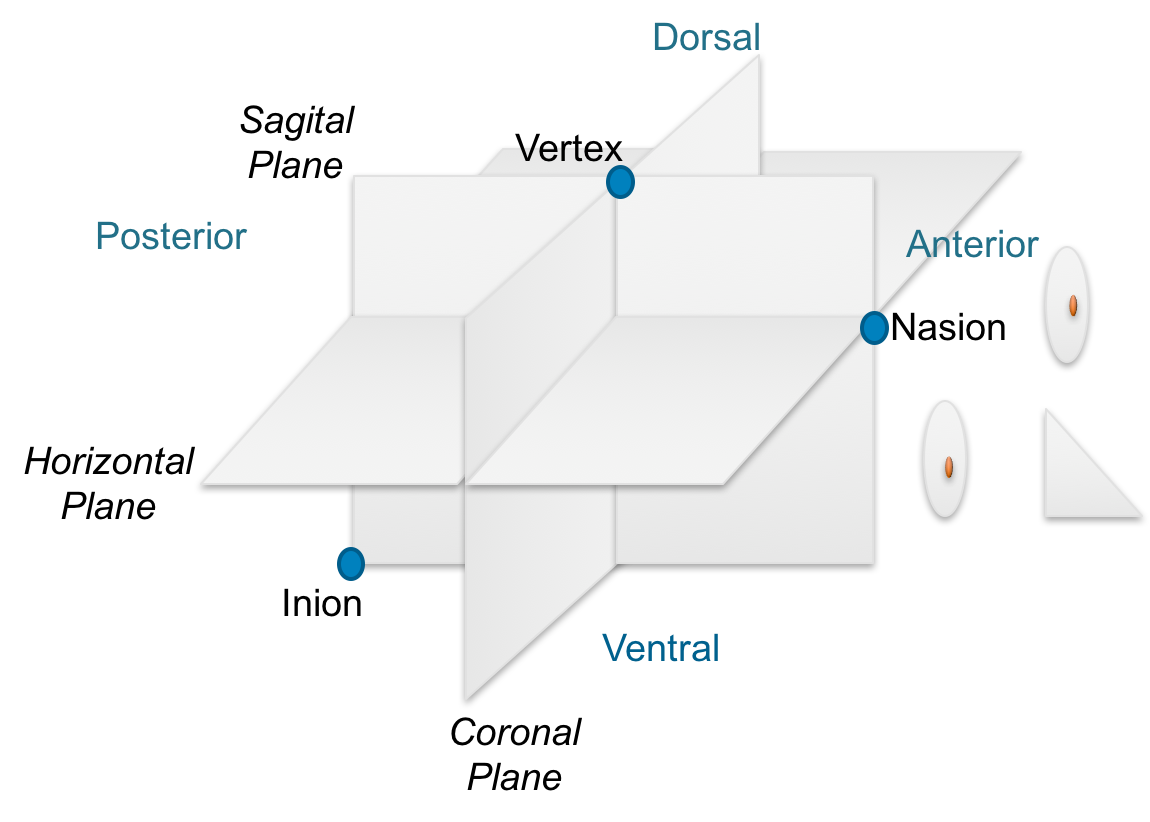
\includegraphics[scale=0.5]{images/neuralplanes.png}
%\caption[Neural Planes]{Neuronal Planes regularly used in neuroscience research.  In BCI they are used to understand electrode location and spatial filters.}
%\label{fig:neuralplanes}
%\end{figure}
%
%\begin{figure}[]
%\centering
%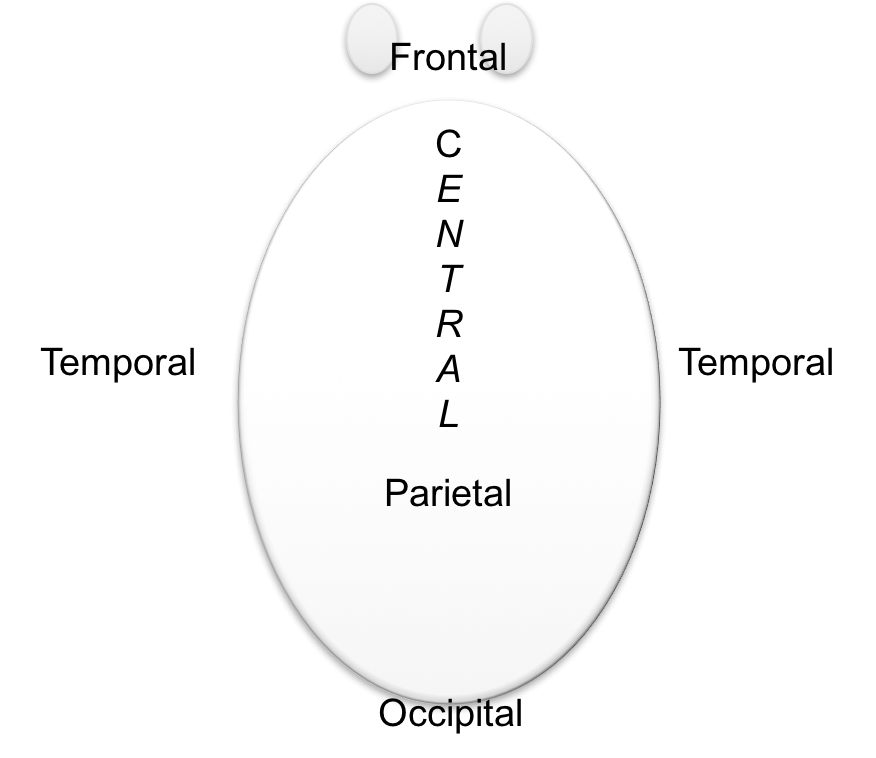
\includegraphics[scale=0.5]{images/neuroanatomy.png}
%\caption[Neuroanatomy]{Neuroanatomical regions of the brain.}
%\label{fig:neuroanatomy}
%\end{figure}

\section{The Forward and Inverse Model}

Brainwaves are obtained via sensors. Each one of them captures only a part or a version of the information.  However, whatever is actually happening inside the brain can be only recovered indirectly from the \textit{Sensor Space}. From there, the information can be traced back to the real landscape where the information source is located, inside the \textit{Source Space}.  This is a regular problem found in Engineering and it is not different in BCI.  \textit{Calculating} the signal on each a sensor from a projection of a known source of information from within the head is called \textit{The Forward Problem}\cite{Parra2008,WolpawJonathanR2012}  and doing the opposite, \textit{estimating} the contributions of different sources to whatever activity is found on sensors is called  \textit{The Inverse Problem} .  The latter is more relevant in BCI because it allows to determine source origins that can be mapped more directly to cognitive activities.  However, this kind of problem is highly ill-posed and it is precisely where the majority of the efforts of this discipline are concentrated due to its complexity.

Particularly for noninvasive electrophysiological modalities, an additional problem makes things harder.  Due to its electromagnetic properties, the brain acts like conductive gel, and any signal that is generated inside the brain is irradiated to every direction and it can influence every sensor regardless of its position.  This is called \textit{Volume conduction} \cite{Nam2018,Buzsaki2012} and can be visualized in Figure~\ref{fig:volconduction}.

\begin{figure}[]
\centering
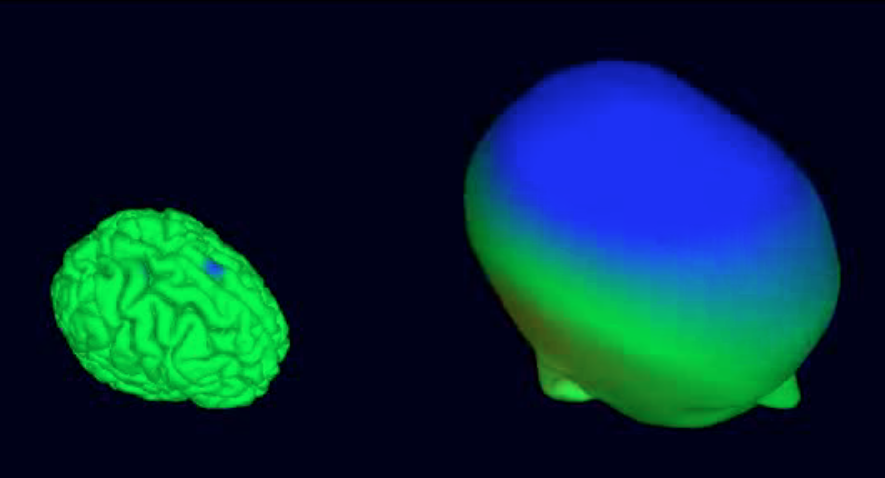
\includegraphics[height=6cm,width=14cm]{images/volconduction1.png}
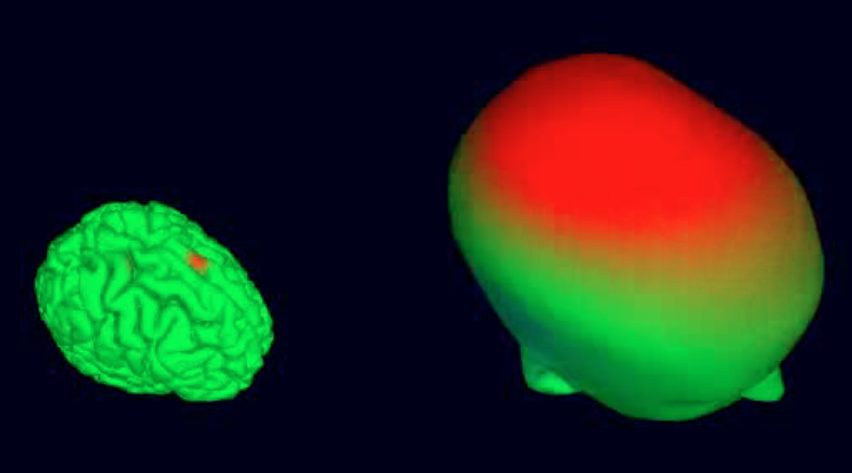
\includegraphics[height=6cm,width=14cm]{images/volconduction2.png}
\caption[EEG Volume Conduction]{A source signal with positive/negative polarity is generated in a very specific region of the brain but due to volume conduction their influence affects a widespread area of the scalp where sensors are located (Image from Swartz Center for Computational Neuroscience) }
\label{fig:volconduction}
\end{figure}

\section{Brain Imaging Technologies}

The measuring technique determines the most important taxonomic differentiation in BCI, according to how they extract the information from the CNS.

\begin{enumerate}
\item fNIRS: functional Near Infra Red Spectroscopy.
\item EEG: Electroencephalography
\item MEG: Magnetoencephalography
\item PET: Positron Emission Tomography
\item fMRI: functional Magnetic Resonance Imaging
\item ECoG: Electrocorticography 
\item INR: Intracortical Neuron Recordings.  Particularly LFP (iEEG, intracraneal EEG\cite{Buzsaki2012}) and microelectrodes (Utah array).
\end{enumerate}

ECoG and INR are invasive technologies that require some neurosurgery and an implantation of electrodes inside the skull the former, and inside the brain the latter.  All the remaining imaging techniques are external or noninvasive.  Hybrid BCI, or Brain Neural Computer Interface, are BCI devices that use not only signals from the CNS, they utilize any kind of available biosignal that can be volitionally modulated to transmit information (this is called dependant BCI).  On the other hand, when the pace of the BCI is regulated by external stimulus it is called synchronous and when the user choose their own pace to transmit information, it is often called asynchronous or self-paced BCI.

Recent years have seen an incredible advance of Passive BCI, pBCI \cite{Zander2010}.  The original definition of BCI did not include Passive modalities but per definition \ref{def:BCI} it is now part of this discipline.  The important aspect is that passive technologies do not entail necessary the volitional requirement to transmit information.  EEG-based passive BCI is a promising and advancing area of research and of commercial applications.

\section{Electroencephalography}

Above all, Electroencephalography (EEG), is the most widespread method to gather information from the CNS in a non-invasive way. They are of particular interest in BCI mainly because of their non-invasiveness, their optimal time resolution and acceptable spatial resolution. Moreover, they are portable, cheap, wearable and can be more easily integrated into fashionable designs aimed for real users, which prefer cap-like devices~\cite{Huggins2015}. 

The Electroencephalography consists on the measurement of small variations of electrical currents over the scalp.  This represents the summed activity of post-synaptic potentials PSPs of pyramidal neurons located perpendicular to the scalp~\cite{Nam2018}. Only one percent of synchronized activity of pyramidal neurons are stronger that the remaining desynchronized neurons~\cite{Schomer2010} and explain ninety-nine percent of the signals obtained from EEG.  This brain imaging technology is one of the most widespread used methods to capture brain signals and was initially developed by Hans Berger in 1924 and has been extensively used for decades to diagnose neural diseases and other medical conditions.

%Routinely physicians explore morphologically these raw EEG signals scavenging for signs of disease or irregular patterns and they have been doing this since almost the dawn of the technology at the hands of Hans Berger. Sleep spindles, Lambda waves, K-Complexes, Vertex waves, Positive Occipital Sharp Transients and more visual features had been identified with relevant clinical characterizations [16]. Even within the BCI community, visually extracting artifacts for offline processing is a common and well known practice [1,11]. 

%The EEG signal goes from 10-100 microvolts
%monopolar, reference, averaged, 
%bipolar
%segmentation is commong, which is generally called epoching
%trials are general realizations of the experiment.
%tampering window could be gaussian, hamming, blackman, hanning
%Impedance

The first characterization that Dr. Berger detected was the Visual Cortical Alpha Wave, the \textit{Berger Rythm} \cite{Jansen1991}.  He understood that the amplitude and shape of this rhythm was coherently associated to a cognitive action (eyes closing).  
We should ask ourselves if the research advancement that came after that discovery would have happened if it weren't so evident that the shape alteration was due to a very simple and verifiable cognitive process.

The EEG signal is a highly complex multi-channel time-series.  It can be modeled as a linear stochastic process with great similarities to noise \cite{Thakor2004}.  It is measured in microvolts, and those slightly variations are contaminated with heavy endogenous artifacts and exogenous spurious signals.  
 
\begin{figure}[]
\centering
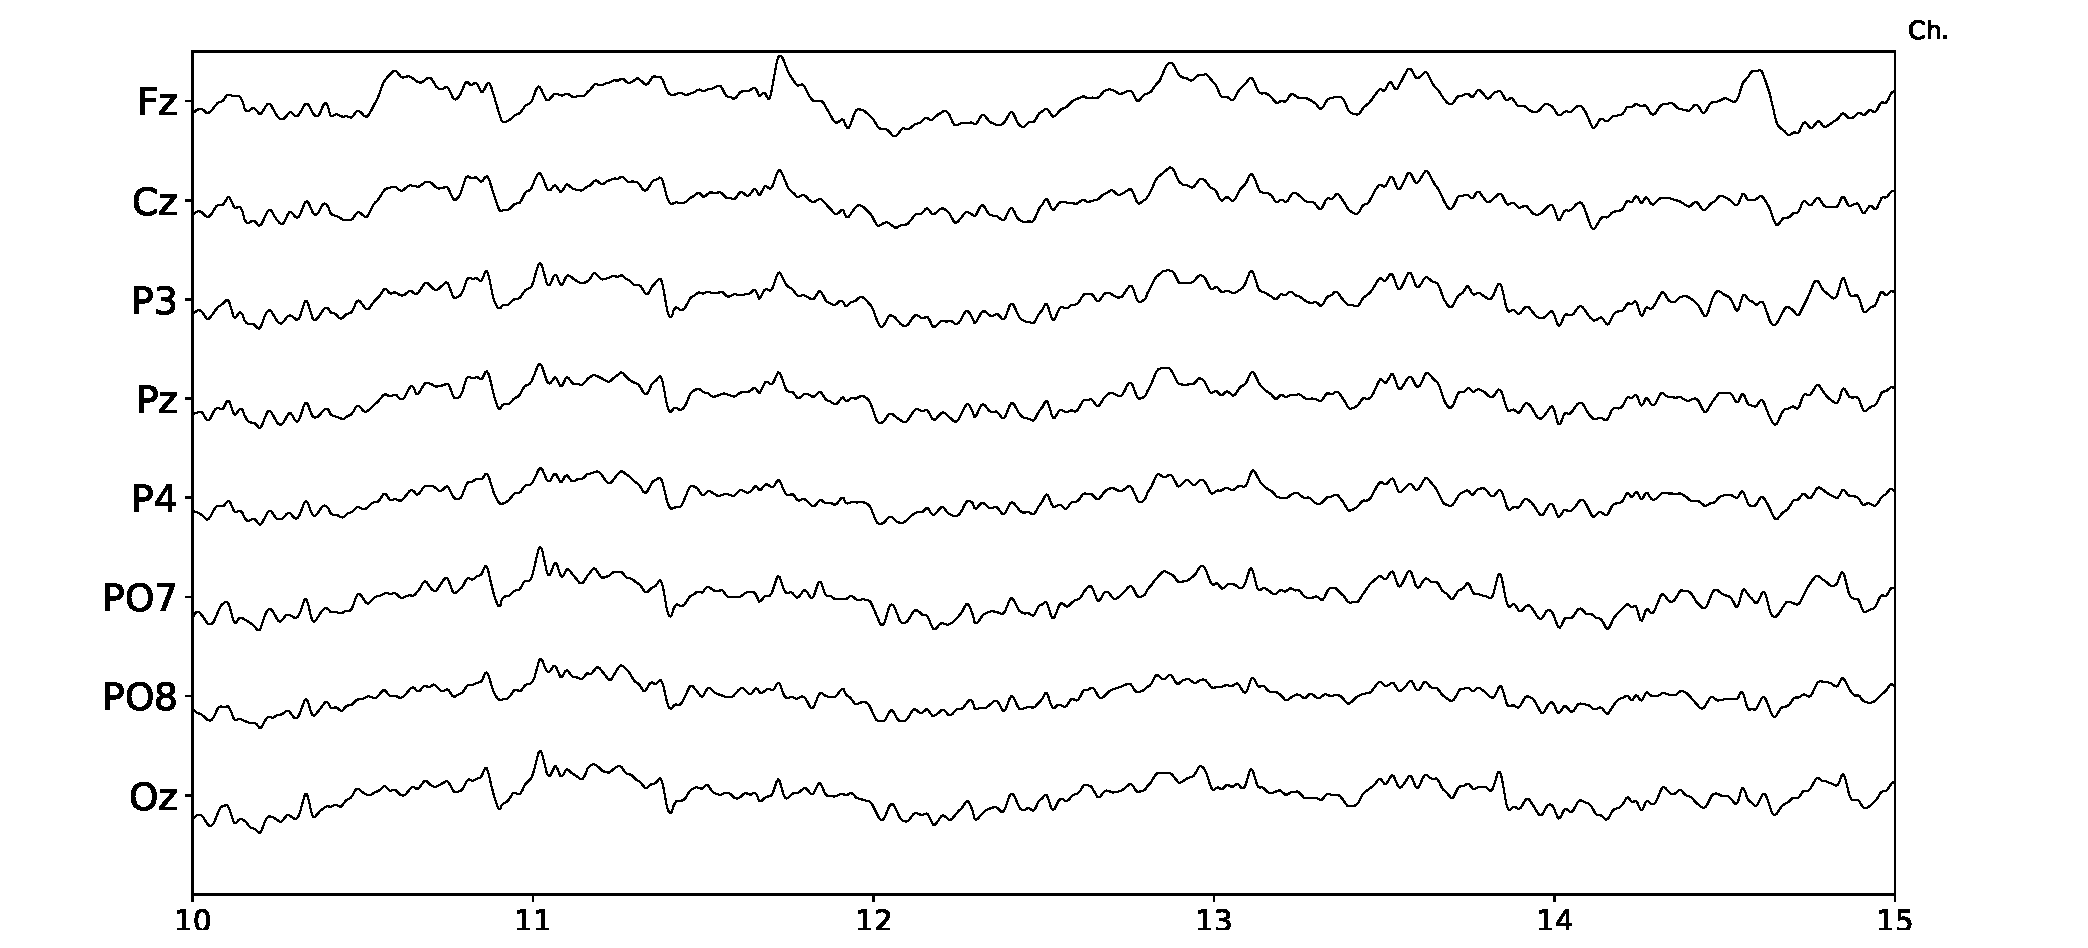
\includegraphics[height=6cm,width=14cm]{images/sampleeeg.eps}
\caption[Sample Multichannel EEG signal]{Sample EEG signal obtained from (g.Nautilus, g.Tec, Austria). Time axis is in seconds and five seconds are displayed.  The eight channels provided by this device are shown.}
\label{fig:sampleeeg}
\end{figure}


\begin{figure}[]
\centering
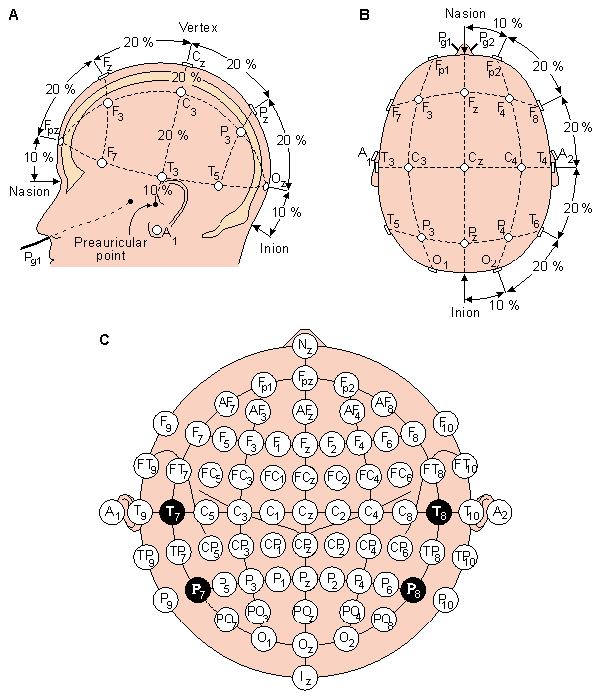
\includegraphics[height=6cm,width=6cm]{images/ElectrodePositions1020.png}
\caption[Electrode Locations]{International 10-20 system that standardize electrode locations over the scalp.}
\label{fig:electrodelocations}
\end{figure}

%locations.eps

The device that captures these small variations in current potentials over the scalp is called the Electroencephalograph (Figure \ref{fig:digitalelectroencephalograph}).  Electrodes are located in predetermined positions over the head, usually embedded in saline solutions to facilitate the electrophysiological interface and are connected to a differential amplifier with a high gain which allowed the measurement of tiny signals. Although initially analog devices were developed and used, nowadays digital versions connected directly to a computer are pervasive.  A detailed explanation on the particularities and modeling of EEG can be obtained from \cite{Jackson2014}, and a description of its electrophysiological aspects from \cite{Haberman2012}.

\begin{figure}[]
\centering
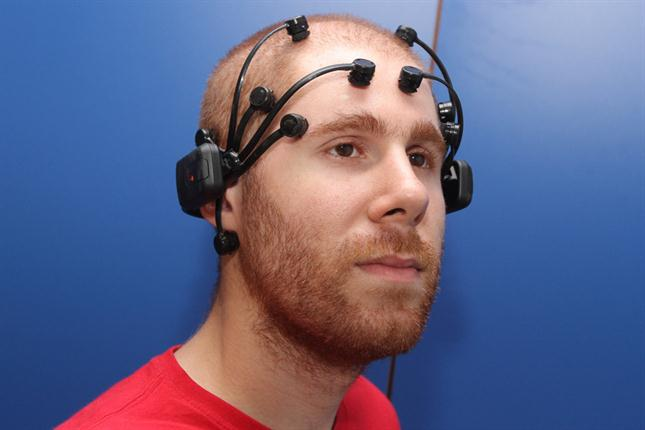
\includegraphics[height=4cm,width=7cm]{images/emotivsubject.jpg}
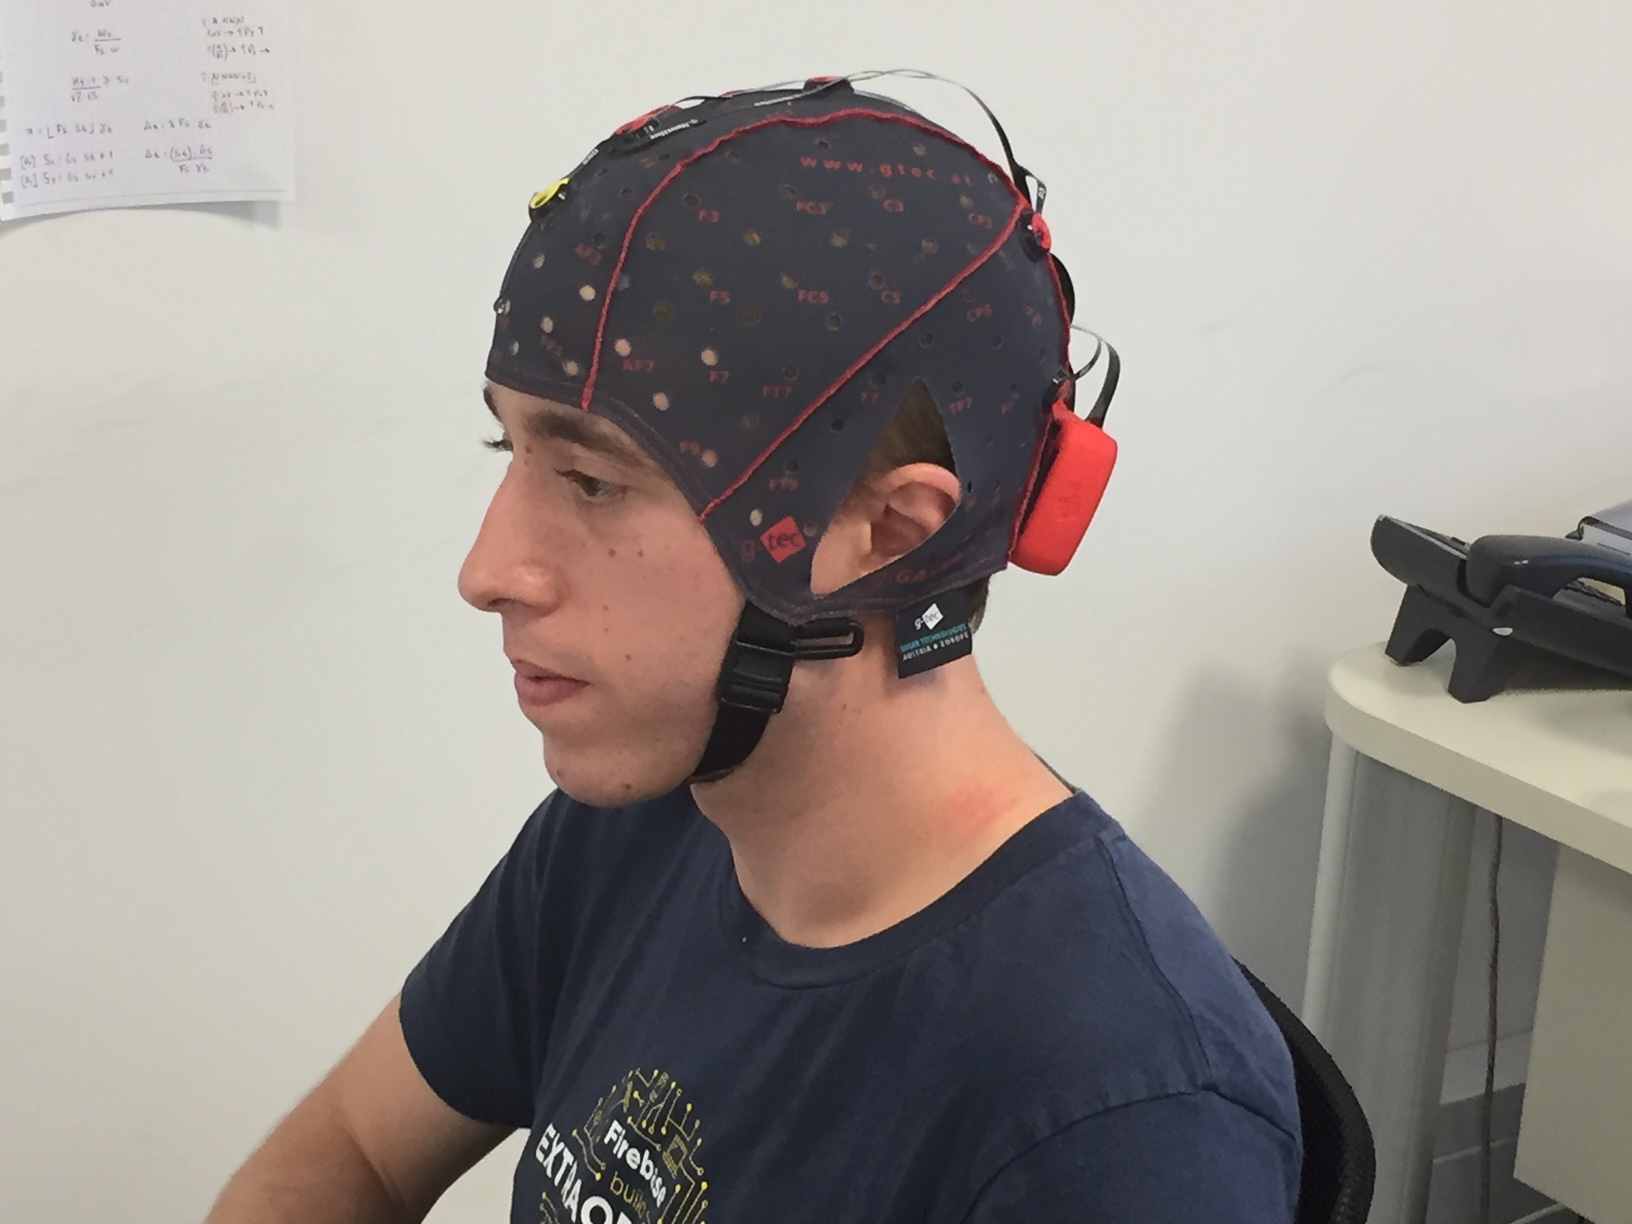
\includegraphics[height=4cm,width=7cm]{images/gTecsubject.jpg}
\caption[Wearable portable Digital Electroencephalograph]{Consumer-grade digital electroencephalograph.}
\label{fig:digitalelectroencephalograph}
\end{figure}


Overall, EEG signals can be described by their phase, amplitude,  frequency and \textit{waveform}.  The following components regularly  characterize EEG signals:

\begin{itemize}
\item Artifacts:  These are signal sources which are not generated from the CNS, but can be detected from the EEG signal.  They are called endogeneous or physiological when they are generated from a biological source like muscles, ocular movements, etc., and exogeneous or non-physiological when they have an external electromagnetic source like line induced currents or electromagnetic noise\cite{Weeda2012}.  Ambulatory studies or out-of-the lab studies introduces artifacts that are derived from the person movement from the FES and also from other devices in hybrid BCI, or multi-modal BCIs.
\item Non-Stationarity: the statistical parameters that describe the EEG as a random process are not conserved through time, i.e. its mean and variance, and any other higher-order moments are not time-invariant \cite{Jansen1991}.
\item DC drift and trending: in EEG jargon, which is derived from concepts of electrical amplifiers theory, Direct Current (DC) refers to very low frequency components of the EEG signal which varies around a common center, usually the zero value.  DC drift means that this center value drifts in time.  Although sometimes considered as a nuisance that needs to get rid of, it is known that very important cognitive phenomena like Slow Cortical Potentials or Slow Activity Transients in infants do affect the drift and can be used to understand some particular brain functioning \cite{Schomer2010}.
\item Basal EEG activity: the EEG is the compound summation of myriads of electrical sources from the CNS.  These sources generate a baseline EEG which shows continuous activity with a small or null relation with any concurrent cognitive activity or task.
\item Inter-subject and intra-subject variability: EEG can be affected by the person's behavior like sleep hygiene, caffeine intake, smoking habit or alcohol intake previously to the signal measuring procedure \cite{Farzan2017}.
\end{itemize}

Regarding how the EEG activity can be related to an external stimulus that is affecting the subject, it can be considered as

\begin{itemize}
\item Spontaneous: generally treated as noise or basal EEG.
\item Evoked: activity that can be detected synchronously after some specific amount of time after the onset of the stimulus.  This is usually referred as time-locked.  In contrast to the previous one, it is often called Induced activity.
\end{itemize}

\noindent Additionally, according to the existence of a repeated rhythm, the EEG activity can be understood as

\begin{itemize}
\item Rhythmic: EEG activity consisting in waves of approximately constant frequency.  It is often abbreviated RA (regular rythmic activity). They are loosely classified by their frequencies, and their naming convention was derived from the original naming used by Hans Berger himself:

\begin{itemize}
\item Alpha Waves (10 Hz)
\item Delta (0-4 Hz)
\item Theta (4-8 Hz)
\item Sigma (12-16 Hz)
\item Beta (12-30 Hz)
\item Gamma (30-100 Hz)
\item Omega (60-120 Hz)
\item Rho (250 Hz) hippocampal
\item Sigma Thalamocortical burst (600 Hz)
\end{itemize}

\item Arrhythmic: EEG activity in which no stable rhythms are present.  
\item Dysrhythmic: Rhythms and/or patterns of EEG activity that characteristically appear in patient groups and rarely seen in healthy subjects.
\end{itemize}

The number of electrodes and their positions over the scalp determines a Spatial Structure: signal elements can be generalized, focal or lateralized, depending on in which channel (i.e. electrode) they are found.

%Finally, indexes can be derived as  CFC, Cross Frequency Coupling,  Phase-Amplitude Coupling, Phase-Phase Coupling.


\section{BCI EEG Paradigms}

%Due to their popularity ($71.2\%$ of the BCI projects submitted to BCI Award 2016 were with EEG) BCI based on EEG are 

\textit{BCI Paradigms} are referred to noninvasive EEG-based BCI configurations that can be used to transmit volitional information.  The popularity of EEG ($71.2\%$ of the BCI projects submitted to BCI Award 2016 were with EEG)~\cite{Guger2017} pushed the adoption of paradigms exclusively for noninvasive BCI.   Their chronology can be found in Figure \ref{fig:story}. They are

\begin{enumerate}
\item Steady State Visual Evoked Potentials
\item Bereitschaftspotentials, Readiness Potential or Movement-Related Potentials
\item Motor Imagery
\item ERD/ERS: Event Related
\item Wadsworth BCI
\item Graz BCI
\item Selective Attention
\item P300
\item N400
\item Mental Tasks
\item Operant Conditioning
\item Slow Cortical Potentials
\item Berlin BCI


\end{enumerate}


\section{State of the Art of BCI Algorithms for EEG processing}

According to general layout of any BCI, Figure \ref{fig:bciblockdiagram}, specific algorithms or techniques are derived for both the Feature extraction and classification step.

The most relevant features used in BCI are:

\begin{itemize}
\item Time points:  the sequence of time series, often, concatenated in time or space.
\item Band Power: frequency based features.
\item Complexity:  based on complexity measurements like entropy, fractal.
\item Statistical: AR parameters, covariances matrix.
\end{itemize}

The most successfull used and verified classification methods for BCI \cite{Lotte2007} can be described as linear versions of popular Machine Learning tools.  Particularly, Support Vector Machines SVM, Linear Discriminant Analysis LDA and its variant SWLDA.  This one was also relevant for two reasons:  the first is that the stepwise identification of features improves the selection criteria and also the spatial filter that this procedure encompass.  Additionally, and more from a more pragmatic perspective, this method was included in the popular BCI2000~\cite{Schalk2004} package and was the default option for anyone doing ERP identification.  Spatial Filters have also being incorporated and have shown substantial improvement in classification accuracies.  The now classical Common Spatial Patterns CSP for the identification of Motor Imagery as well as the xDAWN algorithm for P300 identification.

Recent years (circa 2018) have seen the evolution of the methodology but the focus was not centered on any particular classification algorithm.  Instead how they are used became much more important~\cite{Lotte2018}.

\begin{itemize}
\item Ensemble Classifiers: SVM ensembles~\cite{Rakotomamonjy2008} and variants of Random Forest~\cite{Steyrl2015}.  Features are segmented and divided and the forest performs a classification step on each part and maximizes classification accuracies.
\item Cross-Paradigm BCI: the use of Reinforced Signal RS with ErrP feedback or the use of SSVEP in combination with P300 detection~\cite{Lotte2018}.
\item Adaptive Classifiers: the parameters of the classifiers are adapted continuously and online adapting to the natural variation of the EEG signals~\cite{Lotte2018}.
\item Transfer Learning: transfer the calibration information obtained by users to new subjects.  This aims to eases the issue of the intra-subject variability in BCI .
\item RGC: Rienmann Geometry Classifiers
\item Tensor-based BCI
\item Deep Learning: heavily tried but without significant success.
\end{itemize}

%What if we can find an automatic system to identify, search, and even classify EEG signals based on the morphological visual structure of the signal, mimicking what the physician does, but using automated tools to do so?

\section{EEG Waveform Analysis}

\subsection{EEG Waveform Characterization}

The shape of the signal, the waveform, can be defined as the graphed line that represents the signal's amplitude plotted against time. It can also be called EEG biomarker,  EEG pattern, motifs, signal shape, signal form and a morphological signal \cite{Jansen1991}.

The signal context is crucial for waveform characterization, both in a spatial and in a temporal domain \cite{Jansen1991}.  Depending on the context, some specific waveform can be considered as noise while in other cases is precisely the element which has a cognitive functional implication.

%aforegoing
%hitherto

%phenomenological, the signal is treated as a black box.

%Signal Morphology is not precisely defined in the literature but may refer to
%
%\begin{itemize}
%\item RA (regular rythmic activity) 
%\item low-voltage rapid activity 
%\item sharp waves
%\item longitudinal-bipolar and transverse- bipolar montages (Clinical EEG)
%\end{itemize}

A waveform can have a characteristic shape, a rising or falling phase, a pronounced plateau or it may be composed of ripples and wiggles. In order to describe them, they are characterized by its amplitude, the arch, whether they have (non)sinusoidal shape, by the presence of an oscillation or imitating a sawtooth (e.g. Motor Cortical Beta Oscillations).  The characterization by their sharpness is also common, particularly in Epilepsy, and they can also be identified by their resemblance to spikes (e.g. Spike-wave discharge).

Other depictions may include, subjective definitions of sharper, arch comb or wicket shape, rectangular, containing a decay phase or voltage rise, peaks and troughs, short term voltage change around each extrema in the raw trace.  Derived ratios and indexes can be used as well like peak and trough sharpness ratio, symmetry between rise and decay phase and slope ratio (steepness of the rise period to that of the adjacent decay period).  For instance,  wording like "Central trough is sharper and more negative that the adjacent troughs" are common in the literature.

Other regular characterizations which are based on shape features may include:

\begin{itemize}
\item Attenuation: Also called suppression or depression. Reduction of amplitude of EEG activity resulting from decreased voltage. When activity is attenuated by stimulation, it is said to have been "blocked" or to show "blocking".
\item Hypersynchrony: Seen as an increase in voltage and regularity of rhythmic activity, or within the alpha, beta, or theta range. The term suggest an increase in the number of neural elements contributing to the rhythm and a synchronization of neurons with similar firing patterns~\cite{Buzsaki2012}.
\item Paroxysmal: Activity that emerges from background with a rapid onset, reaching (usually) quite high voltage and ending with an abrupt return to lower voltage activity. 
\end{itemize}

\begin{itemize}
\item Monomorphic: Distinct EEG activity appearing to be composed of one dominant activity
\item Polymorphic: distinct EEG activity composed of multiple frequencies that combine to form a complex waveform.
\item Transient. An isolated wave or pattern that is distinctly different from background activity.
\end{itemize}


%\subsection{EEG Patterns}
%
%%The clinical EEG patterns are identified by the shape of waveform amplitude plotted against time.
%
%Non-exhaustive list of transient events
%Waveform characterization is of quite importance in terms of Event Related Potentials.  
%Determination of transient events, and particularly amplitude of different subcomponents, latency or even phase, has proved very importan concequences in terms of the different cognitive approach.
%
%%inverse problem is mathematically intractable Voytek 2009
%
%Oscillatory activity can also have their differente or distinctive waveforms.  Slow oscillations, which are assosiated with REM, sawtooth-shaped.
%Sleep spindles can also be considered oscilations and they have a distintinc form assosiated with stage 2 dream.
%Visual Cortical alpha and rolandic central mu waves arch-like structure (similar to the greek letter mu).  Slope Ratio.  Trough voltage remains contstant while peak voltage fluctuates.   Steep slopes,   Amplitude asymmetry 
%ponto-geniculo-occipital
%(PGO) waves.
%Rhythms in neural activity are observed across various temporal and spatial scales and are often
%referred to as oscillations (see Glossary) [1]. Traditionally, neural oscillations have been
%clustered into canonical frequency bands, including delta (1–4 Hz), theta (4–8 Hz), alpha (8–
%12 Hz), beta (15–30 Hz), gamma (30–90 Hz), and high gamma (>50 Hz). These bands roughly
%correspond to frequency ranges commonly observed in human electroencephalography (EEG)
%studies. Although they have been observed for nearly a century, recent theories suggest that
%these oscillations play an active role in neural communication.  Hippocampal theta oscillations, for example, are among the best-studied rhythms in the local field potential (LFP); they have a stereotyped sawtooth shape. In sleep research sleep 2 stage the background of KComplex and sleep spindles is theta waves
%
%%by application to Brain Computer Interfaces or EEG diagnosis (BCI a review, BCI Vidal 1973)
%
%
%
%%(e.g. FIRDA - Frontal Intermittent Rhythmic Delta) and posteriorly in children e.g. OIRDA - Occipital Intermittent Rhythmic Delta).
%
%%alpha dissapears when alerting by any mechanism (thinking, calculating)
%
%a) Spike: a transient with a pointed peak and a duration from 20 to under 70 msec.
%b) Sharp wave: a transient with a pointed peak and duration of 70-200 msec.
%
%Some initial works on EEG explored the idea to extend human capacities analyzing EEG waveforms  (automatic detection of k complexes), (A Waveform Analyzer Applied to the Human EEG) where a feature from amplitude and frequency of its signal and its derivative in time-domain is used.  Althought CASENET REFERENCe explored "waveform" structure they were purely based on spike detection based on feeding artificial neural networks.  
%
%ACA VA EL RESTO DE LOS METODOS (fujimori, PAA, etc).  Uchida 1999

The traditional clinical approach consists in analyzing the paper strip that is generated by the plot of the signal obtained from the device.  Expert technician and physicians analyze visually the plots looking for specific patterns that may give a hint of the underlying cognitive process or pathology.   Atlases and guidelines were created in order to help in the recognition of these complex patterns.   Even Video-electroencephalography scalp recordings are routinely used as a diagnostic tools \cite{Giagante2003} .  The clinical EEG research has also focused on temporal waveforms, and a whole branch of electrophenomenology has arisen around EEG \textit{graphoelements} \cite{Schomer2010}.  

Sleep Research has been studied in this way by performing Polysomnographic recordings (PSG)  \cite{Rodenbeck2006}, where the different sleep stages are evaluated by visually marking waveforms or graphoelements in long-running electroencephalographic recordings, looking for patterns based on standardized guidelines.   Visual characterization includes the identification or classification of certain waveform components, or transient events, based on a subjective characterization (e.g. positive or negative peak polarity) or the location within the strip.  It is regular to establish an amplitude difference between different waveforms from which a relation between them is established and a structured index are created (e.g. sleep K-Complex is well characterized based on rates between positive vs negative amplitude) \cite{Uchida1999}.  Other relevant EEG patterns for sleep stage scoring are alpha, theta, and delta waves,  sleep spindles, polysplindles, vertex sharp waves (VSW), and sawtooth waves (REM Sleep).

Moreover, EEG data acquisition is a key procedure during the assessment of patients with focal Epilepsy for potential seizure surgery, where the source of the seizure activity must be reliably identified. The onset of the Epileptic Seizure is defined as the first electrical change seen in the EEG rhythm which can be visually identified from the context and it is verified against any clinical sign indicating seizure onset.  The interictal epileptiform discharges (IEDs) are visually identified from the paper strip, and they are also named according to their shape: spike, spike and wave or sharp-wave discharges\cite{EEGIntro}.  

%Seizures captured in their entirety typically show progression from low-voltage, high-frequency spikes to high-voltage, low-fre- quency spike-and-slow wave activity, before stopping abruptly and being replaced by background slowing or suppression (Fig. 29.9). Usual morphologic features include typical rhythmic, gen- eralized, symmetric spike-and-waves or polyspikes and waves at 2 to 3.5 Hz; atypical spike and wave with lower frequency and less symmetry; multiple spike-and-wave (repetitive complexes of two or more spikes followed by a slow wave); and high-voltage, repetitive, rhythmic, focal or generalized delta activity with inter- mixed spikes, sharp waves, or sharp components (Fig. 29.24) (45). Diagnosis is more difficult when the seizure (or SE) pre- cedes the beginning of the tracing and continues beyond its end. In such cases, rhythmic sharp features, typically faster than 1 Hz, may be seen, often with variability.

%Finally, there are specific EEG patterns that can be used to determine Depth of anestisia. 

%The waveform of the EEG depends on the settings of the capturing device.  The most important part to consider is that of montage.  It could be bipolar or referencial.  The traditional convention, somehow maintained in neuro research, downward polarity was considered negative and upward deflection for negative (Knott, 1985)  It is of utmost importance to remark that  EEG waveforms represent the differential voltage between a given electrode and the recording reference. It is therefore clear that the choice of reference completely determines EEG waveforms (Lehmann, 1987; Dien, 1998), an important methodological consideration that all too often is still not recognized in the EEG literature. For example, recording with a vertex (Cz) reference would lead to small EEG deflections in the proximity of Cz due to potential synchronization of firing activities within closely spaced brain regions and volume propagation of the EEG signal. Similarly, recording with mastoid or linked ears montage would lead to rather small waveforms at electrodes positioned over temporal brain regions (Pivik et al., 1993). Digital EEG can be rereferenced offline.  

%
%BCI --> distinguishing the pertinent signal characteristics from extraneous content and representing them in a compact or menaingful form, amenable to interpretation by a human or computer (Wolpaw and Wolpaw)

%Transient phenomena allows also to record occurrence and temporal sequence (mimicking spike analysis in neuro reserach)

%The traditional approach do not consider waveform even though the brain oscilations are in general nonsinusoidal (reference)
% Waveform characterization, on the other hand, has been extensively used in artifact detection and averaging.

\subsection{EEG Waveform Analysis Algorithms}

Shape or waveform analysis methods are considered as nonparametric (in opposition to statistical or dynamical models).  They explore signal's time-domain metrics or even derive more complex indexes from it \cite{Thakor2009}. 

One of the earliest approach to automatically process EEG data is the Peak Picking method.  Although of limited usability, peak picking has been used to determine latency of transient events in EEG \cite{Jaskowski2000,Zhang2011}.  Straightforward in its implementation, it consists in selecting a component, a simple component based on the expected location of its more prominent deflection \cite{Ouyang2017}.  Evoked Potentials (EPs) and Event Related Potentials (ERPs) are transient component that may arise as a brain response to an external visual, tactile or auditory stimulus.  Particularly, EPs are regularly used to assess auditory response in infants. ERPs are precisely characterized in this manner, where the name of many of the EEG features evoke directly a peak within the component, e.g. P300 or P3a, P3b or N100.  This leads to a natural procedure to classify them visually by selecting appropriate peaks and matching their positions and amplitudes in an orderly manner.  The letter provides the polarity (Positive or Negative) and the numbering shows the time referencing the stimulus onset, or the ordinal position of each peak (first, second, etc).   

A related method is used in \cite{Alvarado-Gonzalez2016} where the area under the curve of the EEG is sumarized to derive a feature.  This was even used in the seminal work of Farwell and Donchin on P300 \cite{Farwell1988,WolpawJonathanR2012}. Additionally, a logarithmic graph of the peak-to-peak amplitude which is called amplitude integrated EEG (aEEG) \cite{Shah2015} is used nowadays in Neonatal Intensive Care Units.

Other works on EEG explored the idea to extend human capacities analyzing EEG waveforms \cite{Klein1976} where a feature from the amplitude and frequency of its signal and its derivative in time-domain is used.  Moreover, other works explored the use of Mathematical Morphology \cite{Yamaguchi2009}, where the time-domain structure of contractions and dilations were studied. Finally the proposals of Burch, Fujimori, Uchida and the Period Amplitude Analysis (PAA) \cite{Uchida1996} algorithm are few of the earliest proposals where the idea of capturing the shape of the signal were established.

%Althought CASENET REFERENCe explored "waveform" structure they were purely based on spike detection based on feeding artificial neural networks.  

 %(fujimori, PAA, etc).  Uchida 1999

%\subsubsection{Averaging Methods}
%
%The methods that allow to identified waveforms are used to determine different alignments while averaging epochs.
%
%This long-standing problem has been tackled from different perspectives.  Woody's Template Matching is perhaps the best effort as well as Pham, and Tuan and others EML.
%
%Dictionary, template based method.  Many do not consider the waveform, albeit they do use a set of templates obtained from a dictionary.
%
%Cross Covariance with Template or Cross Correlation or ACF: Autocorrelation Function: PHAM METHOD
%
%Applying a FIR filter with templates 
%
%Krusienski et al 2007
%Serby et al 2005
%
%extended to wavelent analysis.
%
%Dynamic Time Warping and other Warp Averaging methods were also used.
%
%Wrapping Analysis
%
%Warp averaging

%Where are the waveforms ? By estimates from the 2016 BCI Award, around 71.2$\%$ of noninvasive BCI research is based on Electroencephalography (EEG) [1]. Although mature clinical EEG has traditionally focused on temporal waveforms, and a whole branch of electrophenomenology has arisen around EEG graphoelements [2], signal analysis methods which follow this path has been overshadow in BCI research. Few works have investigated the idea of exploiting signal waveforms to analyze the EEG signal on BCI applications. The seminal work of Bandt-Pompe Permutation Entropy [3] explores succinctly this concept and in [4] an approach based on Slope Horizontal Chain Code is presented. A similar methodology is implemented in [5] based on Mathematical Morphological Analysis. The work proposed here is based on waveform analysis of the shape of the EEG signal, but using the histogram of gradient orientations, mimicking what traditionally electroencephalographers have been doing for almost a century: visually inspecting raw EEG signal plots. Material, Methods and Results: The histogram of gradient orientations is a popular and powerful tool used in Computer Vision to characterize local features from images and is the basis of the feature generation algorithm in Lowe's SIFT Descriptor [7]. This technique can be applied to identify components in EEG signals in five steps, (1) signal preprocessing, (2) signal segmentation, (3) transformation on a channel by channel basis of each signal segment into a binary image of a signal plot, (4) assignment of keypoint location on the newly created image depending on the physiological phenomena under study and finally (5) calculation of the histogram of gradient orientations using finite differences from the image around the keypoint (Figure 1). This method generates a feature, a normalized 128-dimension SIFT descriptor, which can be used to compare the signal segments that were used to generate the plots, thus they can be used to analyze the underlying cognitive phenomena. This method was used to identify and detect Visual Occipital Alpha Waves, Motor Imagery Rolandinc Mu rhythms [6] with results above chance level. It was also tested on P300 detection for Visual P300 Speller Matrix on ALS public dataset and for an own dataset of healthy subjects as well as identifying K-Complexes in sleep EEG (unpublished, under review). Discussion: A procedure which is biomimetically based on how the visual cortex works by detecting orientations, ironically, is used precisely to detect information from the brain. Although we found that it is possible to decode with accuracy above chance level and to differentiate patterns with cognitive correlations, the stability of the signature of the component is a key and challenging aspect. The method was also applied to patterns which are more frequently studied by their spectral characteristics. Significance: A method to analyze EEG signals which is based on the waveform characterization is presented. The benefits of the proposed approach are twofold, (1) it has a universal applicability because the same basic methodology can be applied to detect different patterns in EEG signals with applications to BCI and (2) it has the potential to foster close collaboration with physicians and electroencephalograph technicians because the approach follows the established procedure of the clinical EEG community of analyzing waveforms by their shapes.


%La idea es estructurar el paso a paso de como se puede ir usando el descriptor de gradientes de sift para 
%mapear informacion.  Primero con una señal cruda, luego agregarle informacion extra, luego agregar ruido al azar, y finalmente empezar con información real de señales.  El tema luego se focaliza en EEG especificamente para BCI.


%Describir la importancia de la impedencia (basado en el libro de Signal processing for neuro) con el paper que habla sobre EEG mas la pagina 144 del libro 2 de lotte.
%
%Aca tambien pueden ir las referencias a la tesis de spinelli
%
%Pattern Matching


%Esta es la razon porque el metodo funciona ya que lo que termina detectando es de manera masiva
%esas formas especificas que son las que le dan a las ondas alfa y mu sus nombres.
%
%In human electrophysiology, oscillations with stereotyped nonsinusoidal shapes include the
%sensorimotor mu rhythm, motor cortical beta oscillation, and cortical slow oscillations. The mu
%rhythm oscillates at an alpha frequency (around 10 Hz) and was named because its waveform
%shape resembles the Greek character m (Figure 1A). It is characterized by the fact that one
%extremum (e.g., its peak) is consistently sharper than the other (e.g., its trough); it is also
%described as an arch, comb, or wicket shape [4–10].
%In addition to the sensorimotor mu rhythm, we have recently highlighted that motor cortical beta
%oscillations also have striking nonsinusoidal features [11]. These beta oscillations manifest a
%sawtooth shape in that their voltage either rapidly rises before more slowly falling off, or vice
%versa (Figure 1B).


%\item Merging of Increasing and Decreasing Sequences
%\item Local Binary Patterns (1-D LNBP, 1D-LBP and LBP)

\textit{Pursuit} algorithms refer, in their many variants, as blind source separation \cite{Vincent2010} techniques that assume the EEG signal as a linear combination of different sparse sources extracted from a template's dictionaries.  Matching Pursuit \textit{MP}~\cite{Mallat1993}, the most representative of this algorithms, is a greedy variant that decomposes a signal into a linear combination of waveforms, called atoms, that are well localized in time and frequency \cite{ChandranKS2016}.  This method has been used to identify epileptogenetic patterns from EEG traces~\cite{Vareka2012}.

Another method that explores the waveform is Bond and Pompe Permutation Entropy~\cite{Bandt2002}.  This has been extensively used in EEG processing, with applications on Anesthesia, Sleep Stage evaluation and increasingly for Epilepsy pre-ictal detection .  This method generates a code based on the orderly arrangement of sequential samples, and then derives a metric which is based on the number of times each sequence is found on the signal.  This numeric value can be calculated as information entropy~\cite{Nicolaou2010}.

A related method is Slope Horizontal Chain Code and Slope Chain Code (SCC)~\cite{Alvarado-Gonzalez2016}. This algorithm proceeds by generating a coding scheme from a sequence of sample points. This encoding is based on the angle between the horizontal line on a 2D-plane and any segment produced by two consecutive sample points, regarding them as coordinates on that plane.  Similar works were provided in Local Binary Patterns  (1-D LNBP, 1D-LBP and LBP)\cite{Jaiswal2017} algorithms.  Finally, the  MIDS Merging of Increasing and Decreasing Sequences~\cite{Zhang2013} do not generate a feature but it provides a filter or downsampling scheme which is based on the waveform structure.

%EEG signals are remarkably complex and have been characterized as a multichannel non-stationary stochastic process.  Additionally, they have high variability between different subjects and even between different moments for the same subject, requiring adaptive and co-adaptive calibration and learning procedures~\cite{Clerc}.  Hence, this imposes an outstanding challenge that is necessary to overcome in order to extract information from raw EEG signals.
%
%Moreover, EEG markers~\cite{Clerc} that can be used to  transmit volitional information are limited, and each one of them has a particular combination of appropriate methods to decode them. Inevitably, it is necessary to implement  distinct and specialized algorithmic methods, to filter the signal, enhance its Signal to Noise Ratio (SNR), and try to determine some meaning out of it.  

Similar to this proposal, all these methods provide a feature that can be used as a template, whereas all of them are based on metrics that can be extracted from the shape of the signal.  These features can be used to create dictionaries or template databases.  These templates provide the basis for the pattern matching algorithm and offline classification.




\chapter{From signals to images}
\label{chapter:two}
%Contiene el método y el enfoque.

%Mental Chrometry and averaging 
%https://www.ncbi.nlm.nih.gov/pmc/articles/PMC548951/

A regular practice in image processing is to analyze images as bidimensional signals.  In this Thesis the opposite is done and signals are studied by how the are represented on images. This chapter describes the procedure to plot an image from the digital EEG signal.  This image is used to extract a feature which represents the waveform, the structure of the signal on a plot.  By analyzing this feature, we hypothesize that the underlying cognitive process can be detected and it can be used to implement a brain-computer communication device.

\section{Electroencephalographic Plotting}

The plotting of the EEG is intrinsically mixed with the nuisances of the electroencephalography itself.  Plotting proceed by using a chart recorded with a single pen~\cite{Jestico1977}.   Voltages are represented on a vertical axis while time is represented on the horizontal axis, in a Cartesian arrangement.  The most salient characteristics of a plot are:

\begin{enumerate}
\item Sensitivity: also termed gain due the amplification procedure.  Its units are $ \frac{mV}{mm}$.  In the digital form, it is $\frac{\mu V}{pixel}$.
\item Epoch/Paper speed: the time span that is represented in a single screen.  For paper strips it is usually $10s$.  In its digital counterpart is $ \frac{w}{pixel}$ with $w$ being the length in milliseconds of the signal segment.
\end{enumerate}

Additionally, on analog plotting montage is essential, though digital plotting allows flexible montage configuration from software.  Montage can be monopolar or bipolar.  On monopolar montages each electrode obtains the potential difference against a common reference. With bipolar montages, electrodes are paired, eventually in chained configurations, and the potential difference is obtained between each pair of electrodes~\cite{EEGIntro}.

%Logarithmic plotting, montage, calibration (cite Electroencphalograpy for empilepsy society)

\begin{story}[Neuroimaging]
With the advent of digital computers and the digital revolution, plotting has become imaging.  Neuroimaging~\cite{Freeman2013} means mapping activity or structure to neuroanatomical regions.

There are currently three categories of neuroimaging: \textit{structural} which includes CT (Computed Tomography), MRI (Magnetic Resonance Imaging) and DTI (Diffusion Tensor Imaging), \textit{functional}, which encompass EEG, MEG (Magnetoencephalography), fMRI (functional MRI) PET (Positron Emission Tomography), SPECT (Single Positron Emission Computed Tomography), NIRS (Near-Infrared Spectroscopy) and \textit{chemical} which involves special dyes which are sensible to neuron firing.
\end{story}

\section{Signal to Image transformation}

The EEG signal is represented by

\begin{equation}
\mathbf{x}(n) = x(n,c)
\label{eq:zerolevel}
\end{equation}

\noindent where $n$ are sample points digitalized at sampling frequency $F_s$.  This is a multichannel signal, for $c$ varying between  $1 \leq c \leq C$.  Each one of this channels is assigned a name according to the 10-20 international system, and there are $C$ available channels. The sample index $n$ varies between $1$ and $N$.  The span of the signal $\lambda$ is the length in milliseconds of the waveform under study. 

The length of segment $\gls{N}$ in sample units, the sampling frequency $\gls{Fs}$ in \si{\hertz} and the segment length $\gls{w}$ in \si{\ms} are related by

\begin{equation}
N = \left\lfloor F_s \; w \right\rfloor.
\label{eq:segmentlength}
\end{equation}

\vspace{3pt}

To extract features from an image, it should be first constructed.  The straightforward way to do it, replicating the analog or digital EEG plotting, is to draw a line on a contrast background.  This line represents the voltage amplitude of a channel $c$ in relation to a reference zero-level $z(c)$, with a positive deflection going upwards and downwards for negative deflection.  Figure \ref{fig:plottingsample} shows an example of an EEG signal segment plot.  This image is a black-and-white binary image.  The color selection is arbitrary (white for the line, black for the background), but it has some implications in terms of the feature extraction procedure that will described in Chapter \ref{chapter:two}.

\begin{figure}[]
\centering

\includegraphics[scale=1.5]{images/plottingsample.png}
\caption[EEG Signal Mapping to Images]{Sample EEG signal plot.  For this sample image, the length of the signal is 1s, which is 250 sample points.  The height of the image is 73 pixels, which is the peak-to-peak amplitude of the signal segment.  Channel Oz of baseline EEG activity is being shown.}
\label{fig:plottingsample}
\end{figure}

This chapter mostly deal with the coordinates transformation that need to be enforced while converting the signal into a plot.  Figure \ref{fig:imagecoordinatesystem} shows the image coordinate system where the $(z_1,z_2)$ represents the horizontal and vertical location, and the $(0,0)$ value is the upper-left position of the image.

\begin{figure}[h!]
\centering
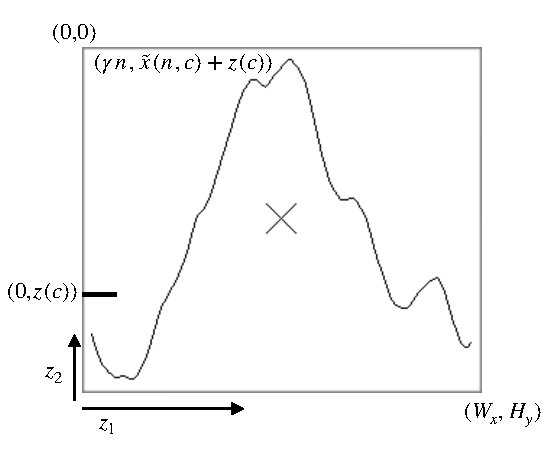
\includegraphics[scale=1.2]{images/imagecoordinatesystem.pdf}
\caption[Image Coordinate System]{The image coordinate system and the mapping from the signal segment.  The origin is the $(0,0)$ position at the upper-left corner of the image.  Time is represented as sample points on the horizontal axis, and the amplitude in $\mu V$ is shown on the vertical axis. Image height $H_y$ and width $W_x$ are obtained based on signal parameters.  The signal's zero-level $z(c)$ is the vertical location where the signal zero value is located. The plot of the signal is obtained by first setting the sample points on the predetermined image locations according to equation \ref{eq:images} and then applying a discrete interpolation algorithm to connect them with straight lines. }
\label{fig:imagecoordinatesystem}
\end{figure}

%\begin{figure}[]
%\centering
%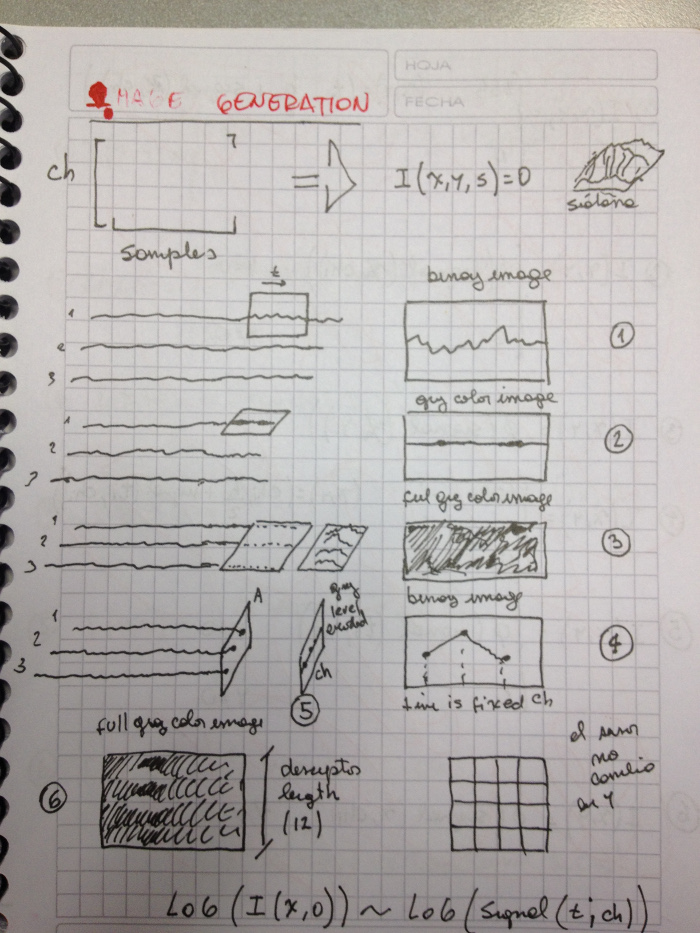
\includegraphics[scale=0.2]{images/SignalTransformation.jpg}
%\caption[EEG Signal Mapping to Images]{Six ways of mapping an EEG signal segment into a binary or greyscale image.}
%\label{fig:mappingimages}
%\end{figure}


In order to convert the EEG original signal $x(n,c)$ into an image $I(z_1,z_2)$, the following six alternatives can be used.

\begin{enumerate}
\item Channel-by-channel binary image

The standard plotting, on a black-and-white image with lines representing voltage amplitude.

\begin{equation}
I^{(c)}(z_1,z_2)= \left\{ \begin{array}{rl}
255 & \text{if} \,  z_1 =  n; \; z_2 = x(n,c) + z(c) \\
0   & \mbox{otherwise}
\end{array}\right.
\label{eq:images}
\end{equation}

\item Channel-by-channel greyscale image

The voltage amplitudes are represented in greyscale, that could range between 0 and 255.  The function $\phi( \cdot )$ is a bounded linear mapping.

\begin{equation}
I^{(c)}(z_1,z_2)= \left\{ \begin{array}{rl}
\phi(x(n,c)) & \text{if} \,  z_1 = n; \; z_2 = z(c) \\
0   & \mbox{otherwise}
\end{array}\right.
\label{eq:images}
\end{equation}

\item Multichannel full greyscale image

The image is greyscale. Voltage amplitudes are represented by the pixel content and each channel is represented on the vertical axis.  The height of the signal is equal to the number of channels.   This is used in Neuroimaging plots of ERP events.

\begin{equation}
I(z_1,z_2) = \left\{ \begin{array}{rl} \phi(x(n,c))  & \text{if} \,  z_1 = n; \; z_2 = c \end{array}\right.
\label{eq:images}
\end{equation}


\item Multichannel stationary binary image

The horizontal axis of the image is not time, but it is channels instead.   In this representation different contributions from different channels can be explored at the same time, but time dynamics is lost.  

\begin{equation}
I^{(n)}(z_1,z_2) = \left\{ \begin{array}{rl}
255 & \text{if} \,  z_1 = c; \; z_2 =  x(n,c) + z(n) \\
0   & \mbox{otherwise}
\end{array}\right.
\label{eq:images}
\end{equation}

\item Multichannel stationary greyscale image

This is a variant of the previous one, where the horizontal axis represent the channel.   In this form, the intensity of the contribution of each channel is represented by the greyscale pixel value.  Combined with head models and forward projection solutions this is the methodology used to represent scalp heatmaps~\cite{Gramfort2013}.

\begin{equation}
I^{(n)}(z_1,z_2)= \left\{ \begin{array}{rl}
\phi(x(n,c)) & \text{if} \,  z_1 = c; \; z_2 =  z(n) \\
0   & \mbox{otherwise}
\end{array}\right.
\label{eq:images}
\end{equation}


\item Channel by channel full greyscale image

This is similar to a raster plot but the greyscale image representing voltages in pixel intensities is repeated $H$ times, the height of the image.  The selection of this value is arbitrary.

\begin{equation}
I^{(c)}(z_1,z_2) = \left\{ \begin{array}{rl} \phi(x(n,c_i))  & \text{if} \,  z_1 = n; \; z_2 = H \end{array}\right.
\label{eq:images}
\end{equation}

%This last representation has the important property that $ LoG(I(x,0)) = LoG(x(n,c)) $.

\end{enumerate}

\section{EEG Signal Plot}

A binary image plot $I^{(c)}$ can be constructed according to

\begin{equation}
I^{(c)}(z_1,z_2) = \left\{ \begin{array}{rl}
255 & \text{if} \,  z_1 = \gamma_{t} \  n; \! z_2 = \left\lfloor \gamma \; \tilde{x}(n,c) \right\rceil + z(c) \\
0   & \mbox{otherwise}
\end{array}\right.
\label{eq:images}
\end{equation}

\noindent with $255$ being white and representing the signal's voltage in relation to the zero-level $z(c)$, and $0$ for black which is the background contrast. This scheme produces a black-and-white plot of the signal.  Pixel arguments $ (z_1,z_2) \in \mathbb{N} \times \mathbb{N}$ iterate over the width and height of the image plot with $1 \leq n \leq N$ and $1 \leq c \leq C$.  There is one image per channel.  The parameters $\gamma$ and $\gamma_t$ are the amplitude and time scaling factors.  They are used to determine the image size and at the same time the image resolution.

To analyze effectively an EEG signal, many signal segments must be produced.  Hence, the transformation from signal to image is continuously repeated, and many images need to be crafted for the EEG signal under analysis.  How to determine the size of all the images so that they can be effectively compared between them ?  The first option is to regularize the signal and fit in an equal size for every image.  An alternative choice is to autoscale every image according to the zero-level position.  Figure \ref{fig:plottingscheme} shows two sample artificial impulse signals and their  alternative transformation into images.

\subsection{Standardized plotting}
\label{standardized}

The \textit{z-score} is a widely used method to regularize a signal~\cite{Zhang2013}.

This standardization procedure is defined for  $1 \leq n \leq N$ and $1 \leq c \leq C$ by doing

\begin{equation}
\tilde{x}(n,c) =  \frac{( x(n,c) - \bar{x}(c)  )}{ \hat{\sigma}(c) } 
\label{eq:standarizedaverages}
\end{equation}

\noindent  where $ x(n,c) $ is the multichannel EEG signal segment for the sample point $n$ and for channel $c$. The values $$\bar{x}(c) =\frac{1}{N}\sum_{n=1}^{N}x(n,c)$$ and $$ \hat{\sigma}(c) = (\frac{1}{N-1}\sum_{n=1}^{N}(x(n,c)-\bar{x}(c))^2 )^{\frac{1}{2}}$$ are the mean and estimated standard deviation of $x(n,c), 1 \leq n \leq N$, for each channel $c$. Figure~\ref{fig:plottingscheme}(a) shows an impulse signal and their standardized representation.

\subsection{Autoscaled plotting}
\label{autoscaled}

This plotting scheme allows each image to adapt to the underlying signal.  The height is set at twice the value of the zero-level, and the signal mean is subtracted from the signal, producing a vertical displacement.

\begin{equation}
\tilde{x}(n,c) =  x(n,c) - \bar{x}(c) 
\label{eq:autoscaled}
\end{equation}

Figure \ref{fig:plottingscheme}(b) shows the results of the plotting for an impulse signal.  Equation~\ref{eq:autoscaled} has the advantage that any low frequency component, particularly the EEG DC drift is eliminated, due to the fact that plot of the signal is always centered on each image.

\begin{figure}[htb]
\centering
\subfigure[An artificial signal pulse and their plotting representation. The signal is standardized and the height of the image is determined according to the peak-to-peak amplitude, which is constant for every image and equal to $\gamma$. ]
{
\includegraphics[height=5cm,width=15cm]{images/signalplot1.eps}}
\subfigure[The plotted image height is twice the zero-level. In this case, the height is also determined according to the peak-to-peak amplitude of each segment, proportional to $\gamma$, and not constant. Transformed images do not have the same height, but the zero-level is always located at half the height of the image.]{
\includegraphics[height=5cm,width=15cm]{images/signalplot2.eps}}
\caption[Signal plot of an impulse response]{Signal plotting schemes.}
\label{fig:plottingscheme}
\end{figure}

\subsection{Zero-Level}

The zero-level $z(c)$ is the image vertical position where the signal's zero value has to be situated in order to fit the entire signal within the image for each channel c:

\begin{equation}
z(c) = \left \lfloor{ \frac{\max_{n} \tilde{x}(n,c)  - \min_{n} \tilde{x}(n,c) }{2} }\right \rfloor -   \left \lfloor{ \frac{\max_{n} \tilde{x}(n,c)  + \min_{n} \tilde{x}(n,c)}{ 2} }\right \rfloor
\label{eq:zerolevel}
\end{equation}

\noindent where the minimization and maximization are carried out for $n$ varying between ${1 \leq n\leq N}$, and $ \lfloor \cdot  \rfloor $ denote the rounding to the smaller nearest integer of the number.  This value represents the vertical location on the image where the signal goes to zero.  

\subsection{Image Size}

\subsubsection{Height}

The height of the image is calculated according to the peak-to-peak amplitude of the signal,

\begin{equation}
H_y = \max \left\lfloor \gamma \; \tilde{x}(n,c) \right\rceil  - \min \left\lfloor \gamma \; \tilde{x}(n,c) \right\rceil 
\label{eq:height}
\end{equation}

\noindent while for the autoscalable version, it is just twice the value of the zero-level.

\begin{equation}
H_y = 2 \; z(c)
\label{eq:autoscaleheight}
\end{equation}


\subsubsection{Width}

The width on the other hand is obtained based on the length of the signal segment, scaled by the $\gamma_t$  time factor,

\begin{equation}
W_x = \gamma_t  N
\label{eq:width}
\end{equation}


\subsection{Interpolation}

Equation \ref{eq:images} produces a set of isolated pixels over the image.  To produce the plot $I^{(c)}$, the Bresenham \cite{Bresenham1965,Ramele2016} algorithm is used to digitally interpolate straight lines between each pair of consecutive pixels.  Figure~\ref{fig:interpolation}(a) shows an image plot constructed by only using the sample points, while (b) shows the digital interpolation produced by the Bresenham algorithm.

\begin{figure}[h!]
\centering
\subfigure[Sample points are located on the image according to Equation \ref{eq:images}. ]
{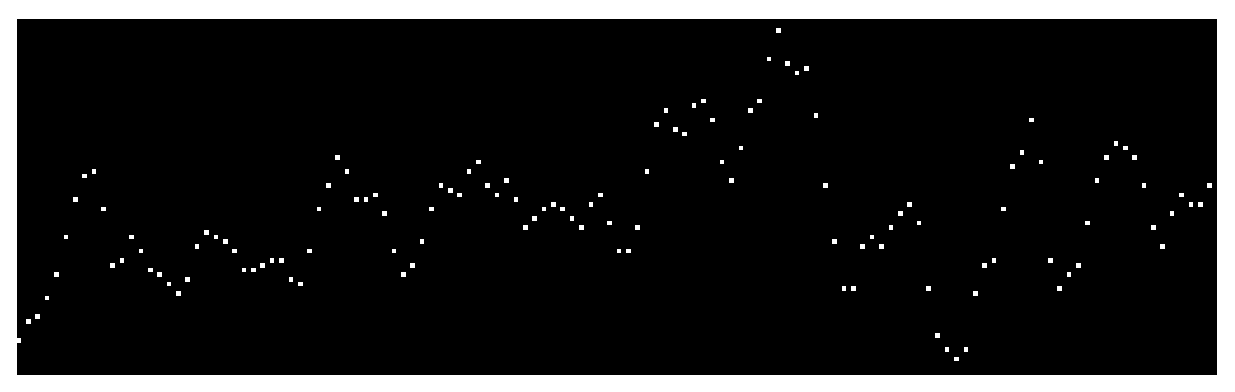
\includegraphics[height=4cm,width=15cm]{images/samplepoints.eps}}
\subfigure[Sample points are linearly interpolated in a discrete procedure using the Bresenham algorithm.]
{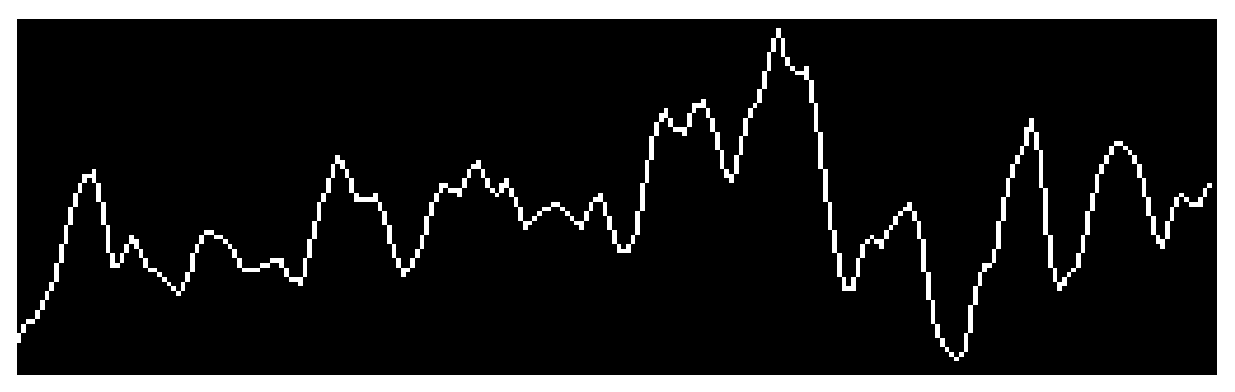
\includegraphics[height=4cm,width=15cm]{images/bresenham.eps}}
\subfigure[The digital signal is scaled 4 times ($\gamma_t=4$) and the generated sample points are interpolated using the Bresenham algorithm.]
{
\includegraphics[height=4cm,width=15cm]{images/upscaled.eps}}
\subfigure[The digital signal is upsampled 4 times and the generated sample points are interpolated using the Bresenham algorithm.]
{
\includegraphics[height=4cm,width=15cm]{images/upsample.eps}}
\caption[Signal Plotting: Interpolation]{Generated images based on different interpolation schemes.}
\label{fig:interpolation}
\end{figure}

On Figure~\ref{fig:interpolation}(c) the same signal can be observed produced when the time scaling factor $\gls{gammat}$ is increased to $4$. It can be observer that there are very sharp edges around sample pixels.  This can lead to a quantization of histogram gradients that will be discussed in the next Chapter. To reduce this sharpness of the signal on the plot, an alternative is to use a smoothing interpolation of the signal $\tilde{x}(n,c)$ using splines.  Instead of just situating time point values at a bigger step according to Equation~\ref{eq:images}, intermediate values are produced according to a linear quadratic or cubic interpolation, which smooths the curve around each point.  This procedure is similar to what the Matlab's \textbf{resample} function does which also includes an antialiasing FIR lowpass filter.

Special care must be taken by the presence of artifacts around the signal endpoints, at the edges of the image. Those regions are excluded from further analysis.

\subsection{Resolution and Precision}

The resolution~\cite{Cohen2014} of the image transformation can be determined based on the characteristics of the digital signal and the parameter selection.

On the horizontal axis of the image, one pixel is equivalent to 

\begin{equation}
1 P_x \equiv \frac{1}{F_s  \; \gamma_t}  [\si{s}]
\label{eq:resolutionx}
\end{equation}

\noindent where $F_s$ is the sampling frequency in Hertz, and $\gamma_t$ is the time scale factor.  This gives a value in seconds.  For example, for Figure \ref{fig:imagecoordinatesystem}, the sampling frequency is $200 Hz$, the length is $0.65 s$ and $\gamma_t = 1$, which gives a resolution of $1 P_x \equiv 0.0077 s$. 

Consistently, on the vertical axis, one pixel is analogous to 

\begin{equation}
1 P_y \equiv \frac{1}{\gamma}  [\si\mu{V}]
\label{eq:resolutiony}
\end{equation}

\noindent where $\gamma$ is the amplitude scale factor.  As EEG time-series are digitalized in $\si\mu{V}$, this the unit of choice.  In Figure \ref{fig:imagecoordinatesystem}, $1$ vertical pixel represents exactly $1 \mu V$.

Regarding the \textit{Precision}, EEG time-series are floating-point numbers and the image is constructed based on discrete and integer pixels.  Image's pixel values $(z_1,z_2)$ are obtained according to Equation~\ref{eq:images}.  Thus, on the horizontal axis, $z_1$, no discretization is needed because time is already digitalized in sample units. Hence, there is no loss of precision in time from the one generated by the digital device.

\begin{equation}
z_1 = \gamma_t  \; n.
\label{eq:horizontalpixelation}
\end{equation}

On the other hand, on the vertical axis, pixels are discretized according to

\begin{equation}
z_2 = \left \lfloor{ \gamma  \; \tilde{x}(n,c)  }\right \rceil
\label{eq:verticalpixelation}
\end{equation}

\noindent where $\gamma$ is the scale amplitude factor parameter, which also affects the height of the image in Equation \ref{eq:height}. A rounding operation $\lfloor  \cdot \rceil$ is applied to obtain an integer value.  Hence, precision is lost on the voltage amplitude. Additionally, the dynamic range of the digital capturing device is reduced to what is actually needed for each segment.  Table~\ref{tab:precision} show some reference values.

\begin{table}[htb]
\caption[Reference Values for Precision and Resolution]{Reference Values for Precision and Resolution}
\centering
%% \tablesize{} %% You can specify the fontsize here, e.g.  \tablesize{\footnotesize}. If commented out \small will be used.
\begin{tabular}{c|c|c||c|c|c}
\toprule
\textbf{$\gamma$}	&  $1 P_x$ 	&  Decimal Precision & \textbf{$\gamma_t$}	&  $1 P_y$  \\
\midrule
1     &     $1 \si\mu{V}$   &  $NN$                               & 1    &     $\frac{1}{\gls{Fs}} \si{s}$    \\
2    &     $\frac{1}{2} \si\mu{V}$   &  $NN \pm 0.5$  & 2    &     $\frac{1}{2} \; \frac{1}{\gls{Fs}} \si{s}$    \\
3     &     $\frac{1}{3} \si\mu{V}$   &  $NN\pm 0.3$  & 3    &     $\frac{1}{3} \;  \frac{1}{\gls{Fs}} \si{s}$    \\
10     &     $\frac{1}{10} \si\mu{V}$   &  $NN.N$        & 10   &     $\frac{1}{10} \; \frac{1}{\gls{Fs}} \si{s}$    \\
100     &     $\frac{1}{100} \si\mu{V}$   &  $NN.NN$ & 100 &     $\frac{1}{100} \; \frac{1}{\gls{Fs}} \si{s}$    \\
\bottomrule
\end{tabular}
\label{tab:precision}
\end{table}

\chapter{The Histogram of Gradient Orientations of Signal Plots}
\label{chapter:three}

This Chapter presents and introduce the EEG feature extraction procedure based on the Histogram of Gradient Orientations.  This method is grounded on an extension and modification of the SIFT~\cite{Lowe2004} Descriptor which is used in Computer Vision to extract and map local regions of an image.  At the same time, this Chapter fill in and end the previous Chapter, describing how to mine the information from the Plot and build a feature out of it.

\section{Introduction}

%sinuplot, spectrogram, scalogram

The work of Edelman, Intrator and Poggio~\cite{cogprints561} on how the visual cortex sense features was the inspiration to the development of an algorithm to identify and decode salient local information from image regions.  SIFT is composed of two parts, the SIFT Detector and the SIFT Descriptor.  The first one is the procedure to identify relevant areas of an image.  The second one is the procedure to describe and characterize a region of an image using the Histogram of Gradient Orientations~\footnote{It should not to be confused with HOG~\cite{Dalal2005}, the Histogram Of Gradients which is another method from Computer Vision based on similar ideas.  Actually, the descriptor part of the SIFT Method has no specific name, but as it is based on building a histogram of gradient orientations, that is the reason why it is described here in that way. }.  The SIFT algorithm is biomimetically inspired in how the visual cortex detects shapes by analyzing orientations~\cite{cogprints561}.  The patch description is also based on the Theory of Receptive Fields and other related ideas~\cite{Lindeberg2013}.

\section{Feature Extraction: Histogram of Gradient Orientations}
\label{SIFT}

On the image generated by the procedure detailed in previous Chapter, a keypoint $\gls{kp}$ is placed on a pixel $(x_{kp}, y_{kp})$ over the image plot and a window around the keypoint is considered. A local image patch of size $\gls{Sx} \times \gls{Sy}$ pixels is constructed by dividing the window in $16$ blocks. It is arranged in a $4 \times 4$ grid and the pixel $\gls{kp}$ is the patch center. 

A local representation of the signal shape within the patch can be described by obtaining the gradient orientations on each of the $16$ blocks and creating a histogram of gradients.  This technique is the basis of Lowe's SIFT Descriptor method. In order to calculate the histogram, the interval $[0-360]$ of possible angles is divided in $8$ bins, each one at $45$ degrees.

 Hence, for each spacial bin $ i,j = \{0,1,2,3\} $, corresponding to the indexes of each block $B_{i,j}$,  the orientations are accumulated in a  $3$-dimensional histogram $h$ through the following equation: 
 

\begin{equation}
 h(\theta,i,j) = \sum_{\mathbf{p}} w_\mathrm{ang}(\angle J(\mathbf{p}) - \theta)\, w_{ij}\left(\mathbf{p} - \mathbf{kp} \right)\, |J(\mathbf{p})|
\label{eq:histogram}
\end{equation}

\noindent  where $\mathbf{p}$ is a pixel from within the patch,  $\theta$ is the angle bin with $ \theta \in \{0, 45, 90, 135, 180, 225, 270, 315\} $,  $ |J(\mathbf{p})| $ is the norm of the gradient vector in the pixel $\mathbf{p}$ and it is computed using finite differences and $\angle J(\mathbf{p}) $ is the angle of the gradient vector.  The scalar $ w_\mathrm{ang}(\cdot) $  and vector $ w_{ij}(\cdot) $ functions are linear interpolations used by~\cite{Lowe2004} and \cite{Vedaldi2010} to provide a weighting contribution to eight adjacent bins.  They are calculated as  

\begin{equation}
 w_{ij}(\mathbf{v}) = w( \frac{v_x - x_i}{3 \; \gls{Sx}} ) w( \frac{v_y - y_i}{3 \; \gls{Sy}} ) 
\label{eq:ij}
\end{equation}

\begin{equation}
 w_\mathrm{ang}(\alpha) = \sum_{k} w( \frac{8\alpha}{2\pi} + 8r)
\label{eq:wang}
\end{equation}

\noindent where $x_i$ and $y_i$ are the spatial bin centers located in $ x_i,y_i = \{-\frac{3}{2},-\frac{1}{2},\frac{1}{2},\frac{3}{2}\} $. The function parameter $\mathbf{v} = ( v_x, v_y ) $ is a vector variable and $\alpha$ a scalar variable.  On the other hand, $r$ is an integer that can vary freely which allows the argument $\alpha$ to be unconstrained in terms of its values in radians. The interpolating function $w(\cdot)$ is defined as:

\begin{equation}
 w(z) = \max(0,|z|-1).
\label{eq:weighting}
\end{equation}

These binning functions conform a trilinear interpolation that has a combined effect of sharing the contribution of each oriented gradient between their eight adjacent bins in a tridimensional cube in the histogram space, and zero everywhere else.

Lastly, the fixed value of $ 3 $ is a magnification factor, a fixed parameter.  As the patch has  $16$ blocks and  $8$ bin angles are considered, a feature called \textit{descriptor} of $128$ dimension is obtained. 
%It can be observed that the histogram is computed by multiplying by $ |J(\mathbf{p})| $, so the method considers both, the magnitude and the orientation of the gradient vector. 

Figure~\ref{fig:sampledescriptor} shows an example of a patch and a scheme of the histogram computation. In (A) a plot of the signal and the patch centered around the keypoint is shown. In (B) the possible orientations on each patch are illustrated.  Only the upper-left four blocks are visible.  The first eight orientations of the first block, are labeled from $1$ to $8$ clockwise. The orientations of the second block $ B_{1,2} $ are labeled from $9$ to $16$.  This labeling continues left-to-right, up-down until the eight orientations for all the sixteen blocks are assigned. They form the corresponding $\mathbf{kp}$-descriptor of $128$ coordinates. Finally, in (C) an enlarged image plot is shown where the oriented gradient vector for each pixel can be seen.

\begin{figure}[h!]
\centering
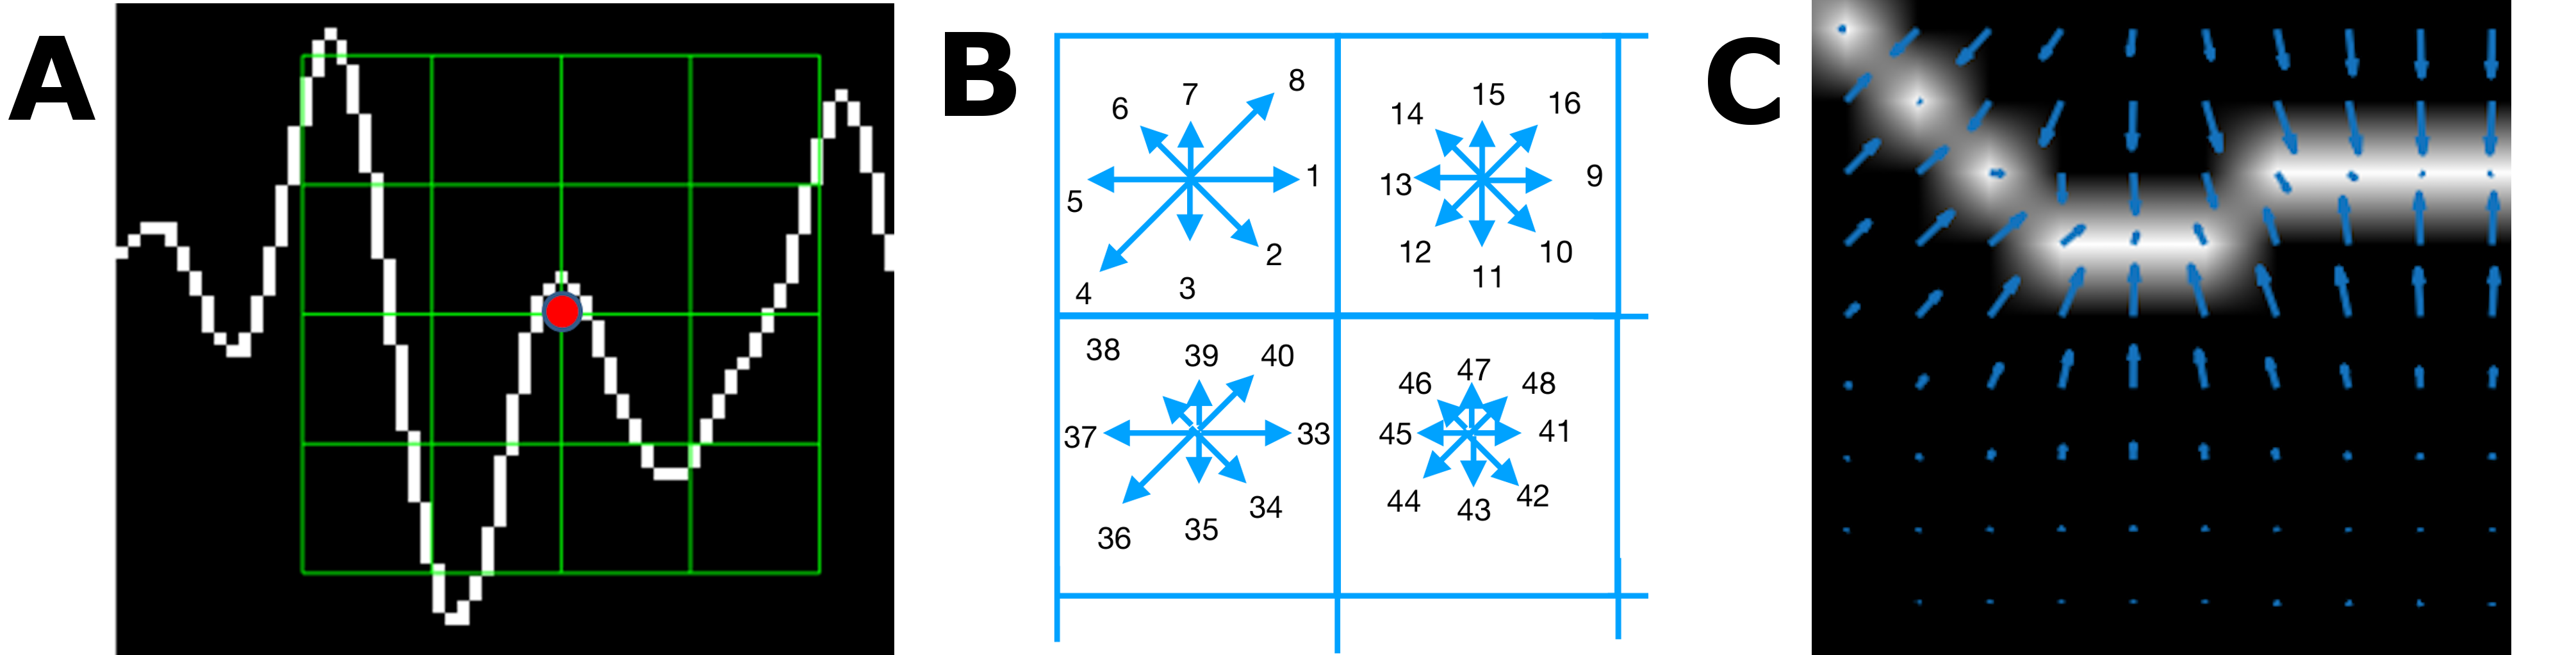
\includegraphics[width=16cm]{images/gradients.png}\label{samplegradients}
\caption[Histogram of Gradient Orientations for ERP]{ (A) Example of a plot of the signal, a keypoint and the corresponding patch. (B) A scheme of the orientation's histogram computation.  Only the upper-left four blocks are visible.  The first eight orientations of the first block, are labeled from $1$ to $8$ clockwise. The orientation of the second block $ B_{1,2} $ is labeled from $9$ to $16$.  This labeling continues left-to-right, up-down until the eight orientations for all the sixteen blocks are assigned. They form the corresponding descriptor of $128$ coordinates.  The length of each arrow represent the value of the histogram on each direction for each block. (C) Vector field of oriented gradients.  Each pixel is assigned an orientation and magnitude calculated  using finite differences. }
\label{fig:sampledescriptor}
\end{figure}

%\begin{figure}[h!]
%\centering
%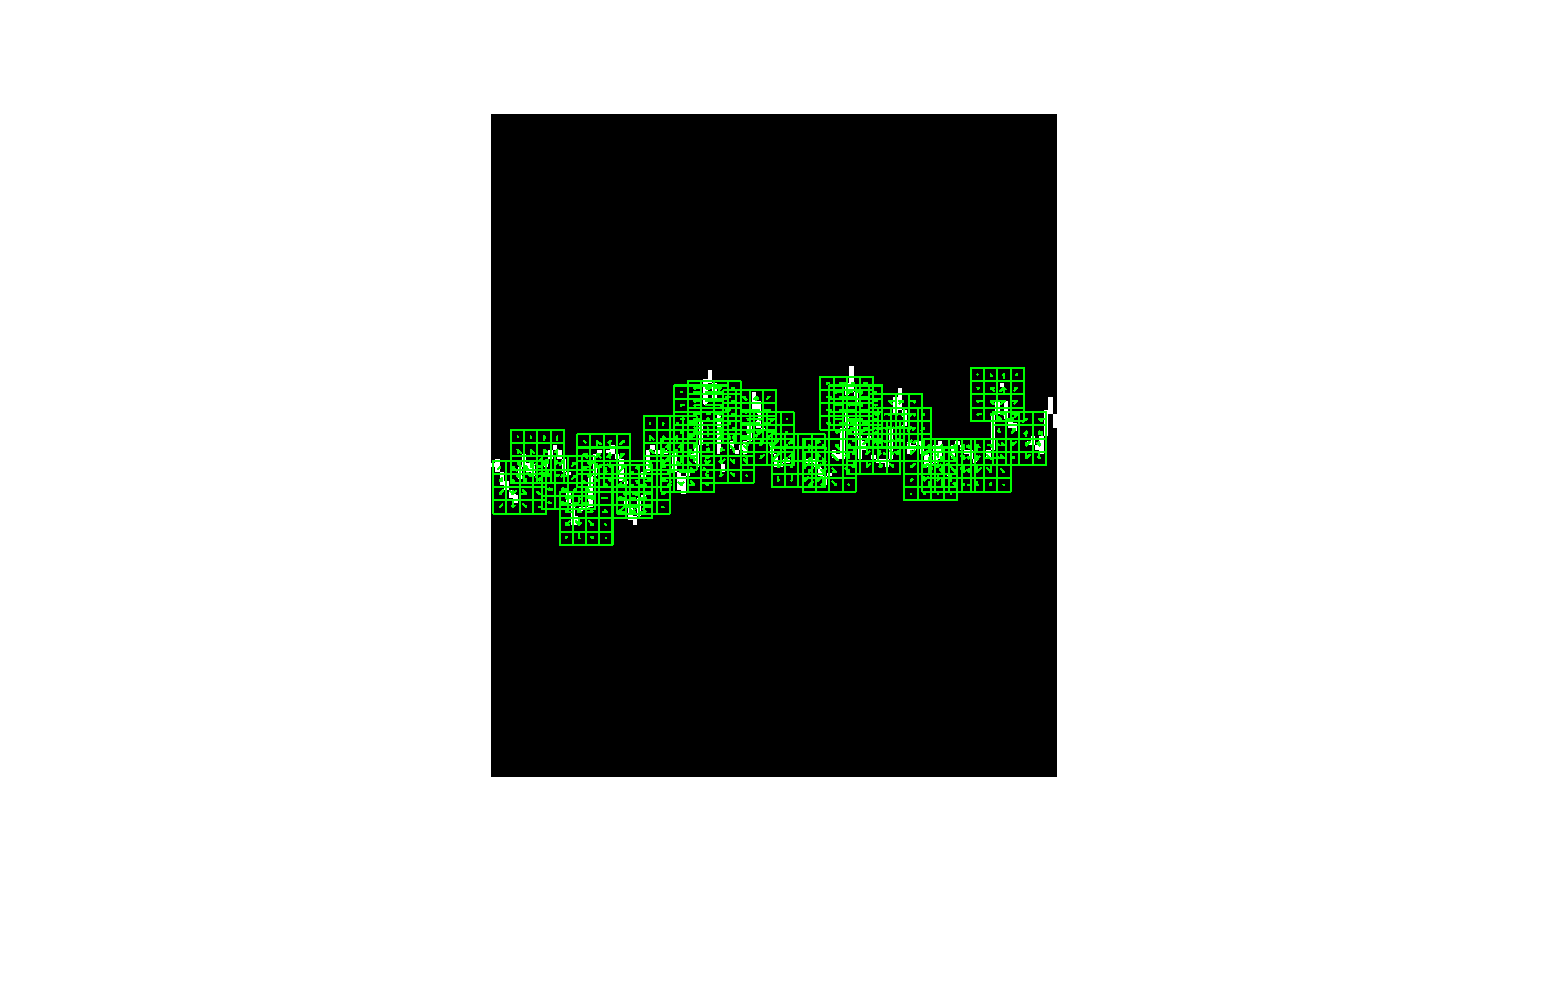
\includegraphics[scale=0.6]{images/KeypointLocations.eps}
%\caption[SIFT Patches]{fdsfdfsfs }
%\label{fig:siftpatch}
%\end{figure}


\section{Keypoint Location}

%TODO Vertidal: Along the signal or zero level.
% Horizontal: based on a cognitive event, one or many.
%



The keypoint $\gls{kp}$ location must be accurate specified in order to establish the region from the signal where the waveform is located.

For the horizontal position, the localization of the keypoint is based on a priori information, based on the characteristics of the event under study.  For instance certain ERP have a specific timing that can be explored to elucidate in which position the expected signal pattern will be generated.

But the main answer to respond is how many descriptors, and this also leads to density of descriptors.  How many per pixel or per sample point.

Additionally, there can be more than just one patch located over the signal plot.  This is particular important for oscillatory processes and defines a descriptor density parameter $s_d$.

\begin{figure}[h!]
\centering
\subfigure[]
{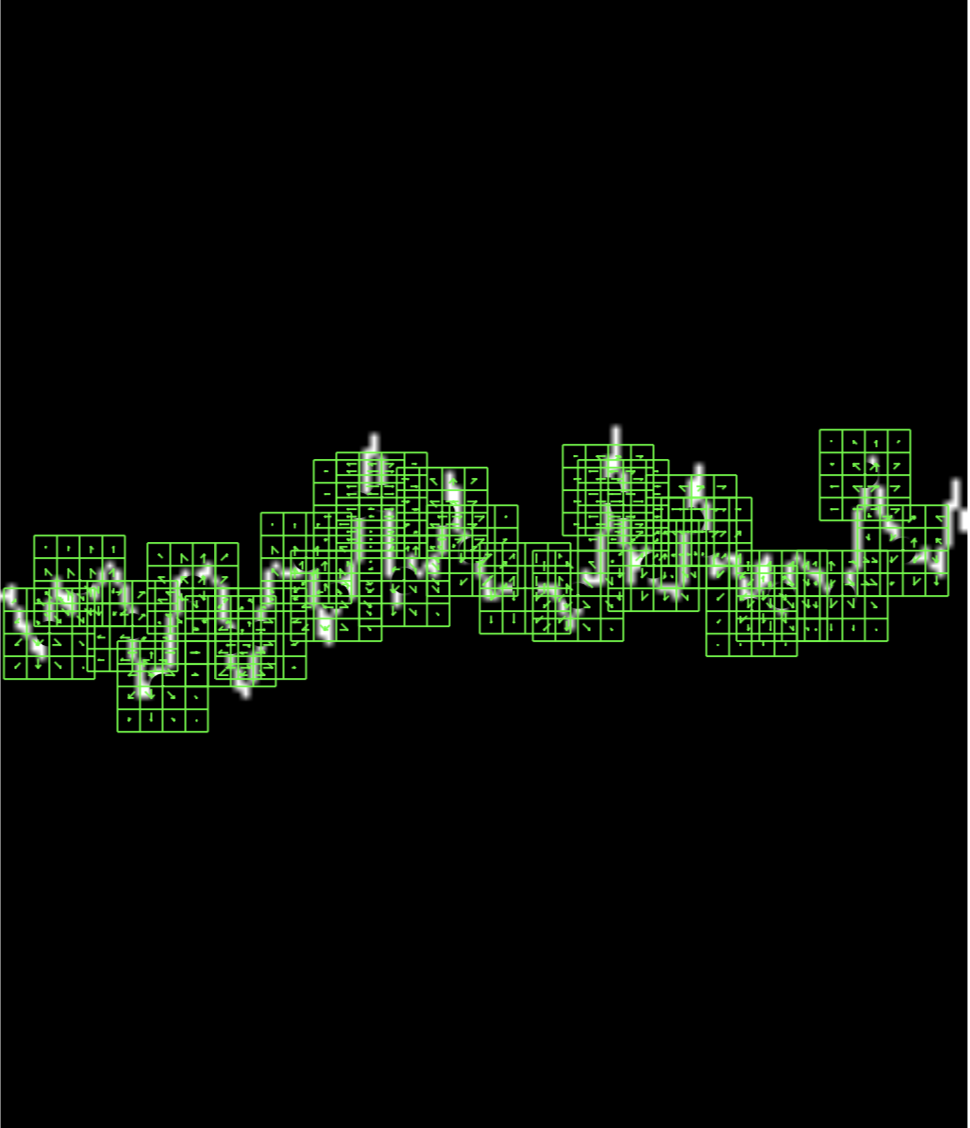
\includegraphics[width=6cm, height=6cm]{images/SignalWithFullDescriptors3.png}}
\subfigure[]
{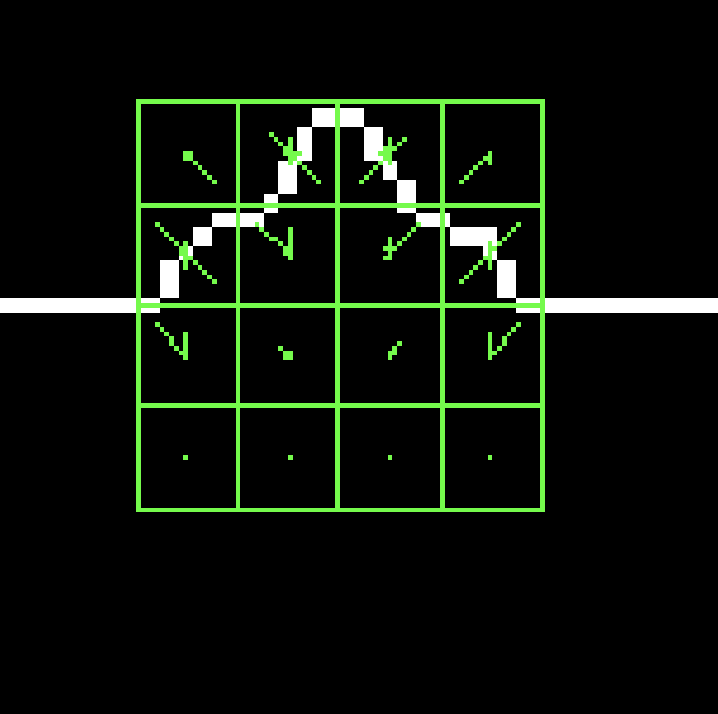
\includegraphics[width=6cm, height=6cm]{images/EasyDescriptorSample3.png}}
\subfigure[]
{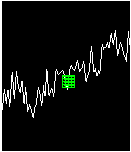
\includegraphics[width=6cm, height=6cm]{images/SignalWithDescriptorSample1.png}}
\subfigure[]
{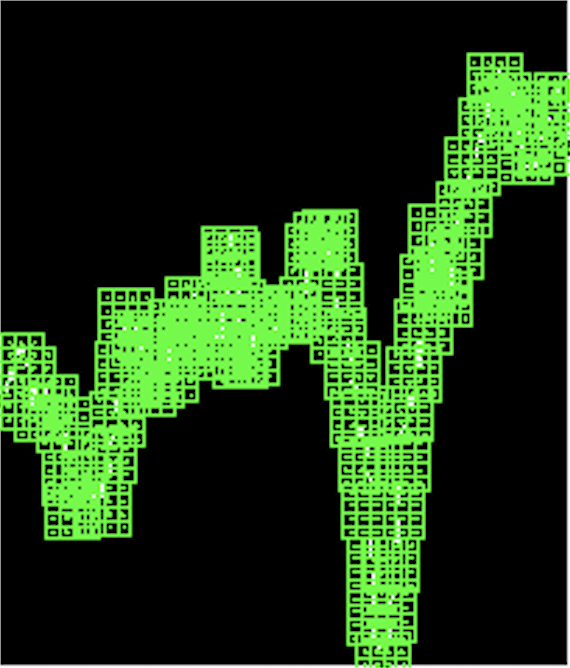
\includegraphics[width=6cm, height=6cm]{images/SignalWithFullDescriptors2.png}}
\caption[Keypoint Locations]{}.
\label{fig:keypointlocations}
\end{figure}

Regarding the Vertical Location, there are two options.  The first one is along the signal, exactly on the sample points calculated by the Equation \ref{eq:images}.  The second is on a fixed position over the zero-level as described by \ref{eq:zerolevel}.

\section{Patch Geometry}

%TODO Vertical size: Fixed for autoscaled and variable.
% Horizontal: based on a priori information


The Horizontal Patch Scale $\gls{St}$ determines the size of the patch on the image horizontal axis, and it is related to the span $\gls{lambda}$ of the waveform to analyze according to

\begin{equation}
\gls{St} = \frac{ \gls{lambda} \;  \  \gls{Fs} \ \gls{gammat} }{\gls{Deltas}}
\label{eq:horizontalpatchscale}
\end{equation}

\noindent where $\gls{Fs}$ is the sample frequency, $\gls{gammat}$ is the time scale factor and $\gls{Deltas}$ is the pixel conversion factor.

On the other hand, on the vertical axis, the vertical patch scale depends on the peak-to-peak amplitude $\gls{DeltamuV}$.

\begin{equation}
\gls{Sv} = \frac{\gls{St} \ \gls{gamma}}{\gls{Deltas}} 
\label{eq:mapping1}
\end{equation}

The vertical scale can be dynamically adjusted according to the peak-to-peak amplitude of each segment, or it can be set fixed.  This is more appropiate if the underlying signal is bounded which is the case if the standardized procedure described in \ref{standardized} is applied.

Figure~\ref{fig:patchgeometry} shows the different parameters of the patch.

\begin{figure}[h!]
\centering
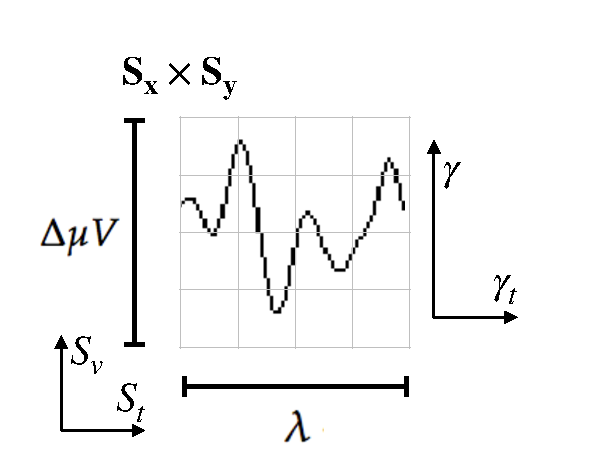
\includegraphics[width=10cm]{images/patchgeometry.pdf}
\caption[Patch Geometry]{The scale of local patch is selected in order to capture the whole transient event.  The size of the patch is $\gls{Sy} \times \gls{Sx}$ pixels. The vertical size consists of $4$ blocks of size $\gls{Sy}$ pixels which should be high enough as to contain the signal $\gls{DeltamuV}$, the peak-to-peak amplitude of the signal component. The horizontal size includes $4$ blocks up to $\gls{Sx}$ and should covert the entire duration in seconds of the signal waveform, $ \gls{lambda} $.   }
\label{fig:patchgeometry}
\end{figure}

Once this parameters are set, the size in pixels of the patch can be obtained in both dimensions.  The Horizontal Patch Size in pixels is

\begin{equation}
\gls{Sx} = \gls{Deltas} \; \gls{St} + 1.
\label{eq:sx}
\end{equation}

The Vertical Patch Size in pixels can be calculated from

\begin{equation}
\gls{Sy} = \gls{Deltas} \; \gls{Sv} + 1
\label{eq:sy}
\end{equation}

\noindent where $\gls{Deltas}$ is a fixed parameter value which depends on the SIFT implementation. The parameters $\gls{St}$  and $\gls{Sv}$ are the scales of the local patch. This region is arranged in a $4 \times 4$ grid and the pixel $\gls{kp}$ is the patch center. 

The patch size cannot be bigger than the image.  This is reflected by the following two inequalities that restrict the size of the patch according to 

\begin{equation}
\frac{\gls{Wx}-1}{\gls{Deltas}}  \geq \gls{St} 
\label{eq:restriction1}
\end{equation}

\noindent on the horizontal axis, and on the vertical axis, 

\begin{equation}
\frac{\gls{Hy}-1}{\gls{Deltas}}  \geq \gls{Sv}.
\label{eq:restriction2}
\end{equation}

\subsection{Oscillatory Processes}

For these patterns, the central idea is to locate keypoints, and their patches and descriptors, all along the signal trace and filling the entire signal segments with all the possible descriptors.  In this case, the descriptor density determines the step at which a keypoint is located along the trace of the signal, pixel after pixel.  Close to the margins, there is a gap to avoid locating incomplete patches.  This can be observed in Figure~\ref{fig:keypointlocations}(a).

\subsection{Transient Events}

For transient events, descriptors are treated as representatives of the signals itself so there is just one descriptor that is located in a meaningfull position along the time axis.

Additionally, particularly for autoscale plotting, the zero level can be used to localize keypoints.

\section{Classification}
\label{nbnn}

A discriminative~\cite{WolpawJonathanR2012} semi-supervised classification method based on Naive Bayes Nearest Neighbor~\cite{Boiman2008} was applied to classify EEG signals using the features provided by the calculated descriptors.
One problem that frequently arises when using local features is how to go back from the classification of those local characteristics to the image where those descriptors came from.
The NBNN technique overcomes this problem by comparing each image against a whole class which is characterized by the set of descriptors that are closest to each one of the descriptors of the query image. This algorithm is very easy to implement, and is based on (5).

\begin{equation}
\hat{class} = \arg \min_{class} \sum_{\mathbf{d_i}^{(c)}} \sum_{q \in N_T(\mathbf{d_i}^{(c)})}^{} {\left\lVert q -  \mathbf{d_i}^{(c)} \right\rVert}  ^{2}
\label{eq:multiclassificationrow}
\end{equation}

The estimated class C of a query image is calculated as the class C that minimize the summation of the L2 distance between each descriptor di that belongs to the query image and its corresponding near neighbot NNc(di) descriptor for each class.

In brief, based on segmented signals from at least two labeled classes, a set of images is first generated.  For each image, desctipros are extracted during the training or calibration step of a BCI procedure and they are grouped in KD-tree~\cite{Lowe2004} structures for each one of the classes.

Hence, given a new unlabeled signal segment, an image plot is generated as well, and their descriptors extracted.  They are fed into Equation 5 in order to determine the class which minimizes the summation and thus provide the information bit to the BCI controller.  


\begin{figure}[h!]
\centering
\subfigure[]
{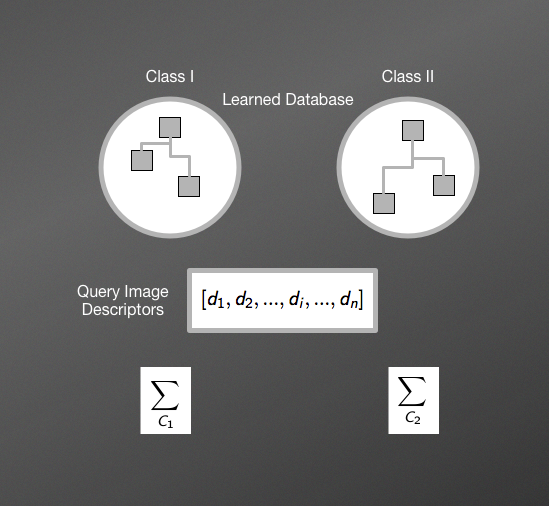
\includegraphics[scale=0.25]{images/NBNNMethod1.png}}
\subfigure[]
{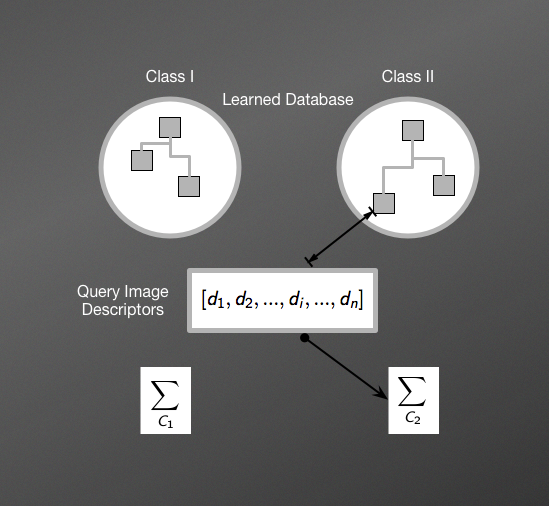
\includegraphics[scale=0.25]{images/NBNNMethod2.png}}
\subfigure[]
{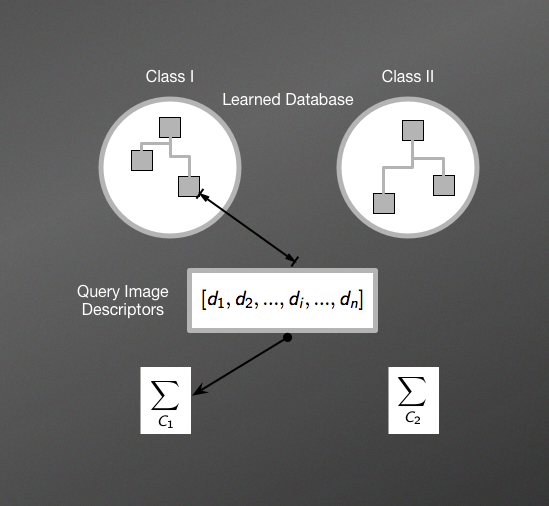
\includegraphics[scale=0.25]{images/NBNNMethod3.png}}
\subfigure[]
{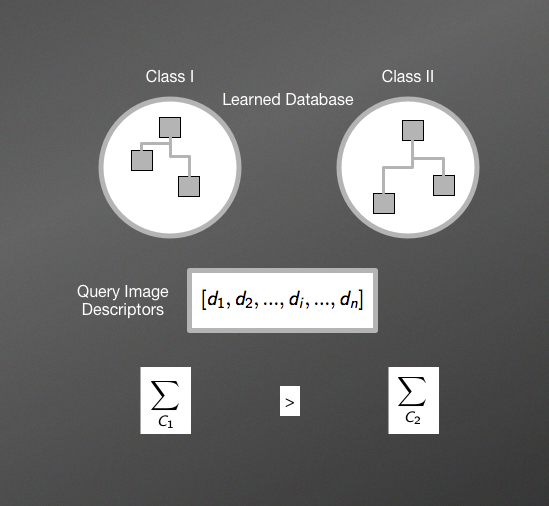
\includegraphics[scale=0.25]{images/NBNNMethod4.png}}
\subfigure[ ]
{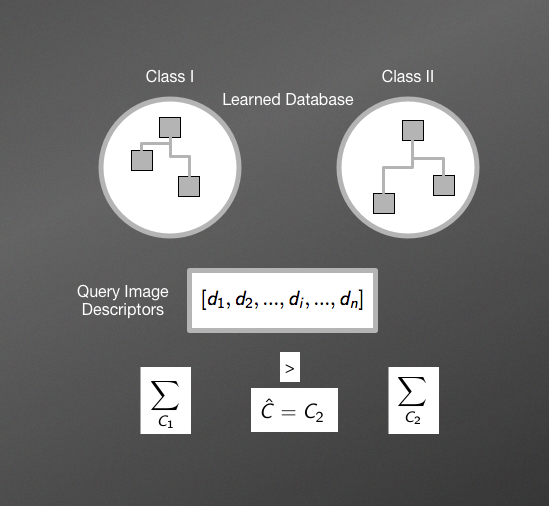
\includegraphics[scale=0.25]{images/NBNNMethod5.png}}
\caption[NBNN Classification]{(a) Two Dictionaries contain templates descriptors for two different classes. A set of query descriptors are extracted from a new image that needs to be categorized.(b) Distances from every descriptor $di$ is calculated against the closest one from the Dictionary of Class 2.  Distances are accumulated.(c) Distances from every descriptor $di$ is calculated against the closest one from the Dictionary of Class 1.  Distances are accumulated. (d) The two different values are compared.(e) The summation that achieved the lesser value is the one that more closely resemble the set of templates, thus is the one predicted by the classification algorithm.}
\label{fig:nbnnclassification}
\end{figure}

%TODO:Agregar tambien las pruebas sobre rootsift y que la distancia mejor es la coseno demostrar justamente haciendo una prueba sobre EEGWave.
%TODO:Agregar que el experimento dio perfecto cuando no se controla la varianza.

\section{BCI Algorithm}

In brief, based on segmented signals from at least two labeled classes, a set of images is first generated.  For each image, desctipros are extracted during the training or calibration step of a BCI procedure and they are grouped in KD-tree~\cite{Lowe2004} structures for each one of the classes.

Hence, given a new unlabeled signal segment, an image plot is generated as well, and their descriptors extracted.  They are fed into Equation 5 in order to determine the class which minimizes the summation and thus provide the information bit to the BCI controller.  

\section{Implementation}

\subsection{Matlab, C++ and VLFeat}

The implemented code is published in \url{https://bitbucket.org/itba/hist/} by using Matlab, python and the VLFeat library.

%TODO add the data and also the code ocean repository.  Also add my own repositories.

\section{Mapping Cheat-Sheet}

This section provides a mapping cheat sheet to convert and obtain the parameters of the algorithm for a given set of signal parameters.

The input signal parameters are $N$,$F_s$ and $\lambda$. The peak-to-peak amplitude of the waveform to study is $ \Delta \mu V $. The unit length of the patch is $\Delta_s = \sqrt{2} \; 15$.  

Output parameters are: 
$\gls{N}$, 
$\gls{lambda}$
$\gls{Fs}$
$\gls{Deltas}$
$\gls{DeltamuV}$
$\gls{gamma}$
$\gls{gammat}$
$\gls{Hy}$
$\gls{Wx}$
$\gls{St}$
$\gls{Sv}$
$\gls{Sy}$
$\gls{Sx}$
$\gls{w}$
$\gls{kp}$
$\gls{P}$

Amplitude scale factor

\begin{equation}
\gamma \equiv \frac{H_y}{\Delta \mu V}  
\label{eq:gammadefinition}
\end{equation}

Time scale factor

\begin{equation}
\gamma_t \equiv \frac{W_x}{F_s \; w}  
\label{eq:gammatdefinition}
\end{equation}

%\begin{equation}
%s_x = \frac{ \gamma \;  \lambda \  F_s}{12}
%\label{eq:mapping2}
%\end{equation}
%
%\begin{equation}
%s_y= \frac{\gamma \; \Delta \mu V}{12} 
%\label{eq:mapping1}
%\end{equation}

Restriction on the waveform time scale

\begin{equation}
\frac{W_x-1}{\sqrt{2} \; 15}  \geq S_t 
\label{eq:restriction1}
\end{equation}

Restriction on the waveform amplitude scale

\begin{equation}
\frac{H_y-1}{\sqrt{2} \; 15}  \geq S_v 
\label{eq:restriction2}
\end{equation}

Horizontal Patch scale

\begin{equation}
S_t = \frac{ \lambda \;  \  F_s \ \gamma_t }{\Delta_s}
\label{eq:mapping2}
\end{equation}

Vertical Patch scale

\begin{equation}
S_v= \frac{\Delta \mu V \ \gamma}{\Delta_s} 
\label{eq:mapping1}
\end{equation}

Time to sample point conversion

\begin{equation}
n = \left\lfloor F_s \ \Delta_t \right\rfloor \ \gamma_t
\label{eq:mapping1}
\end{equation}

Horizontal Patch size in pixels

\begin{equation}
\mathbf{S}_x = \Delta_s \; S_t + 1
\label{eq:mapping2}
\end{equation}

Vertical Patch Size in pixels

\begin{equation}
\mathbf{S}_y = \Delta_s \; S_v + 1
\label{eq:mapping1}
\end{equation}

Span of a Patch

\begin{equation}
\Delta_t = \frac{S_t \ \Delta_s}{F_s \ \gamma_t} 
\label{eq:mapping1}
\end{equation}

\chapter{Alpha Wave: inhibition signal}
\label{chapter:four}
\epigraph{The electroencephalogram represents a continuous curve with continuous oscillations in which... one can distinguish larger first order waves with an average duration of 90 milliseconds...}{Berger}

This Chapter describes the experiments performed over a well-established but still mysterious EEG cognitive signal: The Berger Rhythm or Visual Occipital Alpha Waves.  An own dataset of resting subjects while maintaining their eyes open and closed is produced and the details of their generation are outlined.  Additionally, an experiment on a public Dataset is also detailed.  Conclusions and discussion is described in the last section.

\section{Introduction}

%We gather the first dataset  using the EEG EPOC Emotiv Headset and we  access the raw signals using its C++ SDK provided by the manufacturer.  The device sends wirelessly  digitalized 128 Hz sampled EEG information as discrete packets.  Every packet is numbered and the electronic impedance is constantly measured, and delivered as part of the packet information. The wireless transmitter connects to a standard RF dongle which receives the information from  14 channels and forwards it into the PC, particularly to a custom C++ EEG Datalogger program that was developed in-house.  The program is waiting passively until a new packet is received from the dongle, verifying the packet numbering and controlling that the impedance is bellow a certain level, according to the device's documentation \cite{c11}. 

Alpha Waves were the first signals ever spotted from the Electroencephalography.  They are very well characterized as 10 Hz signals, physiologically consistent across subjects, and they are associated with synchronous inhibitory processes and attention shifting~\cite{c3}. They tend to be more prominent while subject's eyes are closed and appear stronger in occipital regions, around $O_1$ and $O_2$~\cite{c6,c11}. It is also called the Posterior Dominant Rhythm due to their pervasiveness in EEG~\cite{Schomer2010}.

Figure~\ref{fig:alphawavessignals} shows two records of 8 channels signals.  The signals in Figure ~\ref{fig:alphawavessignals}(a) contains the registered alpha waves with open eyes while the (b) contains the same information with their eyes closed.  The characteristic pattern of wiggles can be spotted in the Figure ~\ref{fig:alphawavessignals}(b).

\begin{figure}[h!]
\centering
\subfigure[EEG signals of a relaxed healthy subject with their eyes open.]
{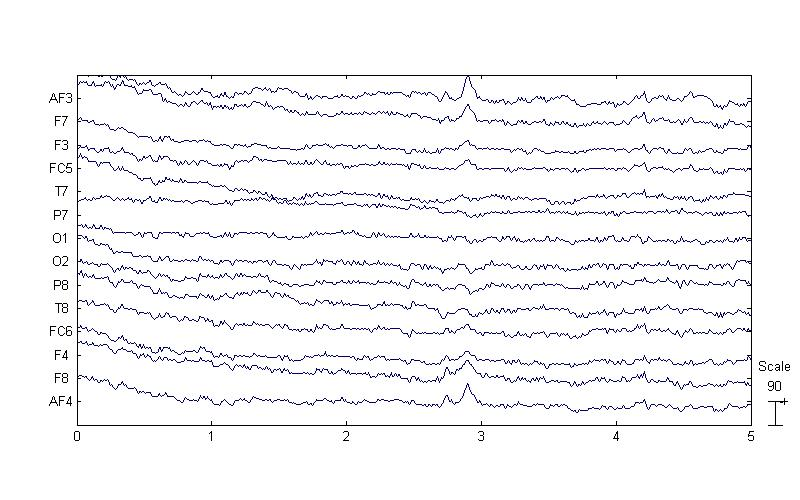
\includegraphics[height=5cm,width=7.5cm]{images/eeglab1.jpg}}
\subfigure[EEG signals of the same relaxed subject sit in front of the Computer Monitor with his eyes closed. Alpha Waves wiggles can be spotted since the first second.]
{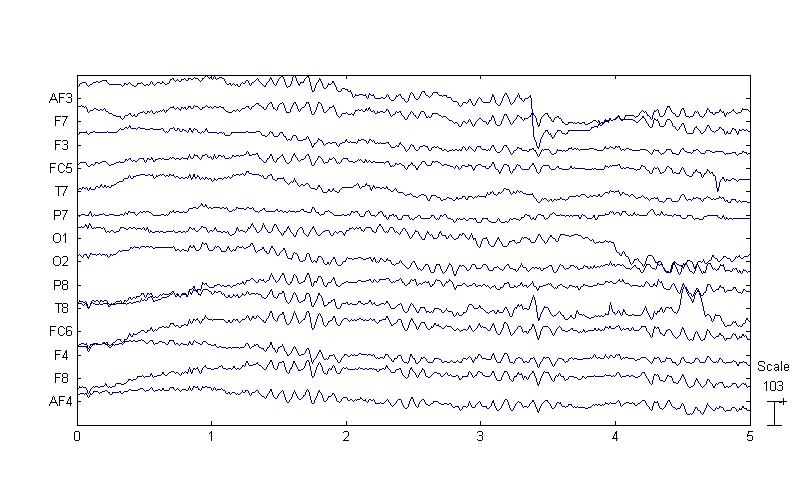
\includegraphics[height=5cm,width=7.5cm]{images/eeglab2.jpg}}
\caption[Alpha Waves Wiggles]{Five seconds of EEG signals obtained from the Emotiv EPOC device.  Fourteen channels are shown.}
\label{fig:alphawavessignals}
\end{figure}

This important rhythm is an oscillatory process.  As such, it is understood and studied in the frequency-domain.   Figure~\ref{fig:alphaspectrum} show the results of applying the Fast Fourier Transform to two different segments of $10\si{\second}$ length.  For each segment, the Power Spectral Density is calculated and their values are shown on the vertical axis.  Frequency values are shown on the horizontal axis.   On Figure (a) no particular frequency component can be spotted.  However, on Figure (b) the prevalence of the 10 \si{\hertz} alpha wave component can be observed.   
 
%As can be seen in Fig. , if we process the Drowsiness dataset with a 8-12Hz band-pass filter and calculate the average power spectral density across subjects and for each channel, we can see how clearly the value corresponding to class 2 (eyes closed) is always higher than the value for class 1 (eyes open), confirming the expected result.  This also verifies how the differentiation information is contained mostly in the frequency-domain.


%(Kamiya 1968) Neurofeedback controlling voluntarily.

\begin{figure}[h!]
\centering
\subfigure[Subject was sit, relaxed in front of the Computer Monitor with his eyes open.]
{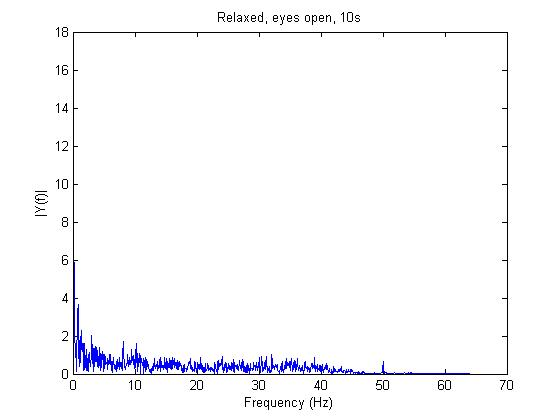
\includegraphics[height=5cm,width=7.5cm]{images/spectrumeyesopenO2.jpg}}
\subfigure[Subject was sit, relaxed in front of the Computer Monitor with his eyes closed. A strong $10 \si{Hz}$ component can be observed.]
{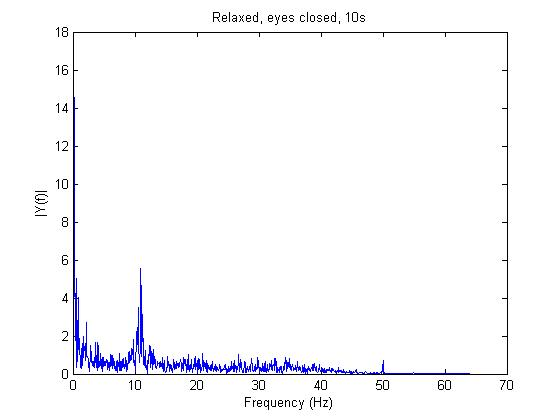
\includegraphics[height=5cm,width=7.5cm]{images/spectrumeyesclosedO2.jpg}}
\caption[Spectrum components obtained by the FFT of Alpha Waves]{Spectrum components of a $10 \si{s}$ signal segment of a subject with their eyes open. Data was obtained with OpenBCI device.}
\label{fig:alphaspectrum}
\end{figure}


%   \begin{figure}[thpb]
%      \centering
%      \setlength\fboxsep{0pt}
%	  \setlength\fboxrule{0.5pt}
%      \fbox{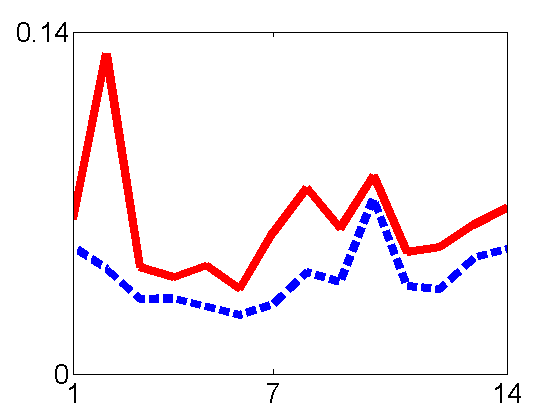
\includegraphics[width=2.5cm, height=1.8cm]{images/PSDExperiment1VsExperiment5.png}}
%      \fbox{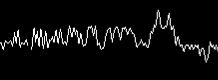
\includegraphics[width=2cm, height=1.8cm]{images/s_1_e_1_c_7_4.png}}
%      \caption[Power Spectral Density of Alpha Waves]{PSD values for every channel (x-axis) are being shown for class 1, dashed line, and class 2, solid line, for Dataset I (left). Sample EEG plot image corresponding to the subject 1 (center) for class 1 (eyes open), for the channel 7 ($ O_1 $) }
%      \label{figure1}
%   \end{figure}
   
\section{Materials and Methods}

This experiments consist in performing a binary classifying of EEG signal segments between the two defined classes.  This will allow to discriminate and identify segments containing significant alpha waves (i.e. eyes closed) from those where these signals are blocked (i.e. eyes open).


\subsection{Emotiv EPOC alpha waves own dataset}
We gather the first dataset using the EEG EPOC Emotiv Headset using the C++ SDK library provided by the manufacturer and an in-house developed software program. The device has 14 channels, and a sampling rate of 128 \si{Hz}\cite{c11}. Ten healthy subjects between ages 20-50 are recruited and they accept to wear the device and to participate in the experiments.  A 30 minutes procedure is required to adjust the headset to each user, in order to decrease the impedance on each electrode (bellow $5 \si{\kilo\ohm}$).  Once the set up is finished, each subject is instructed to sit in a relaxed position. Subsequently, she/he is commanded to watch the screen for 15 seconds, trying to avoid, as much as possible, to abruptly move its body or head.  During that time, a single-trial of 10 seconds-length window of EEG signals data is transferred to a PC and logged into standard binary files. After a 5 minutes pause, the subject is asked to close the eyes avoiding any movement while keeping the same pose for another batch of 15 seconds.  Again, 10 seconds of EEG information are transferred and logged into the PC. This finally produce a sample of 10 subjects,  2 trial per subject, one for each class, composed of 14 channels, 10-seconds length or 1280 samples per window. 

For this dataset, 10 signal segments of 1s for each class were gathered from 10 healthy subjects.  Descriptors were extracted from all the generated images, from both classes, and they were used to classify images from the same set.       
      
\subsection{AlphaNet Dataset}
Additionally, we tested the method against the public dataset of the AlphaNet effort published by Schwartz group.


For the first two datasets, as the sampling frequency of both datasets is similar, Image and SIFT Descriptor Scale were adjusted to delta and gamma to 1.

What is remarkable, and will be is that the information is contained in the frequency domain.  How it was possible to obtain a fairly good accuracy with this method given that important point ?  The key here is the classification algorithm that was used across this thesis.  This is because the local information obtained from each descriptor "help" to balance a tendency of how the synchronous waves all behave, and that information get loaded into the class structure that is later exploited by the classification method.

\subsection{Dataset II - BCI Competition 2003 IV \textit{self-paced 1s}}
We validated our method against the "BCI Competition 2003, dataset IV \textit{self-paced 1s}" \cite{c51}. This dataset is composed of 28 channels, in 416 epochs of 50 samples per epoch (500 ms length at 100 Hz) each one with the corresponding label, where subjects were asked to type at will a letter on a keyboard with the right or left index finger.  It is based on the Bereitschaftspotential \cite{c52}, which is a Slow Cortical Potential, particularly a slow change in voltages towards a negative potential drift, around 1000-500 ms before the onset of the self-initiated movement.  In this case, the information lies strongly on the time-domain.

This dataset was recorded from a healthy subject during a no-feedback session. She/he sat in a normal chair with relaxed arms resting on the table and fingers in the standard typing position at the computer keyboard. The task was to press with the index and little fingers the corresponding keys in a self-chosen order and timing 'self-paced key typing'. The experiment consisted of 3 sessions of 6 minutes each. All sessions were conducted on the same day with some minutes break in-between. Typing was done at an average speed of 1 key per second.  

\section{Results}

As can be seen in Fig. \ref{psd}, if we process the Drowsiness dataset with a 8-12Hz band-pass filter and calculate the average power spectral density across subjects and for each channel, we can see how clearly the value corresponding to class 2 (eyes closed) is always higher than the value for class 1 (eyes open), confirming the expected result.  This also verifies how the differentiation information is contained mostly in the frequency-domain.

We process this Dataset with a 8-12 Hz band-pass filter, and calculate the Power Spectral Density across subjects for each channel.  In Fig. \ref{psd} it can be seen that the PSD value is greater for the class 2 (eyes closed), showing also that the differentiation information is contained mostly in the frequency-domain.

The results of applying a 8-12 Hz band-pass filter and calculating the Power Spectral Density (PSD) across subjects for each channel can be seen in Fig. \ref{figure1}, where the values obtained for class 2 (eyes closed) are higher than the values for class 1 (eyes open), showing that the differentiation information is contained in the frequency-domain.

   \begin{figure}[thpb]
      \centering
      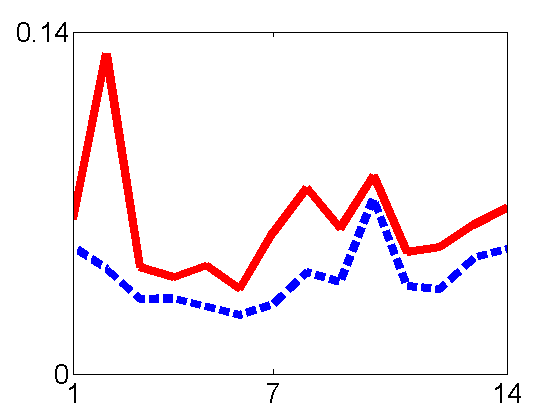
\includegraphics[scale=0.4]{images/PSDExperiment1VsExperiment5.png}
      \caption{Power Spectral Density band-passed at 8-12 Hz, for each channel.  The two experiments shows different levels and it can be seen how the experiment 2 for the Drowsiness Dataset has always higher values.  Channels are numbered according to the device numbering system which corresponds to specific electrodes of the 10-20 international system\cite{c6,c11}. }
      \label{psd}
   \end{figure}
   
   
\begin{figure}[h!]
\centering
\subfigure[10-Fold Cross-validated accuracy values for 10 subjects.  Descriptors were mixed for all the subjects.]
{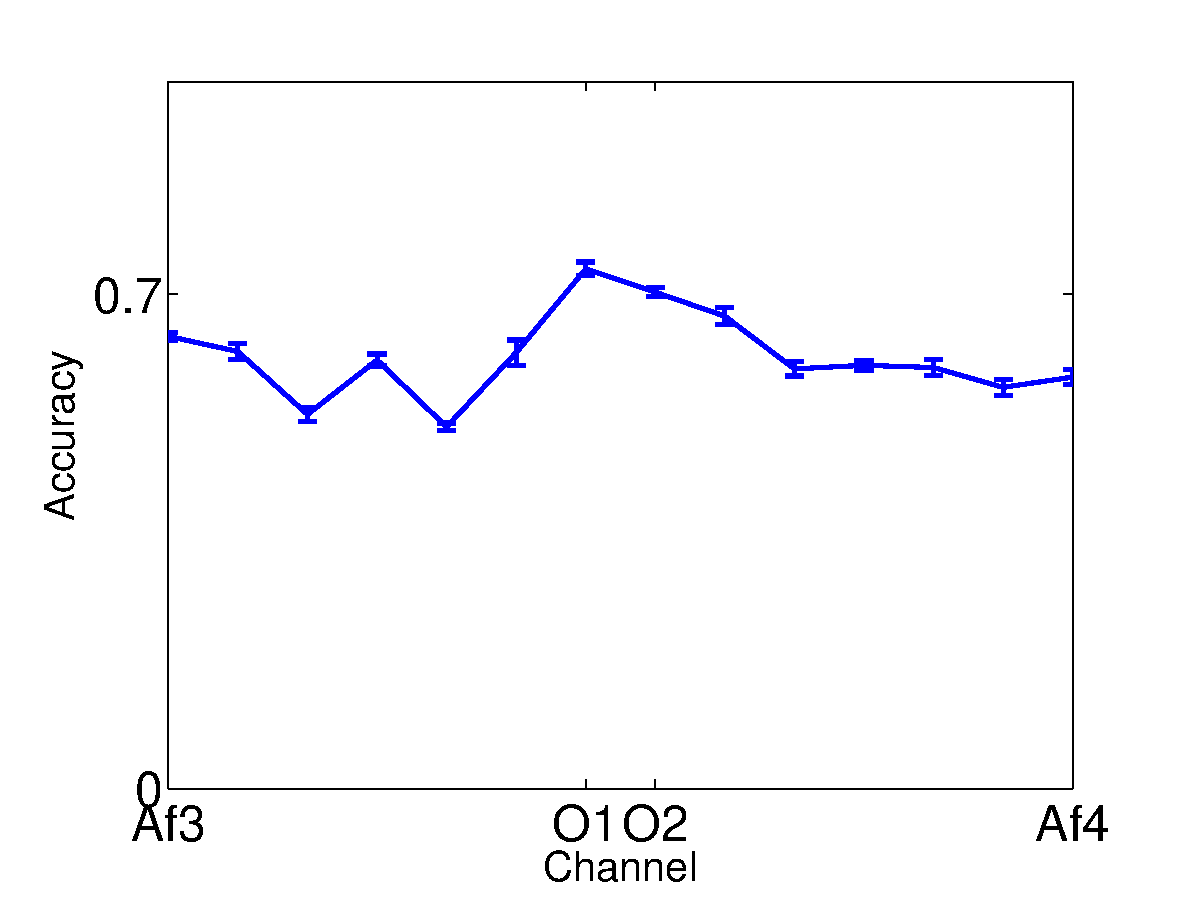
\includegraphics[width=7.5cm, height=5cm]{images/Dataset1AccuracyPerChannel}}
\subfigure[10-Fold Cross-validated accuracies values for subject number 12, using Runs 1 and 2 of the Alphanet Dataset.]
{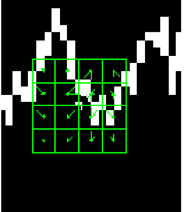
\includegraphics[width=7.5cm, height=5cm]{images/AlphaWaveSampleEEG.png}}
\caption[Alpha Waves Classification]{The classification accuracy is maximum on occipital channels O1 and O2. The descriptor size is 12x12 pixels which corresponds to a variation of 12 microvolts in the signal amplitude during 0.09 s.}
\label{fig:alpharesults}
\end{figure}
   
Regarding the first datasets, results were shown in Fig. 2 (right) where the classification accuracy is shown after applying a 10-Fold Cross Validation procedure on the entire set of labeled descriptors.  Descriptors from different subjects were used as part of the different training set to classify unknown images, so the obtained accuracy level was subject-independent.  Moreover, a classification level with average above $70\%$ was obtained in Occipital channels.


Spatial information based on accuracy

  \begin{figure}[thpb]
      \centering
      \setlength\fboxsep{0pt}
	  \setlength\fboxrule{0.5pt}
      \fbox{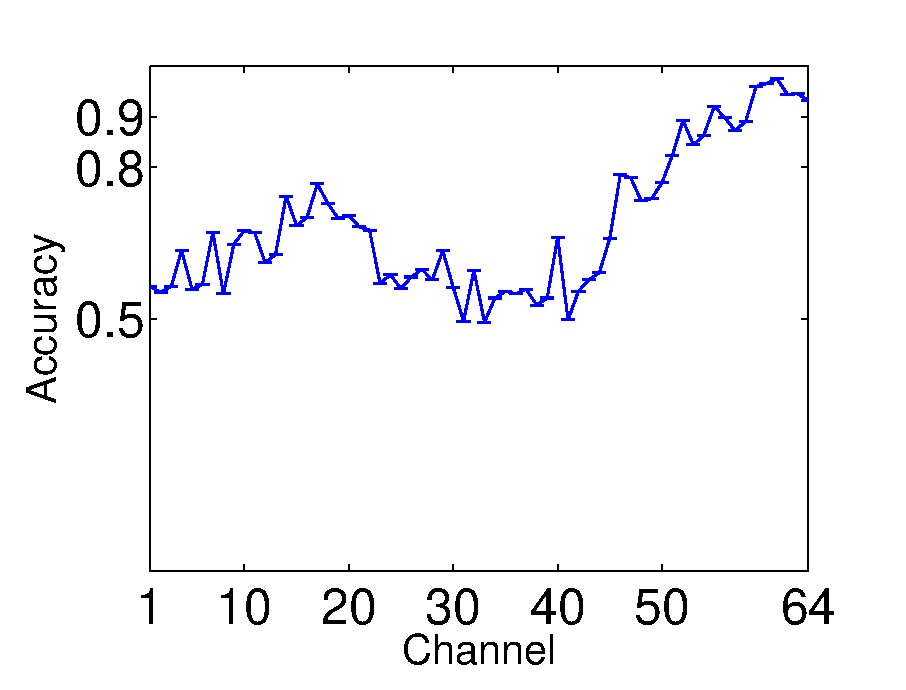
\includegraphics[width=7.5cm, height=5cm]{images/DatasetPhysionetAccuracyPerChannel}}
      \fbox{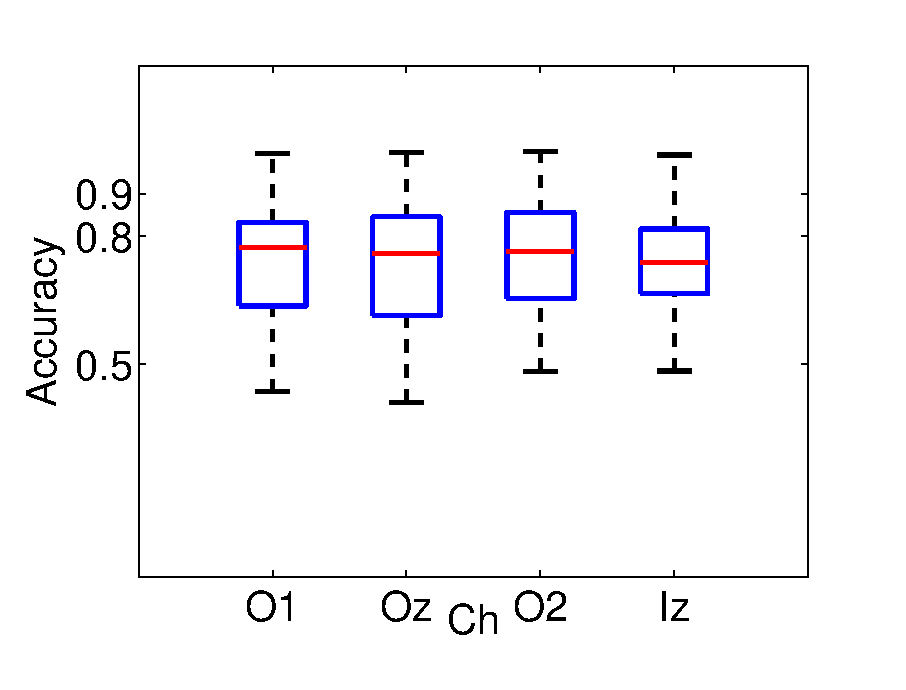
\includegraphics[width=7.5cm, height=5cm]{images/DatasetPhysionetBoxPlots}}
      \caption[Classification Accuracy of Alpha Waves]{}
      \label{figure1}
   \end{figure}   
   
\begin{figure}[h!]
\centering
\subfigure[10-Fold Cross-validated accuracies values for subject number 12, using Runs 1 and 2 of the Alphanet Dataset.]
{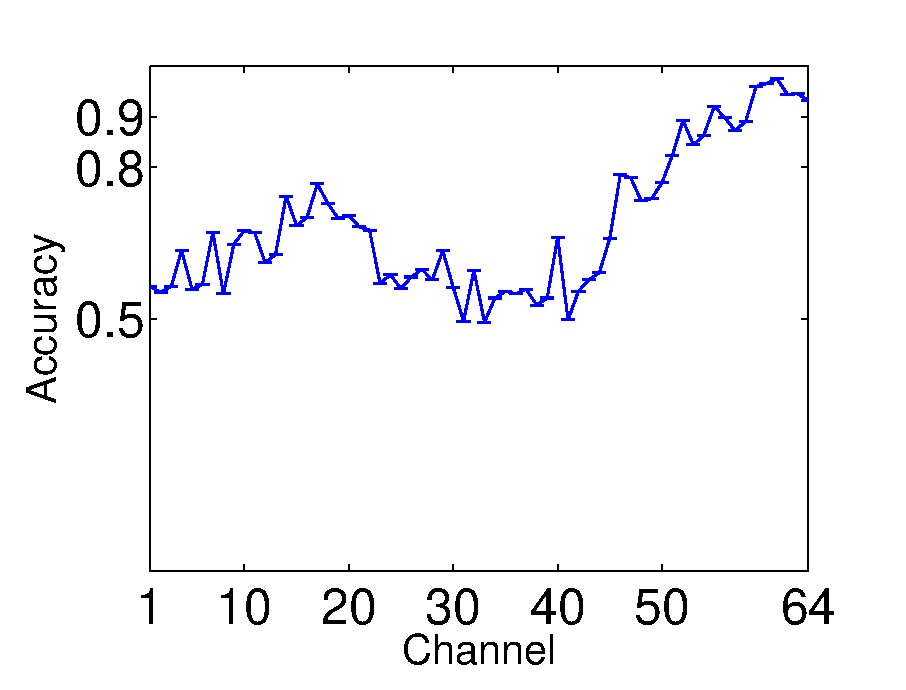
\includegraphics[width=7.5cm, height=5cm]{images/DatasetPhysionetAccuracyPerChannel}}
\subfigure[10-Fold Cross-validated accuracies for O1, Oz, O2 and Iz channels for 25 subjects of the Alphanet Dataset.]
{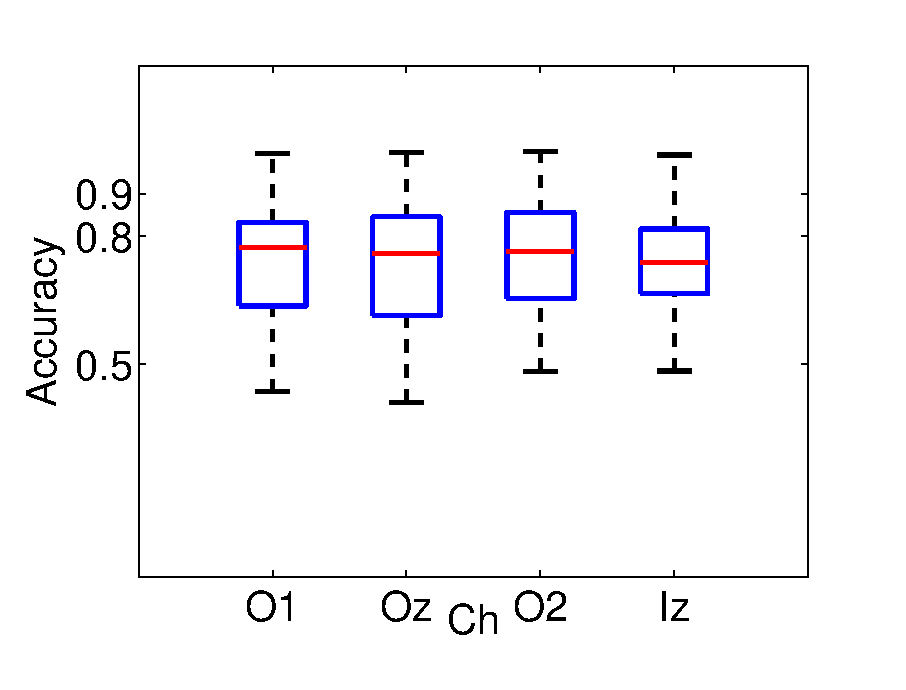
\includegraphics[width=7.5cm, height=5cm]{images/DatasetPhysionetBoxPlots}}
\caption[Alpha Waves Classification]{Classification Accuracy for discriminating windows of 1s (160 samples) of EEG for Alpha Waves differences between subjects with eyes opened and closed. The descriptor size is 12x12 pixels. (Left) 10-Fold cross validated accuracies for one subject.  (Right) Average accuracy levels for 25 subjects for the occipital channels. Medians were above $75\%$.}
\label{fig:alpharesults}
\end{figure}


For the second dataset, an accuracy median higher than $70\%$ for 25 subjects, also on occipital channels O1, Oz, O2 and Iz (numbered 61 to 64) was obtained while discriminating Runs 1 and 2 (Baseline eyes open vs Baseline eyes closed). Fig. 3 shows the 10-Fold Validated Accuracy for one random subject [6,7], where a higher accuracy in the classification of the signals can also be seen with occipital channels.  

\section{Conclusion}

This results was surprassing.  We are using a method which is based on the waveform do detect a process which happens to be more prominent in spectrum.  But this shows at the same time the complex relationshipt between time and frequency.  The shape in time of a an oscilatory process prominent in frequency is clearly evident.  This goes in line with the fact that alpha waves can be seen in the EEG, and are basic tools of clinical diagnosis.

The posterior rythm is very important to assess healthy EEG patterns.


Although EPOC Emotiv is a commercial device, more apt as HCI tool, it is possible to detect fairly some BCI components.

Covert Spatial visual Attention


Offline Alpha Waves presence was detected from signal plot with an accuracy level 10-fold cross validated of 70\%.
\chapter{Alpha Wave: spotting wiggles}
\label{chapter:four}
\epigraph{The electroencephalogram represents a continuous curve with continuous oscillations in which... one can distinguish larger first order waves with an average duration of 90 milliseconds...}{Berger}

This Chapter describes the experiments performed over a well-established but still mysterious EEG cognitive signal: The Berger Rhythm or Visual Occipital Alpha Waves.  An own dataset of resting subjects with and without alpha blocking is produced and the details of their generation are outlined.  Additionally, an experiment on a public dataset is also delineated.  Conclusions and discussion are described in the last section.

\section{Introduction}

%We gather the first dataset  using the EEG EPOC Emotiv Headset and we  access the raw signals using its C++ SDK provided by the manufacturer.  The device sends wirelessly  digitalized 128 Hz sampled EEG information as discrete packets.  Every packet is numbered and the electronic impedance is constantly measured, and delivered as part of the packet information. The wireless transmitter connects to a standard RF dongle which receives the information from  14 channels and forwards it into the PC, particularly to a custom C++ EEG Datalogger program that was developed in-house.  The program is waiting passively until a new packet is received from the dongle, verifying the packet numbering and controlling that the impedance is bellow a certain level, according to the device's documentation \cite{Stopczynski2014}. 

Alpha Waves were the first signals ever spotted from the Electroencephalography.  They are regularly characterized as $10\si{Hz}$, or more broadly between the frequency band of $8$-$12$ $\si{Hz}$. They are physiologically consistent across subjects, though it has been reported inter- and intra- variations with functional cognitive implications~\cite{Haegens2014}.   Moreover, they are associated with synchronous inhibitory processes and attention shifting~\cite{Sanei2007}. They tend to be more prominent while subject's eyes are closed and appear stronger in occipital regions, around $O_1$ and $O_2$~\cite{WolpawJonathanR2012,Stopczynski2014}. These waves are also called Prominent Posterior Alpha or Posterior Dominant Rhythm due to their pervasiveness in EEG~\cite{Schomer2010,Haegens2014}.

Figure~\ref{fig:alphawavessignals} shows two records of 8-channels signals.  Figure ~\ref{fig:alphawavessignals}(a) contains the registered alpha waves of a subject with their eyes open while the (b) contains the same information with their eyes closed.  The characteristic pattern of wiggles can be spotted in the latter, while their absence entails the blocking of alpha waves in the former~\cite{Basar2012}. 


\begin{figure}[h!]
\centering
\subfigure[EEG signals of a relaxed healthy subject with their eyes open.]
{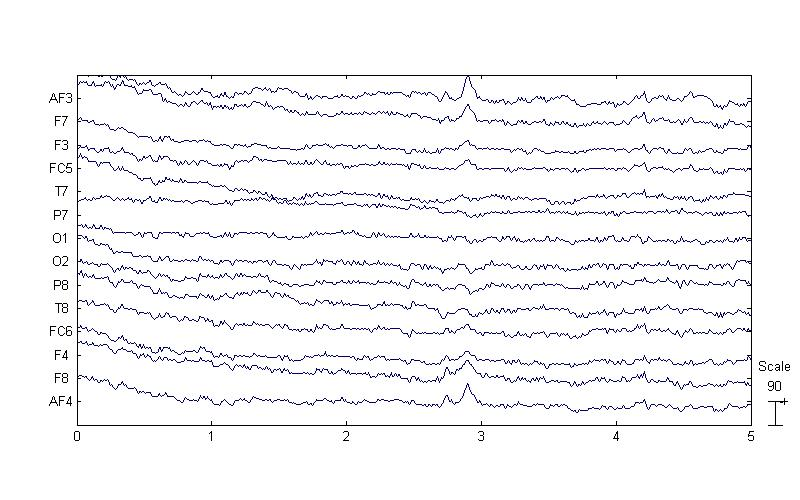
\includegraphics[height=5cm,width=7.5cm]{images/eeglab1.jpg}}
\subfigure[EEG signals of the same relaxed subject with their eyes closed. Alpha Waves wiggles can be spotted since the first second.]
{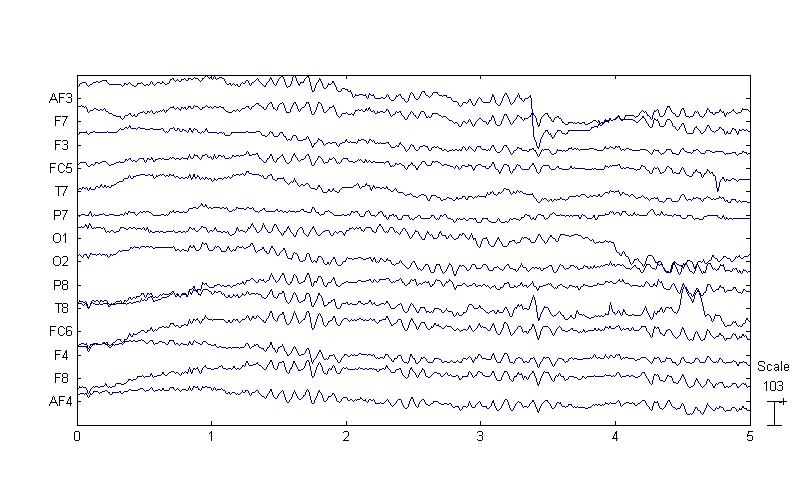
\includegraphics[height=5cm,width=7.5cm]{images/eeglab2.jpg}}
\caption[Alpha Waves Wiggles]{Five seconds of EEG signals obtained from the Emotiv EPOC device.  Fourteen channels are shown on the vertical axis, while x-axis shows time in seconds.}
\label{fig:alphawavessignals}
\end{figure}

This important rhythm is an oscillatory process.  As such, it is understood and studied in the frequency-domain.   Figure~\ref{fig:alphaspectrum} shows the results of applying the Fast Fourier Transform to two different segments of $10\si{\second}$ length.  For each segment, the power spectral density is calculated and their values are shown on the vertical axis.  Frequency values are shown on the horizontal axis.   On Figure~\ref{fig:alphaspectrum}(a) no particular frequency component can be spotted.  However, on Figure~\ref{fig:alphaspectrum}(b) the prevalence of the 10-\si{\hertz} alpha wave component can be observed.   
 
%As can be seen in Fig. , if we process the Drowsiness dataset with a 8-12Hz band-pass filter and calculate the average power spectral density across subjects and for each channel, we can see how clearly the value corresponding to class 2 (eyes closed) is always higher than the value for class 1 (eyes open), confirming the expected result.  This also verifies how the differentiation information is contained mostly in the frequency-domain.


%(Kamiya 1968) Neurofeedback controlling voluntarily.

\begin{figure}[h!]
\centering
\subfigure[Subject was sit, relaxed in front of the Computer Monitor with his eyes open.]
{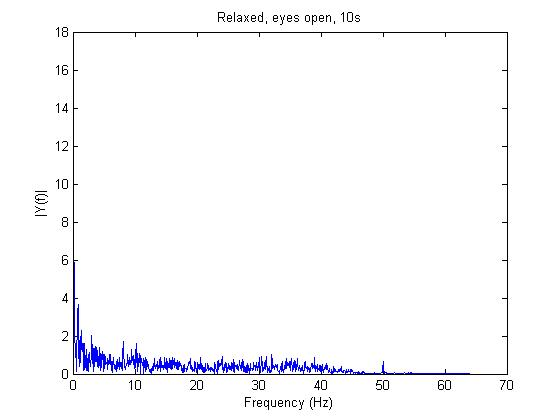
\includegraphics[height=5cm,width=7.5cm]{images/spectrumeyesopenO2.jpg}}
%{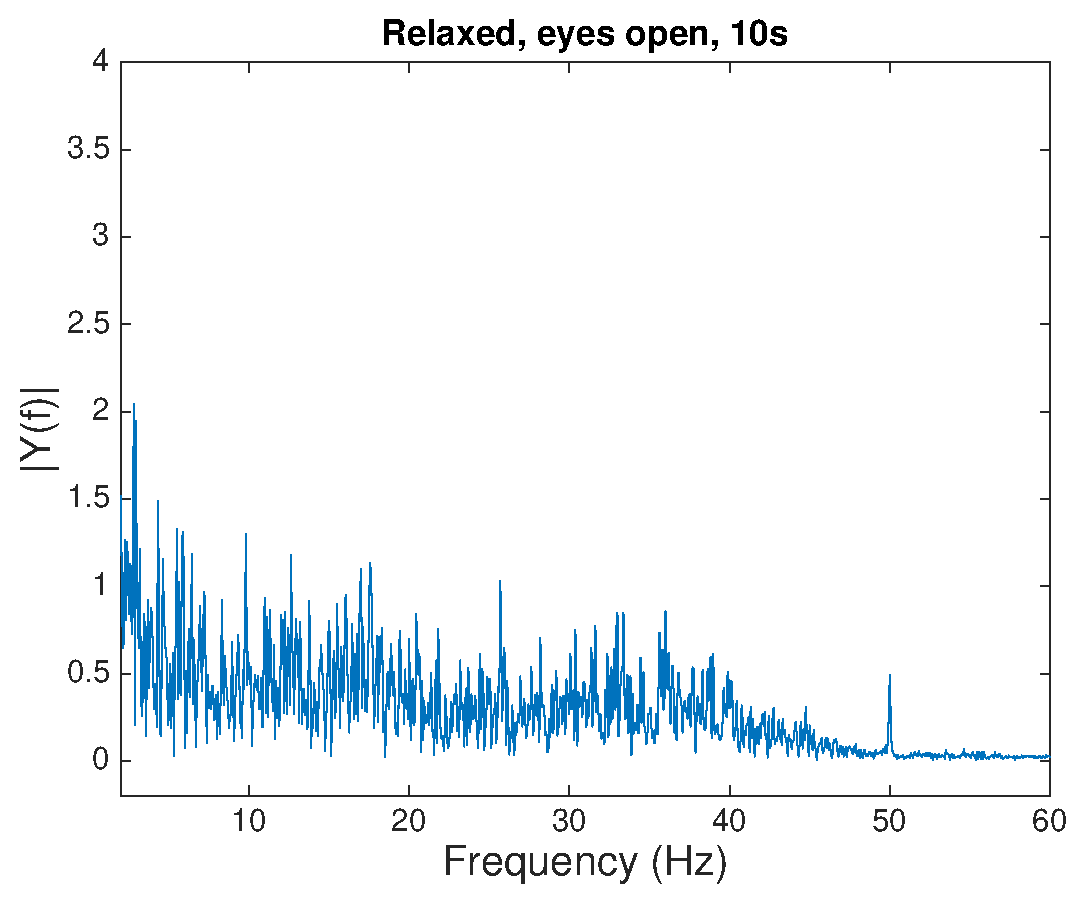
\includegraphics[height=5cm,width=7.5cm]{images/eyesopen.eps}}
\subfigure[Subject was sit, relaxed in front of the Computer Monitor with his eyes closed. A strong $10 \si{Hz}$ component can be observed.]
{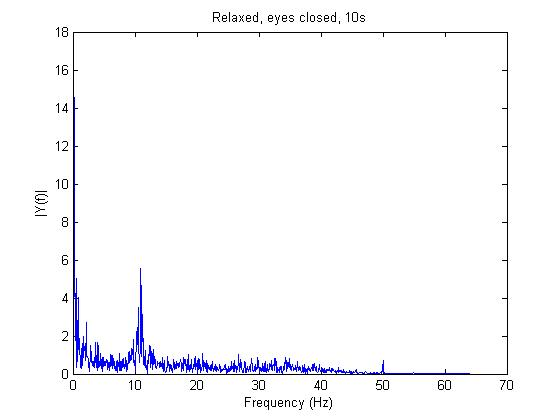
\includegraphics[height=5cm,width=7.5cm]{images/spectrumeyesclosedO2.jpg}}
%{\includegraphics[height=5cm,width=7.5cm]{images/eyesclosed.eps}}
\caption[Alpha Waves Spectrum Components]{Spectrum components of a $10 \si{s}$ signal segment of a subject with their eyes open. Horizontal axis shows different frequencies while the vertical axis represents the power spectral density.  In both diagrams a $50 \si{Hz}$ line component can be visualized.} 
\label{fig:alphaspectrum}
\end{figure}


%   \begin{figure}[thpb]
%      \centering
%      \setlength\fboxsep{0pt}
%	  \setlength\fboxrule{0.5pt}
%      \fbox{\includegraphics[width=2.5cm, height=1.8cm]{images/PSDExperiment1VsExperiment5.png}}
%      \fbox{\includegraphics[width=2cm, height=1.8cm]{images/s_1_e_1_c_7_4.png}}
%      \caption[Power Spectral Density of Alpha Waves]{PSD values for every channel (x-axis) are being shown for class 1, dashed line, and class 2, solid line, for Dataset I (left). Sample EEG plot image corresponding to the subject 1 (center) for class 1 (eyes open), for the channel 7 ($ O_1 $) }
%      \label{figure1}
%   \end{figure}
   
\section{Materials and Methods}

These experiments consist in performing a binary classification of EEG signal segments between the two defined classes.  Class 2 is assigned to segments containing significant alpha waves (i.e. eyes closed), whereas class 1 identifies those where these signals are blocked (i.e. eyes open).


\subsection{Dataset I - Emotiv EPOC alpha waves own dataset}
\label{dataset1}
The first dataset is gathered using the EEG EPOC Emotiv Headset.  Although this is a commercial-grade device, it provides an acceptable price-performance ratio and it has been used to investigate basic EEG processes~\cite{Debener2012,DeVos2014}. In order to obtain the multichannel raw EEG signal, a C++ SDK library provided by the manufacturer is used and an in-house software program is developed. This device has 14 channels, and a sampling rate of 128 \si{Hz}~\cite{Stopczynski2014}. Available channels are AF3, F7, F3, FC5, T7, P7, O1, O2, P8, T8,  FC6, F4, F8, AF4.  Ten healthy subjects between ages 20-50 are recruited and they accept to wear the device and to participate in the experiments.  

A 30 minutes procedure is required to adjust the headset to each user, in order to decrease the impedance on each electrode (below $5 \si{\kilo\ohm}$).  
This is achieved by physically adjusting the headset position over the scalp, and by embedding each electrode electrode pad in saline solution.
A software program developed by the manufacturer is used to obtain the measured impedance.  Once the set up is finished, each subject is instructed to sit in a relaxed position. Subsequently, she/he is commanded to watch the screen for 15 seconds, trying to avoid, as much as possible, to abruptly move its body or head.  During that time, a single-trial of 10 seconds-length window of EEG signals data is transferred to a PC and logged into standard binary files. After a 5 minutes pause, the subject is asked to close the eyes avoiding any movement while keeping the same pose for another batch of 15 seconds.  Again, 10 seconds of EEG information are transferred and logged into the PC. This finally produces a dataset of 10 subjects,  2 classes per subject, composed of 14 channels, 10-seconds length or 1280 samples per window.  These windows are further divided into 10 segments per class and per subject.

%\begin{figure}[thpb]
%\centering
%\setlength\fboxsep{0pt}
%\setlength\fboxrule{0.5pt}
%\fbox{\includegraphics[width=3.5cm, height=2.5cm]{images/emotivlarge.png}}
%\fbox{\includegraphics[width=3.5cm, height=2.5cm]{images/emotivpositions.png}}
%\fbox{\includegraphics[width=3.5cm, height=2.5cm]{images/emotivcalibration.png}}
%\fbox{\includegraphics[width=3.5cm, height=2.5cm]{images/emotivdatasetsubject.jpg}}
%\caption[Classification Accuracy of Alpha Waves]{}
%\label{figure1}
%\end{figure}   
   
\begin{figure}[h!]
\centering
\subfigure[]
{\includegraphics[width=3.5cm, height=3cm]{images/emotivlarge.png}}
\subfigure[]
{\includegraphics[width=3.5cm, height=3cm]{images/emotivpositions.png}}
\subfigure[]
{\includegraphics[width=3.5cm, height=3cm]{images/emotivcalibration.png}}
\subfigure[]
{\includegraphics[width=3.5cm, height=3cm]{images/emotivdatasetsubject.jpg}}
\caption[EPOC Emotiv Alpha Waves Dataset]{(a) EPOC Emotiv consumer-grade 14-channels wireless EEG.(b) This device has a fixed set of positions according to the 10-20 International System.(c) While resting and sitting confortable in a chair, subjects had to fixate their sight to the center of this image which was being displayed on a computer monitor, 1 \si{meter} away from the subject.(d) Subject performing the experiment to produce the dataset described in \ref{dataset1}.}.
\label{fig:alpharesults}
\end{figure}

\begin{story}[Measuring BCI Performance]
Measuring the performance of the BCI system as it is described in the model of Figure~\ref{fig:bciblockdiagram} is of quite relevance in the field.  The term \textit{Accuracy} in BCI refers in general to binary classification accuracy, which means how many bit predictions between two different classes and on unlabeled data is the BCI classifier able to perform correctly.  This is the metric that is being used in this Chapter.  Other metrics include Cohen Kappa (used to measure agreements between different experts), Recall (sensitivity), Specificity, Precision and F-Score~\cite{Nicolas-Alonso2012,Chavarriaga2017,c55,WolpawJonathanR2012,Clerc2016,Nam2018}. At the same time, the theoretical chance level is a related concept that determines what will be the outcome if the classifier is just randomly selecting one choice~\cite{Nam2018}.  For binary classification this value is $50\%$ when datasets are balanced~\cite{Tibon2015}.  For unbalanced data the Receiving Operating Characteristics (ROC) curve helps to understand and compare better the predictive efficiency of the classifier~\cite{Fawcett2006}. For more practical systems, like P300-Based BCI Spellers, it is preferred a measure of the plain performance of the system to achieve the task at hand (e.g. like character recognition rates)~\cite{Krusienski2006}. When the interface aspect of the system is remarked, or when the communication speed is of relevance, the Information Transfer Rate (ITR) or Bit Transfer Rate (BTR) is used to provide a metric on the amount of bits that it is possible to extract from the BCI system to transmit information.

Despite all this, the best metric is the one provided from real users using a robust system or from clinicians using a helpful tool~\cite{Huggins2015,Nijboer2009,c56}.

\end{story}
      
\subsection{Dataset II - AlphaNet Dataset}
Additionally, the performance of HIST was tested against the public dataset EEG Motor Movement/Imagery Dataset of the PhysioNet effort published and mantained by the U.S. National Health Service~\cite{Schalk2004,Goldberger2000}.  

Baseline records and motor/imagery tasks were performed by 109 healthy volunteers, using the BCI2000 system~\cite{Schalk2004} at a sampling frequency $\gls{Fs} = 160$.  At the same time 64-channel EEG records were registered where each subject completed 14 tasks, called Runs.  The first two are the baseline calibration tasks, of relevance for this Chapter.  These Runs 1 and 2 are each one-minute records of resting subjects with eyes open and eyes closed.  From these records, 60 segments of 1-second length are further extracted per subject. Class labeling is the same as Dataset I.  The experiment was performed on 25 randomly selected subjects out of the 109.


%This dataset
%
%Subjects performed different motor/imagery tasks while 64-channel EEG were recorded using the BCI2000 system (http://www.bci2000.org). Each subject performed 14 experimental runs: two one-minute baseline runs (one with eyes open, one with eyes closed), and three two-minute runs of each of the four following tasks:
%
%A target appears on either the left or the right side of the screen. The subject opens and closes the corresponding fist until the target disappears. Then the subject relaxes.
%A target appears on either the left or the right side of the screen. The subject imagines opening and closing the corresponding fist until the target disappears. Then the subject relaxes.
%A target appears on either the top or the bottom of the screen. The subject opens and closes either both fists (if the target is on top) or both feet (if the target is on the bottom) until the target disappears. Then the subject relaxes.
%A target appears on either the top or the bottom of the screen. The subject imagines opening and closing either both fists (if the target is on top) or both feet (if the target is on the bottom) until the target disappears. Then the subject relaxes.

\subsection{Parameters}

Images and plots are generated according to Section~\ref{Plot}, with an autoscale plotting scheme.  Keypoint localization is determined according to Section~\ref{keypointlocation} by following the trace of the signal, with a $\gls{kpd} = 1$.   Descriptors are extracted from all the generated images, from both classes, and they are used to classify images in a 10-fold cross-validation procedure.  The classification method described in Section~\ref{nbnn} is used to perform a binary classification.  The parameter $\gls{gamma}$ is set to $2$, as well as $\gls{gammat}$.  

%For the first two datasets, as the sampling frequency of both datasets is similar, Image and SIFT Descriptor Scale were adjusted to delta and gamma to 1.

%\subsection{Dataset III - BCI Competition 2003 IV \textit{self-paced 1s}}
%We validated our method against the "BCI Competition 2003, dataset IV \textit{self-paced 1s}" \cite{c51}. This dataset is composed of 28 channels, in 416 epochs of 50 samples per epoch (500 ms length at 100 Hz) each one with the corresponding label, where subjects were asked to type at will a letter on a keyboard with the right or left index finger.  It is based on the Bereitschaftspotential \cite{c52}, which is a Slow Cortical Potential, particularly a slow change in voltages towards a negative potential drift, around 1000-500 ms before the onset of the self-initiated movement.  In this case, the information lies strongly on the time-domain.
%
%This dataset was recorded from a healthy subject during a no-feedback session. She/he sat in a normal chair with relaxed arms resting on the table and fingers in the standard typing position at the computer keyboard. The task was to press with the index and little fingers the corresponding keys in a self-chosen order and timing 'self-paced key typing'. The experiment consisted of 3 sessions of 6 minutes each. All sessions were conducted on the same day with some minutes break in-between. Typing was done at an average speed of 1 key per second.  

\section{Results}

Dataset I was controlled and verified by processing it with a 8-12Hz band-pass filter, and calculating the average power spectral density across subjects for all channels.  It can be observed on Figure \ref{fig:psd}(a)  that values corresponding to class 2 (eyes closed) are always higher than the values obtained for class 1 (eyes open). On the other hand, for the sake of illustration, a scatter plot of the obtained segment's power spectral density for O1 vs O2 for Subject 2 is shown, where a separation of classes can be devised.  This proves that there is discriminative information in the frequency-domain.



\begin{figure}[h!]
\centering
\subfigure[Power spectral density averaged across 10 subjects for each channel. Values for Class 2 (red) are always higher than values for Class 1 (blue).]
{\includegraphics[width=7.5cm, height=5cm]{images/PSDExperiment1VsExperiment5.png}}
\subfigure[Scatterplot of power spectral density for the channel O1 vs O2.  There is a separation of classes between the red (class 2) and blue(class 1) dots.]
{\includegraphics[width=7.5cm, height=5cm]{images/alphawavesscatterpsd.png}}
\caption[Power Spectral Density of the Dataset I]{Frequency analysis of Dataset I}
\label{fig:psd}
\end{figure}
   
Results of applying the 10-fold cross validation procedure on the entire set of labeled descriptors is shown on Figure~\ref{fig:alpharesultsdataseti}. Template dictionaries for class 1 and class 2 are formed using training descriptors for all the subjects at the same time.  Hence, the testing step of the cross-validation procedure is implemented subject by subject, but performing a transfer learning between subjects. The classification is subject-independent, and an averaged accuracy across all subjects is above $70\%$, obtained in occipital channels.
   
\begin{figure}[h!]
\centering
\subfigure[Ten-fold cross-validated accuracy values, averaged across $10$ subjects.  Descriptors used for calibration are intermixed to create one template dictionary which is used for all subjects.]
{\includegraphics[width=7.5cm, height=5cm]{images/Dataset1AccuracyPerChannel}}
\subfigure[Amplified image containing a sample patch located on one of the images generated for one 1-second long segment of this dataset. The keypoint location is on a sample point along the EEG trace.]
{\includegraphics[width=7.5cm, height=5cm]{images/AlphaWaveSampleEEG.png}}
\caption[Dataset I Classification Rate]{Dataset I: The classification accuracy is maximum on occipital channels O1 and O2. The horizontal patch scale $\gls{St}$ and the vertical patch scale $\gls{Sv}$ are set to $1$, whereas $\gls{gamma}$ and $\gls{gammat}$ are set to $2$, which corresponds to a variation of $\gls{DeltamuV} = 10$ microvolts in the signal amplitude during $\gls{lambda}=0.08$ $\si{seconds}$.}
\label{fig:alpharesultsdataseti}
\end{figure}

% Hay que traducir todo eso a los nuevos simbolos.
   

%  \begin{figure}[thpb]
%      \centering
%      \setlength\fboxsep{0pt}
%	  \setlength\fboxrule{0.5pt}
%      \fbox{\includegraphics[width=7.5cm, height=5cm]{images/DatasetPhysionetAccuracyPerChannel}}
%      \fbox{\includegraphics[width=7.5cm, height=5cm]{images/DatasetPhysionetBoxPlots}}
%      \caption[Classification Accuracy of Alpha Waves]{}
%      \label{figure1}
%   \end{figure}   
   
\begin{figure}[h!]
\centering
\subfigure[Ten-fold cross-validated accuracy boxplots for O1, Oz, O2 and Iz channels, for the 25 subjects. Mean values are around $70\%$.]
{\includegraphics[width=7.5cm, height=5cm]{images/DatasetPhysionetBoxPlots}}
\subfigure[Ten-fold cross-validated accuracies values for a randomly selected subject (number 12), using runs 1 and 2.]
{\includegraphics[width=7.5cm, height=5cm]{images/DatasetPhysionetAccuracyPerChannel}}
\caption[PhysioNet Dataset Binary Classification Accuracy]{Dataset II: Classification Accuracy for segments of 1s ($\gls{N} = 160$) of EEG, between class 1 and class 2.  In this case as the sampling frequency $\gls{Fs}$ is lower, the signal span is $\gls{lambda} = 0.06$   $\si{s}$}.
\label{fig:alpharesultsdatasetii}
\end{figure}


For the Dataset II, training and testing steps of the cross-validation procedure are implemented subject by subject.  An averaged accuracy across 25 subjects of around $70\%$ is obtained, also on occipital channels O1, Oz, O2 and Iz (numbered 61 to 64) while discriminating runs 1 versus 2 (baseline eyes open vs baseline eyes closed).  This information can be devised on Figure~\ref{fig:alpharesultsdatasetii}(a) where boxplots of the accuracies for these four occipital channels and for all the 25 subjects, are represented.  On the other hand, Figure~\ref{fig:alpharesultsdatasetii}(b) shows the 10-fold validated accuracy for one random subject. A higher accuracy in the classification of the signals can also be seen over occipital channels.

\section{Conclusion}

It is known and it was verified here that the discriminative information in EEG alpha waves is mostly contained in the frequency-domain.  In spite of this,  there is enough information encoded in the alpha waves wiggles to classify signal segments solely on the \textit{features} captured by the HIST method, proposed in this Thesis.  

It was also verified that the presence of oscillatory alpha waves is higher around occipital regions and that an automated procedure which analyze visually the image structure can detect them. This important oscillatory rhythm has many connections with shifting of attention and with volitional changes and is of quite relevance in BCI research~\cite{Basar2012}.  Particularly, the BCI paradigm of Visual Spatial Covert Attention is a further area of research for this method due to the fact that it is entirely based on analyzing alpha waves~\cite{vanGerven2009}. Moreover, the posterior rythm has many implications outside the field of BCI and is very important to assess healthy EEG patterns. The exact meaning of alpha waves is still debated~\cite{Ahn2013} and this basic procedure can open the possibility to explore it under a different perspective and verify if they can be effectively tied to some unexpected form of volitional control which may be effective for BCI understanding and improvement.

%The key here is the classification algorithm that was used across this thesis.  This is because the local information obtained from each descriptor "help" to balance a tendency of how the synchronous waves all behave, and that information get loaded into the class structure that is later exploited by the classification method.
%
%This results was surprassing.  We are using a method which is based on the waveform do detect a process which happens to be more prominent in spectrum.  But this shows at the same time the complex relationshipt between time and frequency.  The shape in time of a an oscilatory process prominent in frequency is clearly evident.  This goes in line with the fact that alpha waves can be seen in the EEG, and are basic tools of clinical diagnosis.

%Although EPOC Emotiv is a commercial device, more apt as HCI tool, it is possible to detect fairly some BCI components.





\chapter{Motor Imagery: the hunt for a greek letter}
\label{chapter:five}
\epigraph{...utilizing the brain signals in man-computer dialogue.}{Vidal}

\section{Introduction}

Motor Imagery is an EEG or ECoG based BCI paradigm originated on changes of SMR, sensorimotor rhythms, that are altered when a person engages in motor behavior, but it can also be elicited when a person imagines to perform any movement. Particularly, the Rolandic wicket rhythm, the $\mu$ rhythm, is of the same frequency (e.g. 8-12 Hz) of visual occipital alpha waves, but from a spatially different location (posterior frontal and anterior parietal areas)\cite{WolpawJonathanR2012}.   Although SMR patterns presents a high inter- and intra-subjects variability regarding the signal features required to identify them, an Event Related Desynchronization/Synchronization of $\mu$ rhythm is in general consistent across subjects, regardless of the specificity of the imagined movement (i.e. what is being imagined to move).

\section{Materials and Methods}

In order to verify if this ERD/ERS could be detected by the method presented in this Thesis, i.e. by automatically extracting the information from the signal plots, a BCI Simulation is performed against the public Motor Imagery Dataset 002-2014, published by BNCI-Horizon 2020 website and initiative~\cite{Steyrl2015}.  This dataset is composed of 8 runs for 14 participants, aged between 30 and 30 years, five females, with a sampling frequency of $\gls{Fs} = 512$. Nine out of these 14 participant reported never been exposed to a BCI device.  One session per participant is recorded on a single day and one session consisted of eight consecutive runs with short pauses between them.  The first 5 runs are used for training without feedback, and the remaining 3 runs are used to test the results.  The original online experiment was performed with 20 trials on each run, 10 corresponding to imagining moving the right hand and the other 10 to feet movement.  Figure~\ref{fig:midatasetdiagram} schematize the protocol and the structure of this published dataset.  This BCI simulation experiment is divided in two.  In the first simulation, baseline signals, corresponding to the 1st second of each trial are compared against right hand motor imagery, which is 4.5 seconds ahead of the beginning of each trial. Signal segments of 1-second length are processed for 10 trials for each of 5 runs and their descriptors are extracted for both classes.  The second BCI simulation is similar but only extracting trials corresponding to feet movement imagery.



\begin{story}[BCI Simulation or Cross Validation?]
The task of decoding information from brain signals inherits practices from Machine Learning.  Cross-Validation is used in ML to reduce overfitting bias and to increase the independence on the dataset that is used as calibration (see Section~\ref{Calibration}).  However, the brain signals used in BCI are extracted from a person who is performing a task and whose signals are changing while trying to adapt to this operation.  Hence, mixing the dataset, shuffling the sessions and trials is at least a challenging assumption.  BCI Simulation, on the other hand, is not very well defined in BCI research, but their practice, without naming it, has been the regular approach for BCI Competitions. It consists in reproducing the operational sequence that was used to generate the dataset. The offline the experiment is replicated, using the training information to train or calibrate a classifier, and to classify the signals as if they were generated at that same moment.

Regardless, of any definition, the online validation with feedback of any BCI system is the unquestioned gold standard of the discipline~\cite{WolpawJonathanR2012}.
\end{story}


\begin{figure}[]
\centering
\includegraphics[scale=0.6]{images/DatasetIIIDiagram2.png}
\caption[Motor Imagery Experimental Protocol]{Fourteen voluntary Participants performed 5 sessions of training and 3 sessions of testing.  On each session each subject had 10 trials to perform Right Hand Motor Imagery and 10 trials for Feet Movement.  At the same time, each trial has a 2-seconds baseline and a 4-seconds section to perform the imagery task.  For each BCI Simulation, Class 1 is defined from EEG information obtained from the baseline section, while Class 2 is based on extracting segments from the imagery section of the EEG signal.}
\label{fig:midatasetdiagram}
\end{figure}


\section{Results}

Binary classification accuracies are calculated based on the output of the BCI simulation on the remaining 3 runs for each participant, in a single-trial approach: for each sampled segment of 1-second length, classification based on the classification algorithm described in \ref{nbnn} is applied and a match or mismatch is obtained.  Results are shown in Figure~\ref{fig:miresults} where for right-hand detection \textit{RH}, average accuracies of around $70\%$ are obtained for the channel C3, the best-performing channel $\gls{bpc}$, coincidentally with the contralateral structure of the imagined movement.  On the other hand, the binary classification accuracy for feet imagery detection \textit{FM}, achieves in all the channels accuracies of just above chance level.

%TODO Theoretical chance level from the NAM book of lotte.
   
\begin{figure}[h!]
\centering
\subfigure[]
{\includegraphics[width=7cm, height=5cm]{images/MIinformedonpaper1.png}}
\subfigure[]
{\includegraphics[width=7cm, height=5cm]{images/MIinformedonpaper2.png}}
\caption[Motor Imagery Accuracy]{Classification Accuracy for discriminating segments of 1s ($\gls{N} = 512$) of EEG for Motor Imagery detection BCI simulation. (a) Accuracy values for channels C3, Cz and C4 for the 14 participants of the described MI dataset discriminating between baseline and right-hand imagery. (b)The same procedure for feet imagery. Accuracy levels averaged to $70\%$ are obtained only for right-hand movement on the contralateral channel C3. The horizontal $\gls{St}$ and vertical $\gls{Sv}$ patch scale are adjusted to $6$}.
\label{fig:miresults}
\end{figure}

%TODO Agregar bien cual es la conversion en pixeles que se obtiene y probarlo.
   
\section{Conclusion}

Offline BCI Simulation of single trial asynchronous triggering for right hand MI based on signal plots is implemented with a level of success of $70\%$ for 7 out of 14 Participants. Single trial asynchronous triggering of BCI can be implemented with this paradigm, particularly for right-hand motor imagery. The name $\mu$ rhythm was precisely coined because the shape of the waves have some resemblance to the greek letter~\cite{Cole2017}.   Additionally, in line with previous chapter results, though the differentiation information is contained in the frequency domain, the method based on the Histogram of Gradient Orientation detected differences in the shape of the signals.  Coincidentally with results obtained from Alpha Waves, there is information that is mapped in the structure of the waveform, at least for frequencies on the 10 Hz range, which characterize both types of waves.

% Parameters
% Poner una figura donde más o menos se vean las señales.



\chapter{Conclusions}

BCI Security (IEEE Paper Life Science)



Sleep staging is one of the most important steps in sleep analysis. It is
a very time consuming task consisting of classifying all 30 second pieces
of an approximately eight hour recording into one of six sleep stages:
wakefulness, S1 (light sleep), S2, S3, S4 (deep sleep), REM (rapid eye
movement) sleep. A sleep recording is made with a minimum setting
of four channels: electro-encephalogram (EEG) from electrodes C3 and
C4 1, electro-myogram (EMG) and electro-oculogram (EOG). 

In order
to classify each 30 second segment of sleep according to the classical
[Rechtschaen  Kales 1968] (RK) rules, the human scorer looks for
defined patterns of waveforms in the EEG, for rapid eye movements in
the EOG and for EMG level. It is therefore a valuable goal to try and
automate this process and quite some work has already been done in
trying to replicate RK sleep staging with diverse automatic methods (see
[Hasan 1983] and [Penzel et al. 1991] for overviews). There is however a
considerable dissatisfaction within the sleep research community concerning
the very basis of RK sleep staging [Penzel et al. 1991]: RK is based on
a predened set of rules leaving much room for sub jective interpretation;
\chapter{Conclusions and Future Work}
\label{chapter:seven}

%This thesis humbly offers a method and framework to study EEG brain signal waveforms.  

In the Introduction this quesiton was posed:  is it possible to analyze and discriminate Electroencephalographic signals by automatic processing the shape of the waveforms using the Histogram of Gradient Orientations ?

Que es diferente en mundo de EEG y BCI a partir de esta tesis?
lo que es diferente es que se puede implementar un metodo que toma una metrica objetiva de la forma de la se;al antes no existia bien
esta tesis fomenta esa conexion, que puede ser provechosa por facotres que se discutiran luego
se ofrece un marco general para abordar este estudio que puede luego explotarse desde otras sdisciplinas similares.  Nos queda la sensacion de muchos cabos a futuro que explotar y esta conclusion y este capitulo justamente abordara esos temas



\begin{itemize}
\item Oscillatory processes can be studied by the shape of the plots
\item The stability of ERP components can be studied objectively with HIST.
\end{itemize}



Among other applications of Brain Computer Interfaces, the goal of the discipline is to provide communication assistance to people affected by neuro-degenerative diseases, who are the most likely population to benefit from BCI systems and EEG processing and analysis~\cite{WolpawJonathanR2012}.

A method to analyze EEG signals based on the waveform characterization, is presented. The proposed procedure transforms the signal into an image, plots the signal on it, and analyzes their local structure using the Histogram of Gradient Orientations.   Aiming to offer a BCI implementation, this technique is adapted to perform a feature extraction procedure.  Finally an additional classification scheme is outlined.

This method is verified on EEG oscillatory processes.  An experiment with ten subjects and using a commercial-grade device, is conducted.  The application of the method effectively detects Alpha Waves from signals, differentiating two mental states.  It is also proved on a public dataset.  The prevalence of these signals in occipital areas is determined by a higher accuracy obtained for those brain regions.

The applicability of the method is extended to study transient signals, particularly the P300 ERP,  due to the their importance, and widespread adoption in BCI.  Moreover, a method to  extract the ERP waveform is expounded and used to recognize it from EEG signals by analyzing their waveform shape.  An additional experiment on eight healthy subjects is performed but using a research-grade EEG device, specifically designed for this discipline.  The procedure is tested against the produced dataset and, a usable level of accuracy is obtained.  A BCI simulation is also implemented against a public dataset of ALS patients where it is verified that the waveform of the P300 is stable regardless of the health condition, offering an alternative method to study waveform stability.  A pseudo-real dataset is created to test and control for regular issues with ERP extraction procedures and the method proposed here is additionally contrasted against a set of other four alternative methods which are inspired in analyzing EEG waveforms.  It is found that this method achieved higher or equal performance values than the other methods.

%\textbf{Multichannel}
%More importantly, as with any other BCI technique, assessment on the prospects and usefulness of this procedure on the golden standard of online validation must be performed to avoid the MMLD dilemma [16].

%\begin{story}[To keep in mind]
%Among other applications of Brain Computer Interfaces, the goal of the discipline is to provide communication assistance to people affected by neuro-degenerative diseases, who are the most likely population to benefit from BCI systems and EEG processing and analysis~\cite{WolpawJonathanR2012}.
%\end{story}

\vspace{5pt}

This technique has the following benefits,

\begin{enumerate}
\item Universal Applicability
\item Objective Waveform Metric
\item Foster clinical interaction.
\item Clinical-Tool Making
\item Intelligible Property and BCI Reliability
\end{enumerate}

\textbf{Universal Applicability}
The Histogram of Gradient Orientation method has a potential universal applicability, because the same basic methodology can be applied to detect different patterns in EEG signals with applications to BCI.   The search for meaningfull or cognitive waveforms, or \textit{cognemes} is a very important issue in BCI, Neuroscience Research and Neurophysiology. Automatic classification of patterns in EEG that are specifically identified by their shapes like K-Complex, Vertex Waves, Positive Occipital Sharp Transient~\cite{Hartman2005} are a prospect future work to be considered. 

% Alpha waves references.

\textbf{Objective Waveform Metric}
Descriptors are a direct representation of the shape of signal waveforms. Hence,  they can be used to build databases of quantitative descriptions of known waveforms and improve atlases, which are currently based on qualitative descriptions of signal shapes.

\textbf{Foster clinical collaboration}
In our opinion, the best benefit of the presented method is that a closer collaboration of the field of BCI with physicians can be fostered, since this procedure intent to imitate human visual observation. After all analyzing waveforms by their waveform shapes is a established procedure of the clinical EEG community. One of the main goals of the BCI discipline is to provide assistance to patients and to provide alternative tools to be used in diagnostics and rehabilitation procedure.  This requires a clinical focus which is often neglected in BCI research. 

\textbf{Clinical tool-making}
The method presented in this thesis offers the ability to identify waveforms shapes in an exhaustive manner.  This can eventually provide assistance to physicians to localize EEG patterns, specially in long recordings periods, frequent in clinical sleep studies or Neonatal ICU.  Additionally, it can be used for artifact removal which is performed on many occasions by visually inspecting signals. %Long Term recording ~\cite{Michel2012}

% \cite{Temko2016}.  SDA
%BCI Security (IEEE Paper Life Science)

\textbf{Intelligible Property and BCI Reliability}
BCI reliability is yet an unfulfilled goal in this discipline~\cite{WolpawJonathanR2012}. The convenience of analyzing or including metrics about the shape of the EEG, is that clinical EEG diagnosis may support a vast set of already understood knowledge which is based on identifying EEG patterns by their shape and that can steer towards a more robust implementation of BCI devices.  

%No method will be reliable and widespread adopted until it is clear how any decision was coined. And at the same time, a method which is good enough but can be easily understood may be tide-turning in clinical acceptance.

Moreover, this conventional clinical method of observing the waveform is understood to be subjective and laborious because results depend on the technicians' experience and expertise.   At the same time, it is a subjective time-consuming task, with long-learning curves, requires specialized personnel, and it has significant error rates~\cite{Tjepkema-Cloostermans2018}.  These problems has pushed for the adoption of more automated means of decoding the signals~\cite{Thakor2004}.   This trend pointed to the initial development of quantitative EEG, which however didn't replaced clinically the traditional approach which is still widespread: the Gold standard in clinical EEG is still \textit{Eye Ball}~\cite{Wulsin2011,Tjepkema-Cloostermans2018}.  

We believe that the adoption of a \textit{hybrid} methodology which can process the signal automatically, but at the same time, maintains an inherent intelligible property~\cite{j2018challenge} that can be mapped to existing procedures, and above all, can maintain the clinician trust on the system behavior, is beneficial to Clinical Practice, Neuroscience and BCI research. 

% This is an important area for future study.

%=======================================

\vspace{7pt}

Regarding future work, there are potential areas that could be improved upon the presented methodology:

\begin{enumerate}
\item Multichannel Extension
\item Scale space analysis on EEG for keypoint localization
%\item Usage to determine trial to trial variability (using general orientation)
\item Neuroimaging
\item Ensemble Classifiers
\item Computer Vision interdeisciplinary work
\item Other areas
\end{enumerate}

\textbf{Multichannel Extension}
The methods described in section~\ref{waveformalgorithms} and the one proposed here analyze the waveform of a single channel.
The nature of the proposal is to analyze the shape of single waveforms obtained from just one channel.  %To study the graphoelements.
However, for automatic interpretation of the signal it is known that multichannel extension is necessary.  Hence, a multichannel extension should likely be beneficial to the usage of the proposed methodology~~\cite{Gribonval2008}.

\textbf{Scale space analysis on EEG for keypoint localization}
This work focused on the waveform representation but another important area is waveform detection.  The theory of Scale Space developed for the SIFT Detector is an important are for future study that has not been explored thoughtfully in the EEG or BCI literature.

%\textbf{Keypoint localization}: the descriptor obtained from the Histogram of Gradient Orientations is sensitive to the keypoint localization.  The SIFT Detector proved to be unable to capture an invariant keypoint from a very sparse image as the one that was generated here.  In order to improve the efficiency of the proposal presented in this thesis, an improved version of the SIFT Detector aimed for this kind of images of plots should be considered.  Moreover, for oscillatory processes finding a clever way to localize descriptors will also easy and facilitate their lay out along signals trace. Current configuration generates too many descriptors that produces a computational burden.

\textbf{Neuroimaging}
Many tools for Computer Vision are being used in Neuroscience to devise methods to understand brain function.  The Histogram of Gradient Orientations can be explored from this same perspective due to their visually relevant nature.

\textbf{Ensemble Classifier}
The Histogram of Gradient Orientations method has the advantage that they can map a visual component with a clinical meaning to a feature with an objective representation. Thus, compound classifiers or ensemble of features can be further explored to improve accuracies.  Successful approaches in Computer Vision or Pattern Recognition in other areas use them~\cite{Criminisi2013} with a significant enhancement of the classification performances~\cite{Gu2012}.

\textbf{Computer Vision interdisciplinary work}
Furthermore, the extensive body of research from Computer Vision on SIFT provides a fruitful path to explore in order to achieve faster and improved algorithms to automatically detect EEG characteristics which are suitable for classification. Other image processing feature extraction methods like SURF, GLOH, RANSAC could also be considered.

\textbf{Other areas}
The HIST method, after all, is solely analyzing waveforms, so they can be explored in other disciplines where the structure or shape of the waveform is of relevance.  Analyzing signals by their waveforms is relative common in chemical analysis~\cite{Skoog2000}, seismic analysis in Geology~\cite{Owens1984}, and quantitative financial analysis.  Electrocardiogram EKG, on the other hand, has been extensively processed and studied analyzing the waveform structure~\cite{Stockman1976}.
%compact form of SIFT descriptors

%Provide tools to clinicians !!!!!


%Sleep staging is one of the most important steps in sleep analysis. It is
%a very time consuming task consisting of classifying all 30 second pieces
%of an approximately eight hour recording into one of six sleep stages:
%wakefulness, S1 (light sleep), S2, S3, S4 (deep sleep), REM (rapid eye
%movement) sleep. A sleep recording is made with a minimum setting
%of four channels: electro-encephalogram (EEG) from electrodes C3 and
%C4 1, electro-myogram (EMG) and electro-oculogram (EOG). 
%
%In order to classify each 30 second segment of sleep according to the classical
%[Rechtschaen  Kales 1968] (RK) rules, the human scorer looks for
%defined patterns of waveforms in the EEG, for rapid eye movements in
%the EOG and for EMG level. It is therefore a valuable goal to try and
%automate this process and quite some work has already been done in
%trying to replicate RK sleep staging with diverse automatic methods (see
%[Hasan 1983] and [Penzel et al. 1991] for overviews). There is however a
%considerable dissatisfaction within the sleep research community concerning
%the very basis of RK sleep staging [Penzel et al. 1991]: RK is based on
%a predened set of rules leaving much room for sub jective interpretation;

%\chapter{Legal and Ethical Implications}

BCI Security (IEEE Paper Life Science)



Sleep staging is one of the most important steps in sleep analysis. It is
a very time consuming task consisting of classifying all 30 second pieces
of an approximately eight hour recording into one of six sleep stages:
wakefulness, S1 (light sleep), S2, S3, S4 (deep sleep), REM (rapid eye
movement) sleep. A sleep recording is made with a minimum setting
of four channels: electro-encephalogram (EEG) from electrodes C3 and
C4 1, electro-myogram (EMG) and electro-oculogram (EOG). 

In order
to classify each 30 second segment of sleep according to the classical
[Rechtschaen  Kales 1968] (RK) rules, the human scorer looks for
defined patterns of waveforms in the EEG, for rapid eye movements in
the EOG and for EMG level. It is therefore a valuable goal to try and
automate this process and quite some work has already been done in
trying to replicate RK sleep staging with diverse automatic methods (see
[Hasan 1983] and [Penzel et al. 1991] for overviews). There is however a
considerable dissatisfaction within the sleep research community concerning
the very basis of RK sleep staging [Penzel et al. 1991]: RK is based on
a predened set of rules leaving much room for sub jective interpretation;

% ********************************************************************
% Backmatter
%*******************************************************
\appendix
\cleardoublepage
%\part{Apéndice}
\chapter{BCI en Argentina}
\label{chapter:ten}

El propósito de este apéndice es ofrecer información del estado de esta disciplina en Argentina.  La inevitable omisión de trabajos o grupos específicos de ninguna manera ha sido adrede, y se solicita las pertinentes disculpas.  Este relevamiento fue realizado durante el transcurso del desarrollo de esta tesis, y probablemente tenga una visión sesgada desde el mundo de las ingenierías, lo cual es un abordaje equivocado en esta tremendamente interdisciplinaria disciplina. \\

Los pioneros en Argentina son los trabajos en la Universidad de La Plata, y los trabajos de la UNER.  Estos últimos organizaron en el 2006 las primeras Jornadas Argentinas sobre Interfaces Cerebro-Computadora JAICC, que replicaron en el año 2009. \\

\begin{itemize}
\item UNER, Faculta de Ingeniería, LIRINS,(Oro Verde) Bioingeniería  Dr. Gerardo Gentilleti
\begin{itemize}
\item \url{http://cortex.loria.fr/Projects/STIC-AmSud-BCI},
\item \url{http://www.bioingenieria.edu.ar/postgrado/index.php?option=com_content&view=category&id=72&Itemid=61}
\item Otros investigadores: Guerenstein, Pablo; Carolina B. Tabernig (\textit{BCI-FES system for neuro-rehabilitation of stroke patients})
\end{itemize}
\item FRN: Fundación Rosarina de Neuro-Rehabilitación, Medicina y Rehabilitación, Dr. Carlos Ballario
\begin{itemize}
\item BCI-FES
\item Stroke Neurorehabilitation
\item Trabajan con la Empresa Interactive Dynamics. 
\end{itemize}
\item UBA, Facultad de Ingeniería, Laboratorio de Sergio Lew (\url{http://www.fi.uba.ar/es/node/1442}) , "Instituto de Ingeniería Biomédicas" / Dr. Sergio Lew
\begin{itemize}
\item BCI Invasivo principalmente (trabajan cerca de Zanutto).
\end{itemize}
\item UBA, Ingeniería, Laboratorio de Sistemas Inteligentes Dr. Jorge Ierache \url{http://laboratorios.fi.uba.ar/lsi/}.
\begin{itemize}
\item Control de robots por bioseñales, detección de emociones.
\end{itemize}
\item UBA, Exactas, \url{https://liaa.dc.uba.ar/} Applied Artificial Intelligence Lab Dr. Agustín Gravano / Dr. Diego Fernandez Slezak
\begin{itemize}
\item Tesis de grado Arneodo.
\item Otros investigadores: Alejandro Sabatini
\end{itemize}
\item INAUT, Instituto Nacional de Automática, San Juan, / Dr. Carlos Soria, Dr. Eugenio Orosco
\begin{itemize}
\item BCI Robótica (BCI híbridos, robótica asistiva)
\item Trabajan con Teodiano Freire Bastos en Brasil
\item \url{www.ncbi.nlm.nih.gov}
\item Otros investigadores: Mst. Ing. Fernando Auat Cheeín, Email: fauat@inaut.unsj.edu.ar
\end{itemize}
\item Instituto Argentino de Matemáticas Alberto Calderon / Bioing. Sergio Liberczuk, Dr. Bruno Cernuschi Frías
\begin{itemize}
\item Matemáticas y modelado del problema inverso.
\end{itemize}
\item ITBA / CiC del Dr. Juan Miguel Santos, \url{http://www.itba.edu.ar/es/id/centros/cic-centro-de-inteligencia-computacional}
\begin{itemize}
\item Proyecto Doctorado Robótica Asistiva BCI, Ing. Rodrigo Ramele
\item \url{http://www.unsam.edu.ar/tss/controlar-maquinas-con-el-pensamiento/978-3-319-13117-7_142}
\end{itemize}
\item UNC, Universidad Nacional de Cordoba
\begin{itemize}
\item Trabajo Final de Ingeniería: \url{http://www.electronicosonline.com/2013/07/08/crean-jovenes-argentinos-interface-cerebral-para-discapacitados/}
\item Carrera de Ingeniería Biomédica: Ing. Diego Beltramone
\end{itemize}
\item UNLP, LEICI / Dr. Ing. Enrique Spinelli (\url{http://www.ing.unlp.edu.ar/leici/esp/pspinelli.html})
\begin{itemize}
\item Tesis de Grado de García Pablo: \url{http://sedici.unlp.edu.ar/handle/10915/3800631605}
\item Tesis de Maestría de Andrea Noelia Bermudez Cicchino 31605
\item Cesar Caiafa (trabajó con Cichocki) \url{http://ccaiafa.wixsite.com/cesar}
\end{itemize}
\item Universidad Nacional de Tucuman, Instituto Superior de Investigaciones Biológicas (INSIBIO)
\begin{itemize}
\item \url{www.lamein.org}
\item Investigación sobre alternativas de codificación neural de los sistemas sensoriales.
\item Investigadores responsables: Dr. Carmelo Felice, Mst. Ing. Fernando Farfán
\item Email: cfelice@herrera.unt.edu.ar, ffarfan@herrera.unt.edu.ar
\end{itemize}
\item Laboratorio de Investigación y Desarrollo en Nuevas Tecnologías (LIDeNTec) - ANSES
\begin{itemize}
\item Desarrollo de BCI
\item Investigadores responsables: Dr. Mario Mastriani
\item Email: mmastri@gmail.com
\end{itemize}
\item INECO: Neurociencia general con eventuales aplicaciones en BCI

\begin{itemize}
\item Eugenia Hesse 
\item Agustín Ibañez
\end{itemize}

\item Hospital del Cruce Florencio Varela / IBCN Lab /  Dra. Silvia Kochen
\begin{itemize}
\item  \url{http://www.ibcn.fmed.uba.ar/200_grupos-lab-epilepsia-kochen.html}
\end{itemize}

\item Instituto Ferrero de Neurología y Sueño. Fundación Argentina de Estudio del Cerebro.
\begin{itemize}
\item Publicaron un excelente y clásico libro en castellano de \textit{Análisis Computado de EEG}.
\end{itemize}

\end{itemize}
%\chapter{Walkthough BCI}

Hjorth Parameters

Fractal Dimension

AR Modelling

AAR Modelling

Spatial Filtering

EEG based on Bayesian Learning


Trade-off between resolution, range and storage capacity.

range min-max
Resolution Range / bitrange

Quantization noise: due to the rounding or truncation which is performed in an ADC converter.

Layers

Skin: 1mm
Fat: 2 mm
Skull: 7 mm
Dura: 1mm
CSF: 2mm
Brain: 40 mm


Patients suffering from ALS degeneration of nerve cell that control voluntary muscles.  

Severe cerebral palsy is a non-progressive but not unchanging, disorder of movement and posture that is the consequence of lesions or anomalies of the brain arising in the early stages of its development

MDN, Motor neuron disease actually describes a group of very similar conditions that affect motor neurons.  ALS is the most common type upper motor neurons (brain spinal cord) lower motor neurons (spinal cord to muscles).

Lou Gehrig's disease in the US, MND in the UK

SCI spinal cord injury less than 5 percent recover locomotion

Brain Stem stroke fatal can derive in locked-in state.

bci for assistive technologies book



%\chapter{Implementation Details}
\label{chapter:eleven}

%The history of Scale Space tracks back to Witkin 1983, where it was applied to time series.  He highlighted the Spatial Coincidential assumption.
%Basically, the number of zero crossing of the first derivative is reduced with increasing scale.
%
%\begin{story}[Biomimetic Applications]
%
%\end{story}
%
%This method is actually composed on two submethods: the first is the keypoint localization, while the second is the histogram of gradient orientations, which is the basis for this thesis.
%
%bla bla bla
%
%
%Aca también voy a mandar detalles de la implementacion.   como por ejemplo los detalles de como funciona vlfeat y las modificaciones.


%\section{Implementation}
%
%\subsection{Software}
%
%The implemented code is published in \url{https://bitbucket.org/itba/hist/} by using Matlab, python and the VLFeat library.
%These algorithm were implemented on MATLAB 2014a (Mathworks Inc., Natick, MA, USA).  To maintain reproducibility, the data and the source code has been made available in the online repository of the Code Ocean platform under the name \textit{EEGWave}.
%
%The algorithm is implemented using  VLFeat~\cite{Vedaldi2010} Computer Vision libraries on MATLAB V2014a (Mathworks Inc., Natick, MA, USA). Furthermore, in order to enhance the impact of our paper and for a sake of reproducibility, the code of the algorithm has been made available at: https://bitbucket.org/itba/hist.

%TODO add the data and also the code ocean repository.  Also add my own repositories.


\section{Open Source Software}
The software produced for this Thesis can be found in the following public repositories:

\begin{itemize}
\item \url{https://bitbucket.org/itba/hist}
\item \url{https://github.com/faturita/BciVisualToolbox}
\item \url{https://github.com/faturita/vlfeat}
\item \url{https://github.com/faturita/GuessMe}
\end{itemize}

\section{Public Datasets}

\begin{itemize}
\item P300-Dataset \url{https://www.kaggle.com/rramele/p300samplingdataset}, Registered as public scientific resource in the public Database SciCrunch, RRID: SCR\_015977. 
\item P300 Template (routput.mat) and P300-null signal subject (P300-Subject-21.mat) at the CodeBase Repository \url{https://goo.gl/MzNNkn}.
\end{itemize}

\section{Blog and Online Resources}

\begin{itemize}
\item The following blog was mantained during the development of this Thesis: \url{http://monostuff.logdown.com/}.
\end{itemize}

\section{Keypoint Localization Details}

\begin{figure}[h!]
\centering
\subfigure[]
{\includegraphics[scale=0.6]{images/dialdescriptores1.png}}
\caption[Patch localization on a nonmodified signal]{Upper panel shows the euclidean distance between the descriptor 1 obtained from the left patch, and descriptor 2 obtained from the right patch.  Lower panels show the signal 1, which is used to generate the first descriptor and signal 2 which is used to generate the patch from the right.  The signals are exactly the same, hence the distance between descriptors is zero at exactly the keypoint position.}
\label{fig:dialdescriptors1}
\end{figure}


\begin{figure}[h!]
\centering
\subfigure[]
{\includegraphics[scale=0.6]{images/dialdescriptores3.png}}
\caption[Patch localization on a noisy signal]{In this case, the signal from the bottom panel has a superimposed additive artificial random noise of $5 \si{db}$.  Although the minimum value is still the correct localization of the keypoint, there is a false positive which differs only $3\%$ of the real value. }
\label{fig:dialdescriptors1}
\end{figure}


\begin{figure}[h!]
\centering
\subfigure[]
{\includegraphics[scale=0.6]{images/dialdescriptores5.png}}
\caption[Patch localization on a vertical translated keypoint]{If the keypoint is vertically translated 5 pixels downward or upward, the keypoint can't no longer be identified correctly.}
\label{fig:dialdescriptors1}
\end{figure}


\begin{figure}[h!]
\centering
\subfigure[]
{\includegraphics[scale=0.6]{images/dialdescriptores6.png}}
\caption[Dial Descriptors 1]{With a subtle $1.5 microvolt$ noisy $10 Hz$ signal, there isn't changes.}
\label{fig:dialdescriptors1}
\end{figure}


\begin{figure}[h!]
\centering
\subfigure[]
{\includegraphics[scale=0.6]{images/dialdescriptores7.png}}
\caption[Dial Descriptors 1]{With a subtle $6.5 microvolt$ noisy $10 Hz$ signal, the keypoint cannot be localized at all.}
\label{fig:dialdescriptors1}
\end{figure}


%\chapter{Walkthough BCI}

Hjorth Parameters

Fractal Dimension

AR Modelling

AAR Modelling

Spatial Filtering

EEG based on Bayesian Learning


Trade-off between resolution, range and storage capacity.

range min-max
Resolution Range / bitrange

Quantization noise: due to the rounding or truncation which is performed in an ADC converter.

Layers

Skin: 1mm
Fat: 2 mm
Skull: 7 mm
Dura: 1mm
CSF: 2mm
Brain: 40 mm


Patients suffering from ALS degeneration of nerve cell that control voluntary muscles.  

Severe cerebral palsy is a non-progressive but not unchanging, disorder of movement and posture that is the consequence of lesions or anomalies of the brain arising in the early stages of its development

MDN, Motor neuron disease actually describes a group of very similar conditions that affect motor neurons.  ALS is the most common type upper motor neurons (brain spinal cord) lower motor neurons (spinal cord to muscles).

Lou Gehrig's disease in the US, MND in the UK

SCI spinal cord injury less than 5 percent recover locomotion

Brain Stem stroke fatal can derive in locked-in state.

bci for assistive technologies book





% ------------------------------------------------------------------------

%BIBLIOGRAFIA
\linespread{1.44}
\bibliographystyle{amsplain}
%\bibliographystyle{ksfh_nat}
\bibliography{Bibliography}

% =================================================================
% Dummy directive
% Included for Gather Purpose only:
% %input "Xbib.bib"
% is no longer necessary because
%  \bibliography{xbib}
% is now defined as an input directive
% (see Options -> Advanced -> Tree [INPUT_DIRECTIVES] for details...
% It can be reconfigured!
% =================================================================
\end{document}
% ------------------------------------------------------------------------
